% Copyright (C) 2007 Technical University of Liberec.  All rights reserved.
%
% Please make a following reference to Flow123d on your project site if you use the program for any purpose,
% especially for academic research:
% Flow123d, Research Centre: Advanced Remedial Technologies, Technical University of Liberec, Czech Republic
%
% This program is free software; you can redistribute it and/or modify it under the terms
% of the GNU General Public License version 3 as published by the Free Software Foundation.
%
% This program is distributed in the hope that it will be useful, but WITHOUT ANY WARRANTY;
% without even the implied warranty of MERCHANTABILITY or FITNESS FOR A PARTICULAR PURPOSE.
% See the GNU General Public License for more details.
%
% You should have received a copy of the GNU General Public License along with this program; if not,
% write to the Free Software Foundation, Inc., 59 Temple Place - Suite 330, Boston, MA 021110-1307, USA.
%
%%%%%%%%%%%%%%%%%%%%%%%%%%%%%%%%%%%%%%%%%%%%%%%%%%%%%%%%%%%%%%%%%%
%
% use PDFLatex to compile this
%

\documentclass[12pt,a4paper]{report}

\usepackage{amssymb}
\usepackage{amsmath}
\usepackage{array}
\usepackage{longtable}
\usepackage{tabularx}
\usepackage{graphicx} %[dvips]
\usepackage{caption}
\usepackage{subcaption}

\usepackage{fancyvrb}   % extended verbatim environments (for examples of IO files)

\usepackage{multicol}

\usepackage{flow_doc}

\newcommand{\vari}[1]{{\it #1}}
\newcommand{\ditem}[2]{\item[\vari{#1} {\tt #2}]}
\newenvironment{fileformat}{\tt\begin{flushleft}}{\end{flushleft}}
%
%% ini table environment
\newcommand{\key}[1]{{\tt #1 }}
\newcommand{\type}[1]{{\bf #1}}
%
\newenvironment{initable}[1]{%
        \vspace{4ex}
        \noindent
        Section: \textbf{[#1]}\\
        \begingroup
        %%
        %% internal commands of initable environment
        %%
       \newcommand{\br}{\hfill\break}
        %%
        \renewcommand{\arraystretch}{1.4}
        \renewcommand{\tabcolsep}{2mm}
        \small
        \baselineskip 3ex
        %\begin{longtable}{@{}lp{5cm}p{5cm}p{9cm}}%
        \tabularx{\textwidth}{l>{\centering}p{2cm}>{\raggedright}p{2cm}>{\raggedright\arraybackslash}X}%
        %\renewcommand{\\}{\\[3ex]}%
        \hline\hline
        KEY & TYPE & DEFAULT & DESCRIPTION \\%\endhead
        \hline\hline
}{%
        %\end{longtable}
        \endtabularx
        \endgroup
}

%%%%%%%%%%%%%%%%%%%% specific math macros
\def\prtl{\partial}
\def\vc#1{\mathbf{\boldsymbol{#1}}}     % vector
\def\tn#1{{\mathbb{#1}}}    % tensor
\def\abs#1{\lvert#1\rvert}
\def\Abs#1{\bigl\lvert#1\bigr\rvert}
\def\div{{\rm div}}
\def\Lapl{\Delta}
\def\grad{\nabla}
\def\Real{{\mathbf R}}


%% ini_table members


%%%%%%%%%%%%%%%%%%%%%%%%%%%%%%%%%%%%%%%%%%%%%%%%%%%%%%%%%%%%%%%%%%%%%%%%%%%%%%%%%%%%%%%%%%%%% BEGIN DOCUMENT
%% set specific page layout
\addtolength{\textwidth}{2cm}
\addtolength{\hoffset}{-1.5cm}
\addtolength{\textheight}{4cm}
\addtolength{\voffset}{-2.5cm}
\begin{document}

%%% remove comment delimiter ('%') and select language if required
%\selectlanguage{spanish} 
\thispagestyle{empty}
\begin{center}
\noindent 
\textbf{\LARGE{
  Technical university of Liberec
}}

\vspace{2ex}
\textbf{\LARGE{
  Faculty of mechatronics, informatics\\
  and interdisciplinary studies
}}

\vspace{160pt}

\textbf{\Huge{
Flow123d
}}

\vspace{1cm}
\textbf{\Large{
version 1.7.0
}}

\vspace{1cm}

\textbf{\Large{
Documentation of file formats \\
and brief user manual.
}}

\vspace{9cm}




\noindent \textbf{\Large{Liberec, 2012}}

\vspace{1cm}
\pagebreak
\end{center}

\noindent
{\bf Authors} (of version 1.7.0)

\vspace{3ex}    
\noindent
Jan B\v rezina, Jan Stebel, Ji\v r\' i Hn\' idek, David Flanderka, Pavel Exner, Luk\' a\v s Zedek

\vspace{3cm}
\noindent
{\bf Acknowledgement}

\vspace{3ex}
\noindent This work was supported by the Technology Agency of the Czech Republic under
the project no. TA01021331.

\pagebreak
\noindent

\tableofcontents
\pagebreak
%\setcounter{page}{2}

\parindent=0pt
\parskip=1ex

\chapter{Quick start}

Flow123D is a software for simulation of water flow and reactionary solute transport in a heterogeneous 
porous and fractured medium. In particular it is suited for simulation of underground processes in a granite rock massive.
The program is able to describe explicitly processes in 3D medium, 2D fractures, and 1D channels and exchange between 
domains of different dimensions. The computational mesh is therefore collection of 3D tetrahedrons, 2D triangles and 1D line segments.

The water flow model assumes a saturated medium described by Darcy law. For discretization, we use lumped mixed-hybrid finite element method.
We support both steady and unsteady water flow.

The solute transport model can deal with several dissolved substances. It contains non-equilibrium dual porosity model, 
i.e. exchange between mobile and immobile 
pores. There are also models for several types of adsorption in both the mobile and immobile zone. The implemented adsorption models are
linear adsorption, Freundlich isotherm and Langmuir isotherm. The solute transport model uses finite volume discretization 
with up-winding in space and explicit Euler discretization in time. The dual porosity and the adsorption are introduced into transport by operator splitting.
The dual porosity model use analytic solution and the non-linear adsorption is solved numerically by the Newton method.

Reaction between transported substances can be modeled either by a SEMCHEM module, which is slow, but can describe all sorts of reactions. On the other hand,
for reactions of the first order, i.e. linear reactions or decays, we provide our own solver which is much faster. Reactions are coupled with transport 
by the operator splitting method.

The program provides output of the pressure, the velocity and the concentration fields in two file formats. You can use file format of GMSH mesh generator and post-processor 
or you can use output into widely supported VTK format. In particular we recommend Paraview software for visualization and post-processing of VTK data.

The program is implemented in C/C++ using essentially PETSC library for linear algebra. The water flow as well as the transport simulation and reactions can be computed 
in parallel using MPI environment. 

The program is distributed under GNU GPL v. 3 license and is available on the project web page:
\url{http://dev.nti.tul.cz/trac/flow123d}

\section{Basic usage}

\subsection{How to run the simulation.}
On the Linux system the program can be started either directly or through a script \verb'flow123d.sh'. When started directly, e.g. by the command
\begin{verbatim}
  > flow123d -s example.con
\end{verbatim}
the program requires one argument after switch \verb'-s' which is the name of the principal input file. Full list of possible command line arguments is as follows.

%  --help                  produce help message
%  -s [ --solve ] arg      Main input file to solve.
%  -i [ --input_dir ] arg  Directory for the ${INPUT} placeholder in the main 
%                          input file.
%  -o [ --output_dir ] arg Directory for all produced output files.
%  -l [ --log ] arg        Set base name for log files.
%  --no_log                Turn off logging.
%  --no_profiler           Turn off profiler output.
%  --full_doc              Prints full structure of the main input file.
%  --JSON_template         Prints description of the main input file as a valid 
%                          CON file.
%  --latex_doc             Prints description of the main input file in Latex 
%                          format using particular macros.


\begin{description}
 \item[{\tt --help}] \hfill\\
        Parameters interpreted by Flow123d. Remaining parameters are passed to PETSC.
 \item[{\tt -s, --solve} {\it file}] \hfill\\
 	 Set principal CON input file. All relative paths in the CON file are relative against current directory.
 %\item[-S {\bf\it file}] \hfill\\
 %	Set principal INI input file. All relative paths in the INI file are relative against directory of the INI file. This is equivalent
 %to change directory to the directory of the INI file at the start of the program.
 \item[{\tt -i, --input\_dir} {\it directory}] \hfill\\
 	The place holder \verb"${INPUT}" %$
  	used in the path of an input file will be replaced by given {\it directory}.
 \item[{\tt -o, --output\_dir} {\it directory}] \hfill\\
 	All paths for output files will be relative to this {\it directory}. 
 \item[{\tt -l, --log} {\it file\_name}] \hfill\\
 	Set base name of log files.
 \item[{\tt --no\_log}] \hfill\\
        Turn off logging.
 \item[{\tt --no\_profiler}] \hfill\\
        Turn off profiler output.
 \item[{\tt --full\_doc}] \hfill\\
        Prints full structure of the main input file.
 \item[{\tt --JSON\_template}] \hfill\\
        Prints a description of the main input file as a valid CON file template.
 \item[{\tt --latex\_doc}] \hfill\\ 
        Prints a description of the main input file in LaTeX format using particular macros.
\end{description}
All other parameters will be passed to the PETSC library. An advanced user can influence lot of parameters of linear solver. In order to get list of supported options 
use parameter \verb'-help' together with some valid input. Options for various PETSC modules are displayed when the module is used for the first time.


Alternatively, you can use script \verb'flow123d.sh' to start parallel jobs or limit resources used by the program. 
This script accepts the same parameters as the program itself
and further following additional parameters:

\begin{description}
  \item[-h] \hfill\\
  	Usage overview.
  \item[-t {\bf\it timeout}] \hfill\\
  	Upper estimate for real running time of the calculation. Kill calculation after {\it timeout} seconds. 
  	Can also be used by PBS to choose appropriate job queue. 
  \item[-np {\bf\it number of processes}] \hfill\\
  	Specify number of parallel processes for calculation.
  \item[-m {\bf\it memory limit}] \hfill\\
  	Limits total available memory to {\it memory limit} bytes.
  \item[-n {\bf\it priority}] \hfill\\
  	Change (lower) priority for the calculation. See {\tt nice} command.
  \item[-r {\bf\it out file}] \hfill\\
  	Stdout and stderr will be redirected to {\it out file}.
\end{description}

On the Windows system we use Cygwin libraries in other to emulate Linux API.
Therefore you have to keep the Cygwin libraries within the same direcotry as the program executable.
The Windows package that can be downloaded from project web page contains both the Cygwin libraries
and the mpiexec command for starting parallel jobs on the Windows workstations.

Then you can start the sequential run by the command:
\begin{verbatim}
  > flow123d.exe -s example.con
\end{verbatim}
or the parallel run by the command:
\begin{verbatim}
  > mpiexec.exe -np 2 flow123d.exe -s example.con
\end{verbatim}
The program accepts the same parameters as the Linux version, but there is no script similar to \verb'flow123d.sh' for the Windows system.


\subsection{Tutorial problem}
\subsubsection{CON file format}
The main input file uses a slightly extended JSON file format which together with some particular constructs forms a CON (C++ object notation) file format. 
Main extensions of the JSON are unquoted key names (as long as they do not contain whitespaces), possibility to use \verb'=' instead of \verb':' 
and C++ comments, i.e. \verb'//' for a one line and \verb'/* */' for a multi-line comment. In CON file format, we prefer to call JSON objects ``records'' and we introduce also ``abstract records''
that mimic C++ abstract classes, arrays of a CON file have only elements of the same type (possibly using abstract record types for polymorphism). 
The usual keys are in lower case and without spaces (using underscores instead),
there are few special upper case keys that are interpreted by the reader: \verb'REF' key for references, \verb'TYPE' key for specifing actual type of an abstract record.
For detailed description see Section \ref{sec:CONformat}.

\subsubsection{Geometry}
In the following, we shall provide a commented input for the tutorial problem:
\begin{verbatim}
tests/03_transport_small_12d/flow_vtk.con
\end{verbatim}

We consider a~simple 2D problem with a branching 1D fracture (see Figure \ref{fig:tutorial} for the geometry). To prepare a~mesh file we use the \href{http://geuz.org/gmsh/}{GMSH software}.
First, we construct a~geometry file. In our case the geometry consists of: 
\begin{itemize}
 \item one physical 2D domain corresponding to the whole square
 \item three 1D physical domains of the fracture
 \item four 1D boundary physical domains of the 2D domain
 \item three 0D boundary physical domains of the 1D domain
\end{itemize}
In this simple example, we can in fact combine physical domains in every group, however we use this more complex setting for
demonstration purposes. Using GMSH graphical interface we can prepare the GEO file where physical domains are referenced by numbers, then we use 
any text editor and replace numbers with string labels in such a way that the labels of boundary physical domains start with the dot character. 
These are the domains where we will not do any calculations but we will use them for setting boundary conditions.
Finally, we get the GEO file like this:

\begin{multicols}{2}
{\small
\begin{Verbatim}[numbers=left]
cl1 = 0.16;
Point(1) = {0, 1, 0, cl1};
Point(2) = {1, 1, 0, cl1};
Point(3) = {1, 0, 0, cl1};
Point(4) = {0, 0, 0, cl1};
Point(6) = {0.25, -0, 0, cl1};
Point(7) = {0, 0.25, 0, cl1};
Point(8) = {0.5, 0.5, -0, cl1};
Point(9) = {0.75, 1, 0, cl1};
Line(19) = {9, 8};
Line(20) = {7, 8};
Line(21) = {8, 6};
Line(22) = {2, 3};
Line(23) = {2, 9};
Line(24) = {9, 1};
Line(25) = {1, 7};
Line(26) = {7, 4};
Line(27) = {4, 6};
Line(28) = {6, 3};
\end{Verbatim}
\columnbreak
\begin{Verbatim}[numbers=left, firstnumber=last]
Line Loop(30) = {20, -19, 24, 25};
Plane Surface(30) = {30};
Line Loop(32) = {23, 19, 21, 28, -22};
Plane Surface(32) = {32};
Line Loop(34) = {26, 27, -21, -20};
Plane Surface(34) = {34};
Physical Point(".1d_top") = {9};
Physical Point(".1d_left") = {7};
Physical Point(".1d_bottom") = {6};
Physical Line("1d_upper") = {19};
Physical Line("1d_lower") = {21};
Physical Line("1d_left_branch") = {20};
Physical Line(".2d_top") = {23, 24};
Physical Line(".2d_right") = {22};
Physical Line(".2d_bottom") = {27, 28};
Physical Line(".2d_left") = {25, 26};
Physical Surface("2d") = {30, 32, 34};
\end{Verbatim}
}
\end{multicols}

Notice the labeled physical domains on lines 26 -- 36. Then we just set the discretization step \verb'cl1' and use GMSH to create the mesh file.
The mesh file contains both the 'bulk' elements where we perform calculations and the 'boundary' elements (on the boundary physical domains) where we only set the boundary conditions.

\pagebreak
Having the computational mesh, we can create the main input file with the description of our problem. 
\begin{Verbatim}[numbers=left]
{
  problem = {
    TYPE = "SequentialCoupling", 
    description = "Transport 1D-2D, (convection, dual porosity, sorption)", 
    mesh = {
      mesh_file = "./input/mesh_with_boundary.msh",
      sets = [
          { name="1d_domain", 
            region_labels = [ "1d_upper", "1d_lower", "1d_left_branch" ]
          }
        ]
    },  
\end{Verbatim}
The file starts with a particular problem type selection, currently only the type \verb'SequentialCoupling' is supported, and a textual problem description.
Next, we specify the computational mesh, here it consists of the name of the mesh file and the declaration of one {\it region set} 
composed of all 1D regions i.e. representing the whole fracture. Other keys of the mesh record allow labeling regions given only by numbers, 
defining new regions in terms of element numbers (e.g to have leakage on single element), 
defining boundary regions, and set operations with region sets, see Section \ref{sec:Mesh} for details.

\subsubsection{Flow setting}
Next, we setup the flow problem. We shall consider a flow driven only by the pressure gradient (no gravity),
setting the Dirichlet boundary condition on the whole boundary with the pressure head equal to $x+y$. 
The conductivity will be $1$ on the 2D domain and $10$ on the 1D domain.
The fracture width will be $\delta_1=1$ (quite unnatural) as well as the transition parameter 
$\sigma_2 = 1$ which describes a ``conductivity'' between dimensions. 
These are currently the default values.

\begin{Verbatim}[numbers=left, firstnumber=last]
    primary_equation = {
      TYPE = "Steady_MH", 

      bulk_data = [
        { r_set = "1d_domain", conductivity = 10 },
        { region = "2d",       conductivity = 1  }
      ],
      
      bc_data = [
        { r_set = "BOUNDARY",
          bc_type = "dirichlet",
          bc_pressure = { TYPE="FieldFormula", value = "x+y" }
        }
      ],

      output = {
        output_stream = { REF = "/system/output_streams/0" }, 
        pressure_p0 = "flow_output_stream", 
        pressure_p1 = "flow_output_stream", 
        velocity_p0 = "flow_output_stream"
      }, 
      
      solver = { TYPE = "Petsc", accuracy = 1e-07 }
    }, // primary equation
\end{Verbatim}
On line 11, we specify particular implementation (numerical method) of the flow solver, in this case the Mixed-Hybrid
solver for unsteady problems. On lines 16 -- 19, we set mathematical fields that live on the computational domain 
(i.e. the bulk domain), we set only the conductivity field since other \hyperlink{IT::DarcyFlowMH-Steady-BulkData}{bulk fields} have appropriate default values.
On lines 21 -- 26, we set fields for boundary conditions (\hyperlink{IT::DarcyFlowMH-Steady-BulkData}{{\tt bc\_data}}). 
We use implicitely defined set ``BOUNDARY'' that contains all boundary regions and set there dirichlet boundary condition in terms of the 
pressure head. In this case, the field is not of the implicit type {\tt FieldConstant}, so we must specify the type of the field {\tt TYPE=FieldFormula}.
See Section \ref{sec:Fields} for other field types. 
On lines 28 -- 33, we specify which output fields should be written into which output stream (that means particular output file, with given format).
Currently, we support only one output stream per equation, so this allows at least switching individual output fields on or off. 
Notice the reference used on line 29 pointing to the definition of the output streams at the end of the file. Finally, we specify type of the linear solver and its tolerance.



\subsubsection{Transport setting}
We also consider subsequent transport problem with the porosity $\theta = 0.25$ and zero initial concentration. The boundary condition is equal to $1$ and is automatically applied only on the 
inflow part of the boundary. There are also some adsorption and dual porosity models in this particular test case, but we do not discuss this topic here for the sake of simplicity.
%see Section \ref{} for the description. 

\begin{Verbatim}[numbers=left, firstnumber=last]
     secondary_equation = {
      TYPE = "TransportOperatorSplitting", 

      dual_porosity = true, 
      sorption_enable = true, 
      substances = [ "age", "U235" ],
      
      bulk_data = [
        { r_set = "ALL",
          init_conc = 0,
          por_m = 0.25,
          por_imm = 0.25,
          alpha = [0.01, 0.01],
          phi = 0.5,
          sorp_type = [1, 2],
          sorp_coef0 = [0.02, 0.02],
          sorp_coef1 = [0, 0.5]
        }
      ],
      
      bc_data = [
        { r_set = "BOUNDARY",
          bc_conc = 1.0
        }
      ],

      output = {
        output_stream = { REF = "/system/output_streams/1" },
        save_step = 0.01,
        mobile_p0 = "transport_output_stream"
      }, 

      time = { end_time = 1.0 }
    } // secondary_equation
  }, // problem
\end{Verbatim}
For the transport problem we use implementation called ``TransportOperatorSplitting'' which is explicit finite volume solver of the convection equation (without diffusion), 
the operator splitting is used for the equilibrium adsorption as well as for the dual porosity model. Both of these are switched on as we can see on lines 40, 41. On the next line, 
we set names of transported substances, here it is the age of the water and the uranium 235. On lines 44 -- 55, we set the bulk fields in particular the porosity 'por\_m' and the initial concentrations 
( one for every substance ). However, on line 46, we see only single value since an automatic conversion is applied to turn the scalar zero into the zero vector (of size 2). 
On line 53, we can see vector that set different adsorption coefficients for the two substances. Then, on lines 57 -- 61, we set the boundary fields namely the concentration on the inflow part of the boundary.
We need not to specify type of the condition since currently this is the only one available. In the output record we have to specify the save step (line 65) for the output fields. And finally,
we have to set the time setting, here only the end time of the simulation since the step size is determined from the CFL condition, however you can set smaller time step if you want.

\subsubsection{Output streams and results}
\begin{Verbatim}[numbers=left, firstnumber=last]
  system = {
    output_streams = [
      {
        file = "test3.pvd", 
        format = { TYPE = "vtk", variant = "ascii" },
        name = "flow_output_stream"
      }, 
      {
        file = "test3-transport.pvd", 
        format = { TYPE = "vtk", variant = "ascii" },
        name = "transport_output_stream"
      }
    ]
  }
} 
\end{Verbatim}
The end of the input file contains declaration of two output streams, one for the flow problem and one for the transport problem. Currently, we support output into VTK format and GMSH data format.
On Figure \ref{fig:tutorial} you can see the results, the pressure and the velocity field on the left and the concentration of U235 at time $t=0.9$ on the right. Even if the pressure gradient is
the same on the 2D domain as on the fracture, the velocity field is ten times faster on the fracture. Since porosity is same, the substance is transported faster by the fracture and
then appears in the bottom left 2D domain before the main wave propagating solely through the 2D domain.


\begin{figure}
    \centering
    \begin{subfigure}[b]{0.45\textwidth}
        \centering
        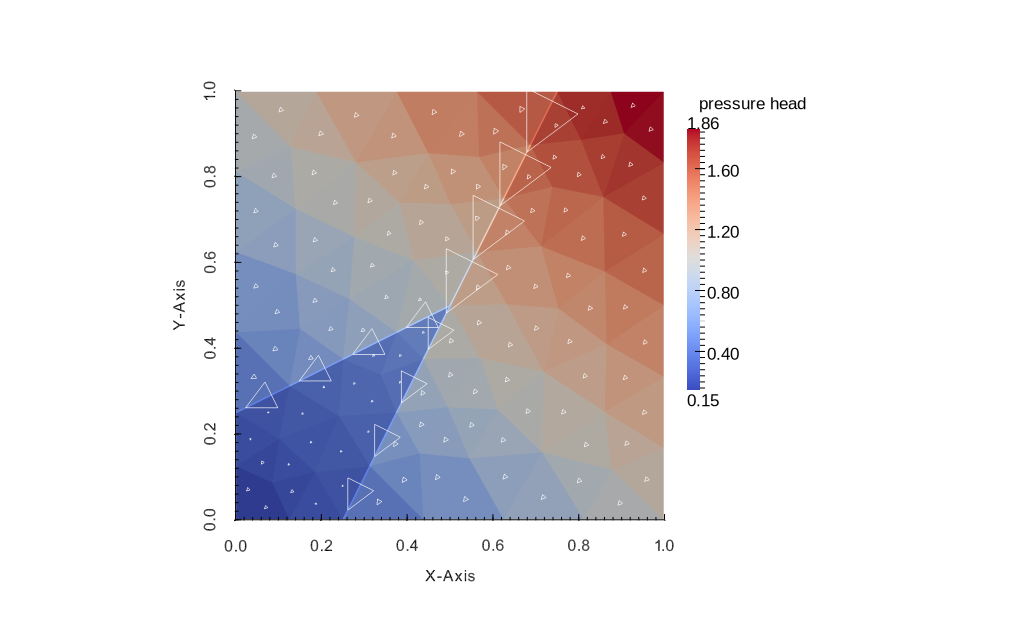
\includegraphics[scale=0.4]{./03_flow.pdf}
        % 03_flow.pdf: 508x402 pixel, 72dpi, 17.92x14.18 cm, bb=0 0 508 402
        \caption{Elementwise pressure head\\and velocity field (triangles).}
        \label{fig:tut-flow}
    \end{subfigure}
    ~
    \begin{subfigure}[b]{0.45\textwidth}
        \centering
        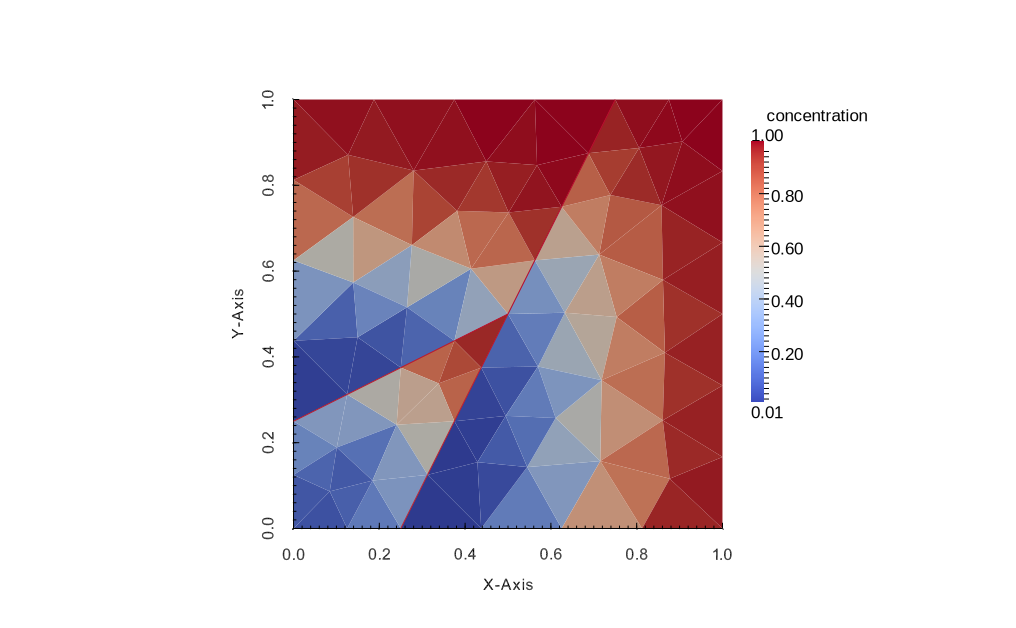
\includegraphics[scale=0.4]{./03_trans.pdf}
        % 03_trans.pdf: 509x402 pixel, 72dpi, 17.96x14.18 cm, bb=0 0 509 402
        \caption{Propagation of U235 from the inflow part of the boundary.}
        \label{fig:tut-trans}
    \end{subfigure}
    \caption{Results of the tutorial problem.}
    \label{fig:tutorial}
\end{figure}



The output files can be either \verb'*.msh' files accepted by the GMSH or one can use VTK format that can be post-processed by Paraview.

In the following chapter, we briefly describe structure of individual input files in particular the main INI file. In the last chapter, we describe
mathematical models and numerical methods used in the Flow123d.


\chapter{Mathematical models \\of physical reality}

Flow123d provides models for Dary flow in porous media as well as for the transport and reactions of soluted substances. In this section, we describe 
mathematical formulations of these models together with physical meaning and units of all involved quantities. Common and unique feature of all models is support of
domains with mixed dimension. Let $\Omega_{3} \subset \Real^3$ be an open set representing continuum approximation of porous and fractured medium.
Similarly, we consider open set $\Omega_2\subset \Real^2$ representing 2D fractures and open set $\Omega_1\subset \Real^3$ of 1D channels or preferential paths 
(see Fig \ref{fig:multi-dim}).
We assume that $\Omega_2$ and $\Omega_1$ are polygonal. For every dimension $d=1,2,3$, we introduce a triangulation $\mathcal{T}_{d}$ of the open set $\Omega_d$
that consists of finite elements $T_{d}^{i},$\ $i = 1,\dots,N_{E}^{d}$. The elements are simplexes that is tetrahedrons, triangles and lines.

\begin{figure}[h]
\centering
\includegraphics[width=10cm]{ground_fractures}
\caption{
    \label{fig:multi-dim}
    Scheme of a problem with domains of multiple dimensions.
}
\end{figure}

Present numerical methods requires meshes satisfying the compatibility conditions
\begin{equation}
        T_{d-1}^i \cap T_d \subset \mathcal{F}_d,   \qquad \text{where } \mathcal{F}_d = \bigcup_{k} \partial T_{d}^{k}
\end{equation}
and
\begin{equation}
        T_{d-1}^i \cap \mathcal{F}_d    \text{ is either $T_{d-1}^i$ or $\emptyset$}    
\end{equation}
for every $i\in\{1,\dots, N_{E}^{d-1}\}$, $j\in\{1,\dots,N_{E}^{d}\}$,  and $d=2,3$. That is the $(d-1)$-dimensional elements are either between $d$-dimensional elements and
match their sides or they poke out of $\Omega_d$. 

\input{darcy_flow}

\input{transport_model}


%% Copyright (C) 2007 Technical University of Liberec.  All rights reserved.
%
% Please make a following refer to Flow123d on your project site if you use the program for any purpose,
% especially for academic research:
% Flow123d, Research Centre: Advanced Remedial Technologies, Technical University of Liberec, Czech Republic
%
% This program is free software; you can redistribute it and/or modify it under the terms
% of the GNU General Public License version 3 as published by the Free Software Foundation.
%
% This program is distributed in the hope that it will be useful, but WITHOUT ANY WARRANTY;
% without even the implied warranty of MERCHANTABILITY or FITNESS FOR A PARTICULAR PURPOSE.
% See the GNU General Public License for more details.
%
% You should have received a copy of the GNU General Public License along with this program; if not,
% write to the Free Software Foundation, Inc., 59 Temple Place - Suite 330, Boston, MA 021110-1307, USA.

\normalsize
 \section*{Advection-Diffusion equation}
 
Solute transport is governed by advection equation which can be written in the form
\begin{equation}
 \frac{\partial c}{\partial t} + \boldsymbol{v} \frac{\partial c}{\partial x}  = 0, \label{Aeq}
\end{equation}
where $c$ is concentration $[M^3 \cdot L^{-3}]$, $t$ is time $[T]$, $v$ is velocity $[L \cdot T^{-1}]$, and $x$ is coordinate in cartesian system $[L]$.
Assuming solution which is constant on every element (cell centered finite volume method) and integrating equation (\ref{Aeq}) we get
    \begin{equation}
    \int\limits_{e_i} \frac{\partial c}{\partial t} dV + \int\limits_{e_i} \boldsymbol{v} \frac{\partial c}{\partial x} \, dV = 0. \notag 
    \end{equation}
    After some rearrangements we obtain on $i$-th element ($e_i$)
    \begin{equation}
    \frac{\partial c_i}{\partial t}  V_{i} + c \int\limits_{\partial e_i }  \boldsymbol{v} \, \mathbf{dS} = 0, \label{Aeqint} 
    \end{equation}
  where $c_i$ is average concentration in $e_i$ and $V_{i}$ its volume, $c$ will be specified later (there are two main possibilities - $c_i$ or concentration from neighbouring element).
    Term $\frac{\partial c}{\partial t}$ we approximate by explicit Euler difference
    \begin{equation}
     \frac{\partial c}{\partial \textrm{t}} \approx \frac{c_{i}^{n+1} - c_{i}^n}{\Delta t}. \label{expliciteuler}
    \end{equation}
    Where $\Delta t$ is a time step and upper index at $c_i$ means values in the discrete time steps $n+1$ and $n$.
    We assume that all elements have piecewise smooth element boudary $\partial e$ with outwards directed normal. Inside the area $\Omega$ we introduce internal flows.
    With respect to $e_i$, we define internal flow intake $U_{ij}^{-}$ (from element $e_j$) and
    internal flow drain $U_{ij}^{+}$ (to element $e_j$) as follows
    \begin{eqnarray}     
      U_{ij}^{-} = \text{min}(\int\limits_{\partial e_i \cap \partial e_j, i \ne j} \boldsymbol{v} \, \mathbf{dS},0), \notag \\
      U_{ij}^{+} = \text{max}(\int\limits_{\partial e_i \cap \partial e_j, i \ne j} \boldsymbol{v} \, \mathbf{dS},0). \label{iflux}  
    \end{eqnarray}
  Those flows realizes solute transport in the area $\Omega$. On the $\partial\Omega$ we define external flows which will be important for transport Dirichlet boundary  
  conditions. In the same way as for internal flows we assume
  (with respect to element $e_i$) external flow intake $U_{ij}^{e-}$ (from $\partial\Omega$) and external flow drain $U_{ij}^{e+}$ (to $\partial\Omega$).
    \begin{eqnarray}     
      U_{ik}^{e-} = \text{min}(\int\limits_{\partial e_i \cap \partial \Omega } \boldsymbol{v} \, \mathbf{dS},0), \notag \\
      U_{ik}^{e+} = \text{max}(\int\limits_{\partial e_i \cap \partial \Omega } \boldsymbol{v} \, \mathbf{dS},0). \label{eflux}  
    \end{eqnarray}
    Direction of the velocity $\boldsymbol{v}$, which affects sign of the $U$-terms is significant for the construction solution. For the solution
    stability it is suitable to use an upwind scheme, which can by written for finite difference on simple 1D geometry in the form
    \begin{eqnarray} 
      v>0 : \frac{\partial c}{\partial \textrm{x}} \approx \frac{c_{i}^n - c_{i-1}^n}{\Delta x},   \notag \\
      v<0 : \frac{\partial c}{\partial \textrm{x}} \approx \frac{c_{i+1}^n - c_i^n}{\Delta x}.   \label{upwind} 
    \end{eqnarray}
    This scheme can be interpreted as well as in finite volume method - in convection term one can get $c$ value opposite the flow of the quantity $\boldsymbol{v}$ direction.
      For every $e_i$ we introduce itemsets $\mathcal{N}_{i}, \mathcal{B}_{i}$ which contains indexes of neighbourging elements, local boundary conditions respectivelly.  
     Assuming upwind scheme, using (\ref{iflux}), (\ref{eflux}), and  (\ref{expliciteuler}) we can write solution of the equation (\ref{Aeqint}) 
    (relation between two consecutive time steps) on $e_i$ in the form 
    \begin{equation}
      c_i^{n+1} = c_i^n - \frac{\Delta t}{V_{i}} \left[ \sum_{j \in \mathcal{N}_{i}} \left[ U_{ij}^{+} c_i +  U_{ij}^{-} c_{j} \right] +
      \sum_{k \in \mathcal{B}_{i}}  \left[  U_{ik}^{e+} c_i +  U_{ik}^{e-} c_{B_{ik}} \right] \right]. \label{Aeqsol}
    \end{equation}
    Where $c_{B_{ik}}$ are values of Dirichlet boundary conditions which belong to $e_i$. Formula (\ref{Aeqsol}) can be rewritten into the matrix notation
    \begin{equation}
     \mathbf{c}^{n+1} = (\mathbf{I} + \Delta t \mathbf{A}) \cdot \mathbf{c}^{n} + \Delta t \mathbf{B} \cdot \mathbf{c_{B}}^{n} \label{AeqsolM}
    \end{equation}
  Where $\mathbf{c}$ is vector of $c_i^{n+1}$, $\mathbf{A}$ is a square matrix composed from $\frac{U_{ij}^{+}}{V_i}$, $\frac{U_{ij}^{-}}{V_i}$, and
  $\frac{U_{ij}^{e+}}{V_i}$. $\mathbf{B}$ is in general rectangular matrix composed from $\frac{U_{ij}^{e-}}{V_i}$ and $\mathbf{c_{B}}^{n}$ is  vector of Dirichlet
  boundary conditions.matrix definition. There is one stability condition for time step which is called Courant-Friedrich-Levy condition. 
  For the problem without sources/sinks it can be written as
  \begin{equation}
  \Delta t_{max} = \min_i \left( \frac{V_i}{ \sum\limits_{j}  U_{ij}^{+} + \sum\limits_{k}  U_{ik}^{e+} } \right) =
  \min_i \left( \frac{V_i}{ \sum\limits_{j} | U_{ij}^{-} | + \sum\limits_{k} | U_{ik}^{e-} | } \right). \label{cfl} 
  \end{equation}
  This condition has a physical interpretation, which can be understood as conservation law - volume that intakes/drains to/from element $e_i$ 
can not be higher then element volume $V_i$. From algebraical point of view this condition can be seen as a condition which bounds norm of the evolution operator as follows 
  \begin{equation}
  \| \mathbf{I} + \Delta t \mathbf{A} \quad \Delta t \mathbf{B} \| \le 1.
  \end{equation}
 \section*{Generalization}
  This approach can be used as well as for more general element connections -- for compatible/non-compatible element interconnection, if we know the flow integral
  values ($U_{ij}^{+}$ or $U_{ij}^{-}$). %Situation for more general case is in the picture (\ref{compmodel}).
      \begin{figure}[h]
        \begin{center}
        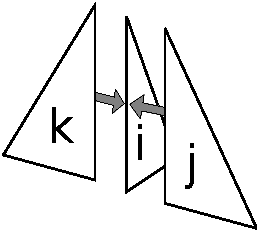
\includegraphics[scale=0.7]{obr7.pdf} 
	\caption{Edge with 3 elements}
	\label{edgemodel}
        \end{center}
      \end{figure}  
  The most general case of connection is relation among $n$ elements like in figure (\ref{edgemodel}). For this case we define
edge element indexset $\mathcal{G}_{l}$ that contains all the indexes of elements which sides make $l$-th edge ($g_l$), so that $\mathcal{G}_{l} = \{i,j,k\}$.
For $\mathcal{G}_{l}$ we introduce its subsets $\mathcal{G}_{ij}$, $\mathcal{G}_{ji}$, $\mathcal{G}_{ik}$, $\mathcal{G}_{ki}$, $\mathcal{G}_{kj}$, and $\mathcal{G}_{jk}$,
  where $\mathcal{G}_{ij} = \mathcal{G}_{ik} =  \mathcal{G}_{l} \backslash {i} = \{j,k\}$, $ \mathcal{G}_{ji} = \mathcal{G}_{jk} = \mathcal{G}_{l} \backslash {j} =\{i,k\}$, and
 $\mathcal{G}_{ki} = \mathcal{G}_{kj} = \mathcal{G}_{l} \backslash {k} =\{i,j\}$. It can be written in the same way for any edge $g$ with more than 3 elements, 
it is hold  $|\mathcal{G}_{g}| - 1 = |\mathcal{G}_{ab}|; \forall a,b \in \mathcal{G}_{g}$.
For $l$-th edge ($g_l$) we can define total edge flow $U_{g_{l}}$ eg. as
  \begin{eqnarray}
   U_{g_{l}} &=& \sum\limits_{m \in \mathcal{G}_{ji}}   \left[ U_{mj}^{+}   + \frac{ U_{jm}^{+}}{|\mathcal{G}_{ji}|} \right] = \sum\limits_{m \in \mathcal{G}_{jk}}  \left[ U_{mj}^{+}   +  \frac{ U_{jm}^{+}}{|\mathcal{G}_{jk}|} \right] \notag \\
	      &=& \sum\limits_{m \in \mathcal{G}_{ij}}  \left[ U_{mi}^{+}   +  \frac{ U_{im}^{+}}{|\mathcal{G}_{ij}|} \right] = \sum\limits_{m \in \mathcal{G}_{ik}} \left[  U_{mi}^{+} +  \frac{ U_{im}^{+}}{|\mathcal{G}_{ik}|} \right] \notag \\ 
	      &=& \sum\limits_{m \in \mathcal{G}_{ki}}  \left[ U_{mk}^{+}   +  \frac{ U_{km}^{+}}{|\mathcal{G}_{ki}|} \right] = \sum\limits_{m \in \mathcal{G}_{kj}}  \left[ U_{mk}^{+}   +  \frac{ U_{km}^{+}}{|\mathcal{G}_{kj}|} \right], \label{edgeflow}
  \end{eqnarray}
$U_{g_{l}}$ with respect to any $e_m$; $m \in \mathcal{G}_{l}$ has to have the same value because continuity equation, for assumed incompresible flow, has to
 be fulfilled in every edge. Edges with more than two elements and two and more nonzero intakes to edge realize an ideal mixing (to an average concentration) 
with weights which will be specified later. This fact modifies equation (\ref{Aeqsol}) on the general mesh into the form
    \begin{equation}
      c_i^{n+1} = c_i^n - \frac{\Delta t}{V_{i}} \left[ \sum_{j \in \mathcal{N}_{i}} \left[ U_{ij}^{+} c_i +  \frac{U_{ij}^{-}}{ \sum\limits_{k \in \mathcal{G}_{ij}}
      \left[ U_{ki}^{+} + \frac{U_{ik}^{+}}{|\mathcal{G}_{ij}|} \right] } \sum\limits_{k \in \mathcal{G}_{ij}} U_{ki}^{+} c_{k} \right] + 
      \sum_{k \in \mathcal{B}_{i}}  \left[  U_{ik}^{e+} c_i +  U_{ik}^{e-} c_{B_{ik}} \right] \right]. \label{Aeqsol2}
    \end{equation}
The edges with total edge flow $U_{g_{l}} = 0$ can occur breakdown in the equation (\ref{Aeqsol2}) via term $\sum\limits_{k \in \mathcal{G}_{ij}}\left[ U_{ki}^{+} + \frac{U_{ik}^{+}}{|\mathcal{G}_{ij}|} \right] = 0$.
This fact implies as well as numerator $U_{ij}^{-} = 0$. In order to avoid dividing by zero we have to assume computation only for nonzero flows.
Concentrations $c_k$, $k \in \mathcal{G}_{ij}$ that may intakes into element $e_i$ are weighted with weights 
\begin{equation}
 \alpha_k = \frac{U_{ki}^{+}}{\sum\limits_{k \in \mathcal{G}_{ij}} \left[ U_{ki}^{+} + \frac{U_{ik}^{+}}{|\mathcal{G}_{ij}|} \right] }, \label{weights}
\end{equation}
so that the ideal mixing in this edge leads to the average concentration 
\begin{equation}
 c_{av} = \frac{\sum\limits_{k \in \mathcal{G}_{ij}} U_{ki}^{+} c_{k}}{\sum\limits_{k \in \mathcal{G}_{ij}} \left[ U_{ki}^{+} + \frac{U_{ik}^{+}}{|\mathcal{G}_{ij}|} \right] }. \label{cav}
\end{equation}
Matrix notation is the same as in (\ref{AeqsolM}). Finally ...
%\chapter{Numerical methods}


%\input{decay}
%\input{semchem}


\chapter{File formats}
%\section{Input format}


\section{Main input file (CON file format)}
\label{sec:CONformat}

\begin{figure}
 \begin{center}
 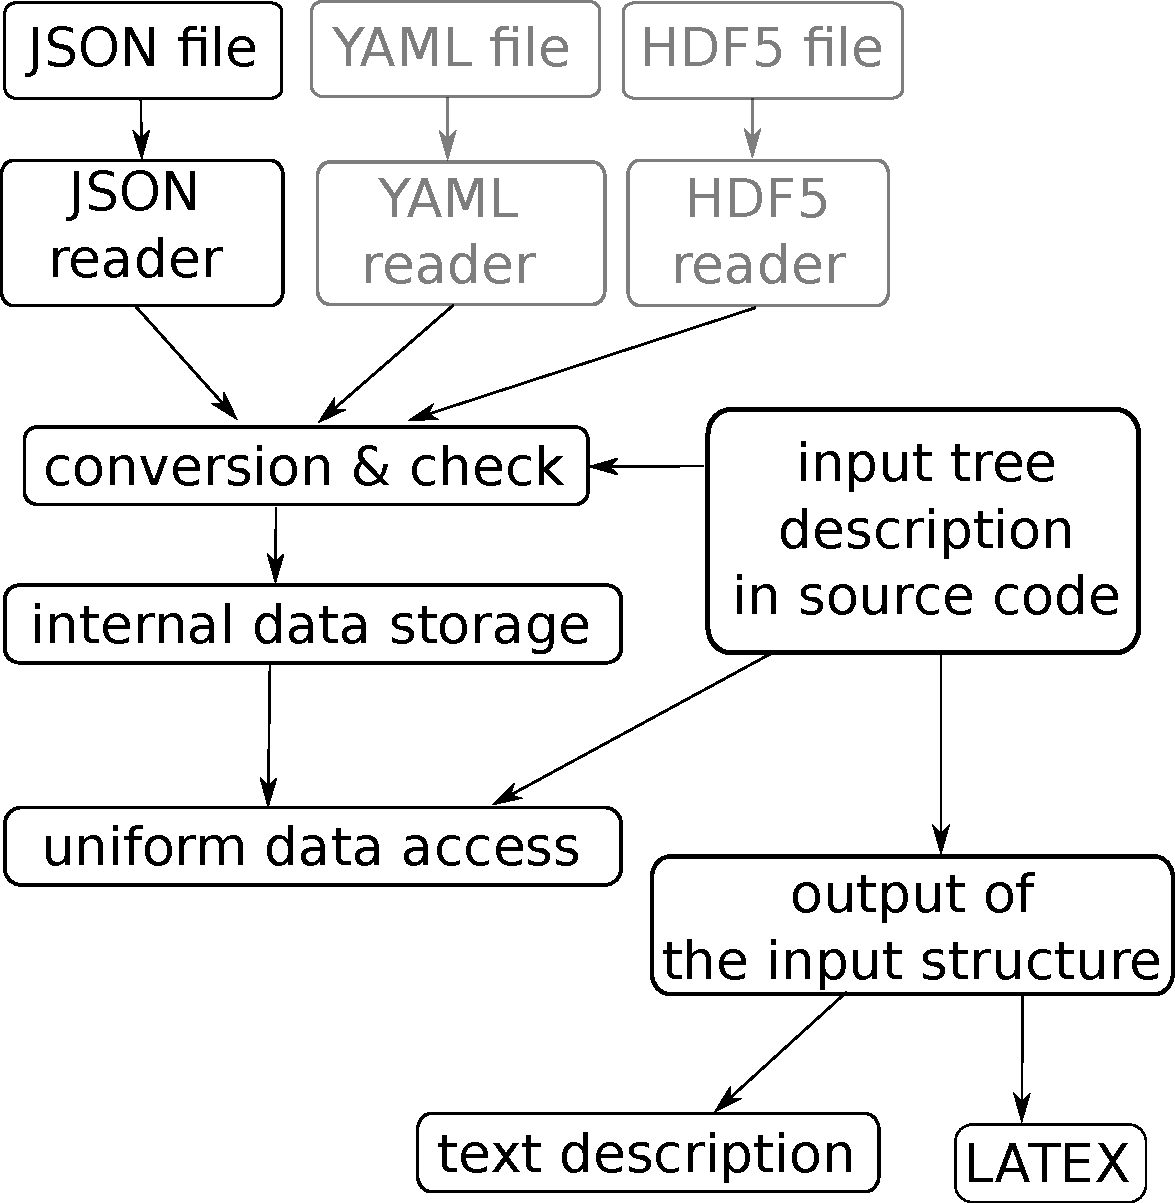
\includegraphics[scale=0.4]{./input_subsystem.pdf}
 % input_subsystem.pdf: 0x0 pixel, -2147483648dpi, 0.00x0.00 cm, bb=
 \caption{Sturucture of the input subsystem. Grey boxes are not implemented yet.}
 \label{fig:input_subsystem}
 \end{center}
\end{figure}

In this section, we shall describe structure of the main input file that is given through the parameter \verb'-s' on the command line.
The file formats of other files that are referenced from the main input file and used for input of the mesh or large field data
(e.g. the GMSH file format) are described in following sections. The input subsystem was designed with the aim to provide uniform initialization of 
C++ classes and data structures. Its structure is depicted on Figure \ref{fig:input_subsystem}.
The structure of the input is described by the Input Types Tree (ITT) of (usually static) objects which follows the structure of the classes.
The data from an input file are read by apropriate reader, their structure is checked against ITT and they are pushed into the Internal Storage Buffer (ISB).
An accessor object to the root data record is the result of the file reading. The data can be retrieved through accessors which combine 
raw data stored in in IBS with their meaning described in ITT. ITT can be printed out in various formats providing description of the input structure both for 
humans and other software.

Currently, the JSON input file format is only implemented and in fact it is slight extension of the JSON file format. On the other hand
the data for initialization of the C++ data structures are coded in particular way. Combination of this extension and restriction of the JSON file format produce 
what we call CON (C++ object notation) file format.


\subsection{JSON for humans}

Basic syntax of the CON file is very close to the JSON file format with only few extensions, namely:
\begin{itemize}
\item You can use C++ (or JavaScript) comments. One line comments \verb'//' and multi-line comments \verb'/* */'.
\item The quoting of the keys is optional if they do not contain spaces (holds for all CON keys).
\item You can use equality sign \verb'=' instead of colon \verb':' for separation of keys and values in JSON objects.
\item You can use any whitespace to separate tokens in JSON object or JSON array.
\end{itemize}
The aim of these extensions is to simplify writing input files manually. However these extensions can be easily filtered out and converted to 
the generic JSON format. For the description of the JSON format we refer to \url{http://www.json.org/}. 

\subsection{CON constructs}
The CON file format constructs are designed for initialization of C++ strongly typed variables. The primitive data types can be initialized from 
the primitive CON constructs: 
\begin{itemize}
 \item {\it Bool} --- initialized from the JSON keywords \verb'true' and \verb'false'.
 \item {\it Double}, {\it Integer} --- initialized from JSON numeric data. 
 \item {\it String}, {\it FileName}, {\it Selections} --- initialized from JSON strings
\end{itemize}
Selections are typed like the C++ enum types that are initialized from them.
Various kind of containers can be initialized by the {\it Array} construct, that is an JSON array with elements of the same CON type. 
The C++ structures and classes can be initialize from the {\it Record} construct, which is represented by a JSON object. However, in constrast to JSON,
these Records have different types in similar way as the strong typed C++ structures. The types are described by ITT of the particular program
which can be printed out in several formats, in particular description of ITT for Flow123d forms content of Chapter \ref{chapter:input-tree-reference}.
In order to allow certain kind of polymorphism, we introduce also the {\it AbstractRecord} construct, where the type of the record is not given by ITT but 
can be chosen as part of the input. 

\subsection{CON special keys}
All keys in Records should be in lower case, possibly using digits and underscore. The keys all in upper case are reserved for special function in the 
CON file. These are:
\begin{description}

\item[TYPE key]:
\begin{verbatim}
TYPE=<Selection of AbstractRecord>
\end{verbatim}
Is used to specify particular type of an AbstractRecord. This way you can choose which particular implementation of an abstract C++ class should be instantiated.
The value of the key is a string from the Selection that consists of names of Records that was declared as descendants of the AbstractRecord.


%\item[INCLUDE\_RECORD]:\\
%This is a simple inclusion of another file as a content of a record:
%\begin{verbatim}
%{
%        INCLUDE_RECORD = "<file name>"
%}
%\end{verbatim}
%
%\item[INCLUDE\_ARRAY]:\\
%\begin{verbatim}
%array=
%{
%        INCLUDE_ARRAY = "<file name>"
%        FORMAT = "<format string>"
%}       
%\end{verbatim}
%The reader will substitute the include record by a sequentially accessible array. The file has fixed number of 
%space separated data fields on every line. Every line becomes one element in the array of type record. Every line forms a 
%record with key names given by the \verb'<format string>' 
%and corresponding data taken form the line.

%The key difference compared to regular JSON arrays is that included arrays can be accessed only sequentially 
%within the program and thus we minimize reader memory overhead for large input data. The idea is to translate raw data into structured
%format and use uniform access to the data.

%Basic syntax for format string could be an array of strings --- formats of individual columns.
%Every format string is an address of key that is given the column. Onother possibility is to give an arbitrary 
%JSON file, where all values are numbers of columns where to take the value.

%[\dots better specify format string]


%Possible extensions:
% have sections in the file for setting time dependent data
% have number of lines at the beginning
% have variable format
% allow vectors in the 'line records']

\item[REF key]:
\begin{verbatim}
{ REF=<address> }
\end{verbatim}
The record in input file that contains only the key \verb'REF' is replaced by the JSON entity that is referenced by the \verb'<address>'. 
The address is a string with format similar to UNIX path, i.e. with grammar
\begin{verbatim}
    <address> = <address> / <item>
              = <item>  
              = <null>
    <item> = <index>
           = <key>
           = ..
\end{verbatim}
where \verb'index' is non-negative integer and key is valid CON record key (lowercase, digits, underscores).
The address can be absolute or relative identification of an entity. The relative address is relative to the entity in which the reference record is contained.
One can use two dots \verb'".."' to move to parent entity.

Example:
\begin{verbatim}
mesh={
        file_name="xyz"
}
array=[
        {x=1 y=0}       
        {x=2 y=0}
        {x=3 y=0}
]               
outer_record={
        output_file="x_out"
        inner_record={
                output_file={REF="../output_file"} // value "x_out"
        }
        x={REF="/array/2/x"}                       // value "3"
        f_name={REF="/mesh/file_name"}             // value "xyz"
}       
\end{verbatim}
\end{description}

\subsection{Record types}
A Record type is given by the set of key specifications, which in turn consist from: key name, type of value and default value specification.
Default value specification can be:
\begin{description} 
 \item[obligatory] --- means no default value, which has to be specified at input. 
 \item[optional] --- means no default value, but value is needs not to be specified. Unspecified value usually means that you turn off some functionality.
 \item[default at declaration] --- the default value is explicitly given in declaration and is automatically provided by the input subsystem if needed
 \item[default at read time] --- the default value is provided at read time, usually from some other variable. In the documentation, 
 there is only textual description where the default value comes from.
\end{description}

\subsubsection{Implicit creation of composed entities}
Consider a Record type in which all keys have default values (possibly except one). Then the specification
of the Record can contain a {\it key for default construction}. User can specify only the value of this particular key instead of the whole record, all other keys are initialized from its default values.
Moreover, an AbstractRecord type may have a default value for the \verb'TYPE' key.
This allows to express simple tasks by simple inputs but still make complex inputs possible. 
Similar functionality holds for arrays. If the user sets a non-array value where an array is expected the reader provides an array with a unique element holding the given value.


\section{Important Record types of Flow123d input}


\subsection{Mesh record}
\label{sec:Mesh}
The \hyperlink{IT::Mesh}{mesh record} provides initialization for the computational mesh consisting of points, lines, triangles and tetrahedrons in 3D space.
Currently, we support only GMSH mesh file format \href{http://geuz.org/gmsh/doc/texinfo/gmsh.html#MSH-ASCII-file-format}{MSH ASCII}. 
The input file is provided by the key \hyperA{Mesh::mesh-file}{{\tt mesh\_file}}. The file format allows to group elements into {\it regions} identified either by ID number or by string label. 
The regions with labels starting with the dot character are treated as {\it boundary regions}. Their elements are removed from the computational domain, however they can be used to specify boundary
conditions. Other regions are called {\it bulk regions}. User can create new labeled regions through the key 
\hyperA{Mesh::regions}{{\tt regions}}, the new region can be specified either by its ID
or by list of IDs of its elements. The latter possibility overrides original region assigned to the elements, which can be useful for specification of small areas ``ad hoc''.
The key \hyperA{Mesh::sets}{{\tt sets}} allows specification of sets of regions in terms of list of region IDs or labels and basic set operations. The difference between regions and sets is that
regions form disjoint covering of elements, the sets, however, may overlap. There are three predefined region sets: ``ALL'', ``BOUNDARY'', ``BULK''.


\subsection{Field records}
\label{}
A general time and space dependent, scalar, vector, or  tensor valued function can be specified through the family of abstract records 
Field $R^m -> \mathcal{S}$, where $m$ is currently always $m=3$ and $\mathcal{S}$ is a specification of the target space, which can be:
\begin{itemize}
 \item {\bf $\mathcal{T}$} --- scalar valued field, with scalars of type $\mathcal{T}$
 \item {\bf $\mathcal{T}[d]$} --- vector valued field, with vector of fixed size $d$ and elements of type $\mathcal{T}$
 \item {\bf $\mathcal{T}[\tt n]$} --- vector valued field, with vector of variable size (given by some input) and elements of type $\mathcal{T}$
 \item {\bf $\mathcal{T}[d, d]$} --- tensor valued field, with square tensor of fixed size and elements of type $\mathcal{T}$
\end{itemize}
the scalar types can be
\begin{itemize}
 \item {\bf Real} --- scalar real valued field
 \item {\bf Int}  --- scalar integer valued field
 \item {\bf Enum} --- scalar non negative integer valued field, should be convertible to appropriate C++ enum type
\end{itemize}

Each of these abstract record has the same set of descendants which implement various algorithms to specify and compute values of the field. These are
\begin{description}
 \item[FieldConstant] --- field that is constant in space
 \item[FieldFormula] --- field that is given by runtime parsed formula using $x,y,z,t$ coordinates. The \href{http://warp.povusers.org/FunctionParser/}{Function Parser} library is used
 with syntax rules described \href{http://warp.povusers.org/FunctionParser/fparser.html#literals}{here}.
 \item[FieldPython] --- field can be implemented by Python script either specified by string (key \hyperA{FieldPython::script-string}{{\tt script\_string}}) 
 or in external file (key \hyperA{FieldPython::script-file}{{\tt script\_file}}. 
 \item[FieldElementwise] --- discrete field, currently only piecewise constant field on elements is supported, the field can given by 
 the \href{http://geuz.org/gmsh/doc/texinfo/gmsh.html#MSH-ASCII-file-format}{MSH ASCII} file specified in key \hyperA{FieldElementwise::gmsh-file}{{\tt gmsh\_file}} and field name in the file given 
 by key \hyperA{FieldElementwise::field-name}{{\tt field\_name}}. The file must contain same mesh as is used for computation.
 \item[FieldInterpolated] --- allows interpolation between different meshes. Not yet fully supported.
\end{description}

Several automatic conversions are implemented. Scalar values can be used to set constant vectors or tensors. Vector value of size $d$ can be used to set diagonal tensor $d\times d$.
Vector value of size $d(d-1)/2$, e.g. $6$ for $d=3$, can be used to set symmetric tensor. These rules apply only for FieldConstant and FieldFormula.
Moreover, all Field abstract types have default value \verb'TYPE=FieldConstant'. Thus you can just use the constant value instead of the whole record.

Examples:
\begin{verbatim}
constant_scalar_function = 1.0
// is same as
constant_scalar_function = {
  TYPE=FieldConstant,
  value=1.0
}

conductivity_tensor = [1 ,2, 3]
// is same as
conductivity_tensor = {
    TYPE=FieldConstant,
    value=[[1,0,0],[0,2,0],[0,0,3]]
}

concentration = {
    TYPE=FieldFormula,
    value="x+y+z"
}
//is same as (provided the vector has 2 elements)
concentration = {
    TYPE=FieldFormula,
    value=["x+y+z", "x+y+z"]
}       
\end{verbatim}

\subsection{Field data for equations}
Every equation record has keys \verb'bulk\_data' and \verb'bc_data'. Both have the same structure, however, the first one is intended to set the bulk fields (on bulk regions)
while the second serves for initialization of the boundary fields (on boundary regions). These keys contains an array of region-time initialization records
like the \hyperlink{IT::DarcyFlowMH-Steady-BulkData}{BulkData} record of the DarcyFlow equation. Every such record specify fields on particular region 
(keys \hyperA{DarcyFlowMH-Steady-BulkData::region}{{\tt region}} and \hyperA{DarcyFlowMH-Steady-BulkData::rid}{{\tt rid}} ) or on a region set 
(key \hyperA{DarcyFlowMH-Steady-BulkData::r-set}{{\tt r\_set}}) starting from the time specified by the key \hyperA{DarcyFlowMH-Steady-BulkData::time}{{\tt time}}.
The array is processed sequentially and latter values overwrites the previous ones. Times should form a non-decreasing sequence.

Example:
\begin{verbatim}
bulk_data = [   
    { // time=0.0  - default value
        r_set="BULK"
        conductivity=1   // setting the conductivity field on all regions
    }
    {
        region="2d_part"
        conductivity=2  // overwriting the previous value
    }
    {   time=1.0
        region="2d_part"
        conductivity={
            // from time=1.0 we switch to the linear function in time
            TYPE=FieldFormula
            value="2+t"      
        }    
    }
    {   time=2.0
        region="2d_part"
        conductivity={
            // from time=2.0 we switch to elementwise field, but only
            // on the region "2d_part"
            TYPE=FieldElementwise
            gmsh_file="./input/data.msh"
            field_name="conductivity"
        }
    }    
]               
\end{verbatim}



% Copyright (C) 2007 Technical University of Liberec.  All rights reserved.
%
% Please make a following refer to Flow123d on your project site if you use the program for any purpose,
% especially for academic research:
% Flow123d, Research Centre: Advanced Remedial Technologies, Technical University of Liberec, Czech Republic
%
% This program is free software; you can redistribute it and/or modify it under the terms
% of the GNU General Public License version 3 as published by the Free Software Foundation.
%
% This program is distributed in the hope that it will be useful, but WITHOUT ANY WARRANTY;
% without even the implied warranty of MERCHANTABILITY or FITNESS FOR A PARTICULAR PURPOSE.
% See the GNU General Public License for more details.
%
% You should have received a copy of the GNU General Public License along with this program; if not,
% write to the Free Software Foundation, Inc., 59 Temple Place - Suite 330, Boston, MA 021110-1307, USA.


\section{Mesh and data file format MSH ASCII}
\label{mesh_file}

Currently, the only supported format for the computational mesh is MSH ASCII format used
by the GMSH software. You can find its documentation on:

\url{http://geuz.org/gmsh/doc/texinfo/gmsh.html#MSH-ASCII-file-format}

The scheme of the file is as follows:
\begin{verbatim}
$MeshFormat
<format version>
$EndMeshFormat

$PhysicalNames
<number of items>
<dimension>     <region ID>     <region label>
...
$EndPhysicalNames

$Nodes
<number of nodes>
<node ID> <X coord> <Y coord> <Z coord>
...
$EndNodes

$Elements
<number of elements>
<element ID> <element shape> <n of tags> <tags> <nodes>
...
$EndElements

$ElementData
<n of string tags>
    <field name>
    <interpolation scheme>
<n of double tags>
    <time>
<n of integer tags>
    <time step index>
    <n of components>
    <n of items>
    <partition index>
<element ID> <component 1> <component 2> ...
...
$EndElementData
\end{verbatim}
Detailed description of individual sections:
\begin{description}
 \item[{\tt PhysicalNames}] --- assign labels to region IDs
 \item[{\tt Nodes}] --- {\tt <number of nodes>} is also number of data lines that follows. 
    Node IDs are unique but need not to form an aritmetic sequance. Coordinates are float numbers.
 \item[{\tt Elements}] --- Element IDs are unique but need not to form an aritmetic sequence. 
    {\tt <element shape>} is integer code of the shape, we support only points (15), lines (1), triangles (2), and tetrahedrons (4).
    Default number of tags is 3. The first is the region ID, the second is ID of the geometrical entity (that was used in original geometry file from which the mesh was generated),
    and the third tag is the partition number. {\tt nodes} is list of node IDs with size according to the element shape.
 \item[{\tt ElementData}] --- the header has 2 string tags, 1 double tag, and 4 integer tags with default meaning. For the purpose of the \verb'FieldElementwise' the tags
    \verb'<field name>', \verb'<n of components>', and \verb'<n of items>' are obligatory.
\end{description}


%%%%%%%%%%%%%%%%%%%%%%%%%%%%%%%%%%%%%%%%%%%%%%%%%%%%%%%%%%%%%%%%%%%%%%%%%%%%%%%%%%%%%%%%%%%%%


% Copyright (C) 2007 Technical University of Liberec.  All rights reserved.
%
% Please make a following refer to Flow123d on your project site if you use the program for any purpose,
% especially for academic research:
% Flow123d, Research Centre: Advanced Remedial Technologies, Technical University of Liberec, Czech Republic
%
% This program is free software; you can redistribute it and/or modify it under the terms
% of the GNU General Public License version 3 as published by the Free Software Foundation.
%
% This program is distributed in the hope that it will be useful, but WITHOUT ANY WARRANTY;
% without even the implied warranty of MERCHANTABILITY or FITNESS FOR A PARTICULAR PURPOSE.
% See the GNU General Public License for more details.
%
% You should have received a copy of the GNU General Public License along with this program; if not,
% write to the Free Software Foundation, Inc., 59 Temple Place - Suite 330, Boston, MA 021110-1307, USA.
\parindent = 0pt

\section*{Output data}
\subsection{Output data fields of water flow modul}
\subsection{Output data fields of transport}

\subsection{GMSH viewer remarks}
\subsection{Paraview viewer remarks}
%\input{tso_10} 
%
\parindent = 0pt

\section*{ASCII post-processing file format version 1.2}
File format of this file comes from the GMSH system. 
Following text is copied from the GMSH documentation.\\[0.5em]

{\tt =============== BEGIN OF INSERTED TEXT ===============}\\[0.3em] 

The ASCII post-processing file is divided in several sections: one format
section, enclosed between {\tt \$PostFormat}-{\tt \$EndPostFormat} tags, and
one or more post-processing views, enclosed between
{\tt \$View}-{\tt \$EndView} tags:

\begin{fileformat}
\$PostFormat\\
1.2 \vari{file-type} \vari{data-size}\\
\$EndPostFormat\\
\$View\\
\vari{view-name} \vari{nb-time-steps}\\
\vari{nb-scalar-points} \vari{nb-vector-points} \vari{nb-tensor-points}\\
\vari{nb-scalar-lines} \vari{nb-vector-lines} \vari{nb-tensor-lines}\\
\vari{nb-scalar-triangles} \vari{nb-vector-triangles} \vari{nb-tensor-triangles}\\
\vari{nb-scalar-quadrangles} \vari{nb-vector-quadrangles} \vari{nb-tensor-quadrangles} \\
\vari{nb-scalar-tetrahedra} \vari{nb-vector-tetrahedra} \vari{nb-tensor-tetrahedra} \\
\vari{nb-scalar-hexahedra} \vari{nb-vector-hexahedra} \vari{nb-tensor-hexahedra}\\
\vari{nb-scalar-prisms} \vari{nb-vector-prisms} \vari{nb-tensor-prisms}\\
\vari{nb-scalar-pyramids} \vari{nb-vector-pyramids} \vari{nb-tensor-pyramids}\\
\vari{nb-text2d} \vari{nb-text2d-chars} \vari{nb-text3d} \vari{nb-text3d-chars}\\
$<$\vari{time-step-values}$>$\\
$<$\vari{scalar-point-values}$>$\\
$<$\vari{vector-point-values}$>$\\
$<$\vari{tensor-point-values}$>$\\
$<$\vari{scalar-line-values}$>$\\
$<$\vari{vector-line-values}$>$\\
$<$\vari{tensor-line-values}$>$\\
$<$\vari{scalar-triangle-values}$>$\\
$<$\vari{vector-triangle-values}$>$\\
$<$\vari{tensor-triangle-values}$>$\\
$<$\vari{scalar-quadrangle-values}$>$\\
$<$\vari{vector-quadrangle-values}$>$\\
$<$\vari{tensor-quadrangle-values}$>$\\
$<$\vari{scalar-tetrahedron-values}$>$\\
$<$\vari{vector-tetrahedron-values}$>$\\
$<$\vari{tensor-tetrahedron-values}$>$\\
$<$\vari{scalar-hexahedron-values}$>$\\
$<$\vari{vector-hexahedron-values}$>$\\
$<$\vari{tensor-hexahedron-values}$>$\\
$<$\vari{scalar-prism-values}$>$\\
$<$\vari{vector-prism-values}$>$\\
$<$\vari{tensor-prism-values}$>$\\
$<$\vari{scalar-pyramid-values}$>$\\
$<$\vari{vector-pyramid-values}$>$\\
$<$\vari{tensor-pyramid-values}$>$\\
$<$\vari{text2d}$>$ $<$\vari{text2d-chars}$>$\\
$<$\vari{text3d}$>$ $<$\vari{text3d-chars}$>$\\
\$EndView
\end{fileformat}

where:
\begin{description}
\item[\vari{file-type}]
is an integer equal to 0 in the ASCII file format.

\item[\vari{data-size}]
is an integer equal to the size of the floating point numbers used in the
file (usually, \vari{data-size} = sizeof(double)).

\item[\vari{view-name}]
is a string containing the name of the view (max. 256 characters).

\item[\vari{nb-time-steps}]
is an integer giving the number of time steps in the view.

\item[\vari{nb-scalar-points}, \vari{nb-vector-points}, \vari{\dots}]
are integers giving the number of scalar points, vector points,\dots
in the view.

\item[\vari{nb-text2d}, \vari{nb-text3d}]
are integers giving the number of 2D and 3D text strings in the
view. 

\item[\vari{nb-text2d-chars}, \vari{nb-text3d-chars}]
are integers giving the total number of characters in the 2D and 3D strings.

\item[\vari{time-step-values}]
is a list of \vari{nb-time-steps} double precision numbers giving the value
of the time (or any other variable) for which an evolution was saved.

\item[\vari{scalar-point-value}, \vari{vector-point-value}, \vari{\dots}]
are lists of double precision numbers giving the node coordinates and the
values associated with the nodes of the \vari{nb-scalar-points} scalar
points, \vari{nb-vector-points} vector points,\dots, for each of the
\vari{time-step-values}.

For example, \vari{vector-triangle-value} is defined as:
\begin{fileformat}
\vari{coord1-node1} \vari{coord1-node2} \vari{coord1-node3}\\
\vari{coord2-node1} \vari{coord2-node2} \vari{coord2-node3}\\
\vari{coord3-node1} \vari{coord3-node2} \vari{coord3-node3}\\
\vari{comp1-node1-time1} \vari{comp2-node1-time1} \vari{comp3-node1-time1}\\
\vari{comp1-node2-time1} \vari{comp2-node2-time1} \vari{comp3-node2-time1}\\
\vari{comp1-node3-time1} \vari{comp2-node3-time1} \vari{comp3-node3-time1}\\
\vari{comp1-node1-time2} \vari{comp2-node1-time2} \vari{comp3-node1-time2}\\
\vari{comp1-node2-time2} \vari{comp2-node2-time2} \vari{comp3-node2-time2}\\
\vari{comp1-node3-time2} \vari{comp2-node3-time2} \vari{comp3-node3-time2}\\
\dots
\end{fileformat}

\item[\vari{text2d}]
is a list of 4 double precision numbers:
\begin{fileformat}
\vari{coord1} \vari{coord2} \vari{style} \vari{index}
\end{fileformat}
where \vari{coord1} and \vari{coord2} give the coordinates of the leftmost
element of the 2D string in screen coordinates, \vari{index} gives the
starting index of the string in \vari{text2d-chars} and \vari{style} is
currently unused.

\item[\vari{text2d-chars}]
is a list of \vari{nb-text2d-chars} characters. Substrings are separated with
the `$^\wedge$' character (which is a forbidden character in regular strings).

\item[\vari{text3d}]
is a list of 5 double precision numbers
\begin{fileformat}
\vari{coord1} \vari{coord2} \vari{coord3} \vari{style} \vari{index}
\end{fileformat}
where \vari{coord1}, \vari{coord2} and \vari{coord3} give the coordinates of
the leftmost element of the 3D string in model (real world) coordinates,
\vari{index} gives the starting index of the string in \vari{text3d-chars} and
\vari{style} is currently unused.

\item[\vari{text3d-chars}]
is a list of \vari{nb-text3d-chars} chars. Substrings are separated with the
`$^\wedge$' character.
\end{description}
 
{\tt =============== END OF INSERTED TEXT ===============}\\[0.5em]

More information about GMSH can be found at its homepage:\\
\leftline{\tt http://www.geuz.org/gmsh/}\\

\subsection*{Comments concerning {\tt FFLOW20}:}
\begin{itemize}
  \item {\tt FFLOW20} generates {\tt .POS} file with four views: Elements'
     pressure, edges' pressure, interelement fluxes and complex view. First
     three views shows "raw data", results obtained by the solver without any
     interpolations, smoothing etc. The fourth view contains data processed in
     this way.
     \begin{description}
       \item[Elements' pressure:] Contains only \vari{scalar-triangle-values}.
         Triangles are the same as the elements of the original mesh. We
         prescribe constant value of the pressure on the element, as it was
         calculated by the solver as the unknown $p$. Therefore, the three
         values on every triangle are the same.
       \item[Edge pressure:]  Contains only \vari{scalar-line-values}. The
         lines are the same as the edges of the elements of the original
         mesh. We prescribe constant value of the pressure on the edge, as it
         was calculated by the solver as the unknown $\lambda$. Therefore, the
         two values on every edge are the same.
       \item[Interelement flux:] Contains \vari{vector-point-values} and
         \vari{scalar-triangle-values}. The \vari{scalar-triangle-values}
         carry no information, all values are set to 0, these are in the file
         only to define a shape of the elements. The points for the
         \vari{vector-point-values} are midpoints of the sides of the
         elements. The vectors are calculated as $u{\bf n}$, where $u$ is
         value of the flux calculated by the solver and ${\bf n}$ is
         normalized vector of outer normal of the element's side.
       \item[Complex view:] Contains \vari{scalar-triangle-values} and
         \vari{vector-point-values}. The \vari{scalar-triangle-values} shows the
         shape of the pressure field. The triangles are the the same as the
         elements of the original mesh. Values of pressure in nodes are
         interpolated from $p$s and $\lambda$s. The \vari{vector-point-values}
         shows the velocity of the flow in the centres of the elements.
     \end{description}
\end{itemize}

   


%\chapter{Test and tutorial problems}
%\input{tests}

\chapter{Main input file reference}
\label{chapter:input-tree-reference}
% support macros


% generated file

\begin{RecordType}{\HTRaised{IT::Root}{Root}}{}{}{\relax}{Root record of JSON input for Flow123d.}
\KeyItem{\hyperB{Root::problem}{problem}}{abstract type: \hyperlink{IT::Problem}{Problem}}{\textless\it obligatory\textgreater}{}{Simulation problem to be solved.}
\KeyItem{\hyperB{Root::pause-after-run}{pause\_after\_run}}{Bool}{false}{}{If true, the program will wait for key press before it terminates.}
\KeyItem{\hyperB{Root::output-streams}{output\_streams}}{Array  of record: \hyperlink{IT::OutputStream}{OutputStream}}{\textless\it optional\textgreater}{}{Array of formated output streams to open.}
\end{RecordType}

\begin{AbstractType}{\HTRaised{IT::Problem}{Problem}}{}{}{The root record of description of particular the problem to solve.}
\Descendant{\hyperlink{IT::SequentialCoupling}{SequentialCoupling}}
\end{AbstractType}

\begin{RecordType}{\HTRaised{IT::SequentialCoupling}{SequentialCoupling}}{\hyperlink{IT::Problem}{Problem}}{}{}{Record with data for a general sequential coupling.
}
\KeyItem{\hyperB{SequentialCoupling::TYPE}{TYPE}}{selection: Problem\_TYPE\_selection}{SequentialCoupling}{}{Sub-record selection.}
\KeyItem{\hyperB{SequentialCoupling::description}{description}}{String (generic)}{\textless\it optional\textgreater}{}{Short description of the solved problem.
Is displayed in the main log, and possibly in other text output files.}
\KeyItem{\hyperB{SequentialCoupling::mesh}{mesh}}{record: \hyperlink{IT::Mesh}{Mesh}}{\textless\it obligatory\textgreater}{}{Computational mesh common to all equations.}
\KeyItem{\hyperB{SequentialCoupling::time}{time}}{record: \hyperlink{IT::TimeGovernor}{TimeGovernor}}{\textless\it optional\textgreater}{}{Simulation time frame and time step.}
\KeyItem{\hyperB{SequentialCoupling::primary-equation}{primary\_equation}}{abstract type: \hyperlink{IT::DarcyFlowMH}{DarcyFlowMH}}{\textless\it obligatory\textgreater}{}{Primary equation, have all data given.}
\KeyItem{\hyperB{SequentialCoupling::secondary-equation}{secondary\_equation}}{abstract type: \hyperlink{IT::Transport}{Transport}}{\textless\it optional\textgreater}{}{The equation that depends (the velocity field) on the result of the primary equation.}
\end{RecordType}

\begin{RecordType}{\HTRaised{IT::Mesh}{Mesh}}{}{}{\hyperlink{}{}}{Record with mesh related data.}
\KeyItem{\hyperB{Mesh::mesh-file}{mesh\_file}}{input file name}{\textless\it obligatory\textgreater}{\hyperlink{}{}}{Input file with mesh description.}
\KeyItem{\hyperB{Mesh::regions}{regions}}{Array  of record: \hyperlink{IT::Region}{Region}}{\textless\it optional\textgreater}{}{List of additional region definitions not contained in the mesh.}
\KeyItem{\hyperB{Mesh::sets}{sets}}{Array  of record: \hyperlink{IT::RegionSet}{RegionSet}}{\textless\it optional\textgreater}{}{List of region set definitions. There are three region sets implicitly defined:
ALL (all regions of the mesh), BOUNDARY (all boundary regions), and BULK (all bulk regions)}
\end{RecordType}

\begin{RecordType}{\HTRaised{IT::Region}{Region}}{}{}{}{Definition of region of elements.}
\KeyItem{\hyperB{Region::name}{name}}{String (generic)}{\textless\it obligatory\textgreater}{}{Label (name) of the region. Has to be unique in one mesh.
}
\KeyItem{\hyperB{Region::id}{id}}{Integer [0, ]}{\textless\it obligatory\textgreater}{}{The ID of the region to which you assign label.}
\KeyItem{\hyperB{Region::element-list}{element\_list}}{Array  of Integer [0, ]}{\textless\it optional\textgreater}{}{Specification of the region by the list of elements. This is not recomended}
\end{RecordType}

\begin{RecordType}{\HTRaised{IT::RegionSet}{RegionSet}}{}{}{}{Definition of one region set.}
\KeyItem{\hyperB{RegionSet::name}{name}}{String (generic)}{\textless\it obligatory\textgreater}{}{Unique name of the region set.}
\KeyItem{\hyperB{RegionSet::region-ids}{region\_ids}}{Array  of Integer [0, ]}{\textless\it optional\textgreater}{}{List of region ID numbers that has to be added to the region set.}
\KeyItem{\hyperB{RegionSet::region-labels}{region\_labels}}{Array  of String (generic)}{\textless\it optional\textgreater}{}{List of labels of the regions that has to be added to the region set.}
\KeyItem{\hyperB{RegionSet::union}{union}}{Array [2, 2] of String (generic)}{\textless\it optional\textgreater}{}{Defines region set as a union of given pair of sets. Overrides previous keys.}
\KeyItem{\hyperB{RegionSet::intersection}{intersection}}{Array [2, 2] of String (generic)}{\textless\it optional\textgreater}{}{Defines region set as an intersection of given pair of sets. Overrides previous keys.}
\KeyItem{\hyperB{RegionSet::difference}{difference}}{Array [2, 2] of String (generic)}{\textless\it optional\textgreater}{}{Defines region set as a difference of given pair of sets. Overrides previous keys.}
\end{RecordType}

\begin{RecordType}{\HTRaised{IT::TimeGovernor}{TimeGovernor}}{}{}{}{Setting of the simulation time. (can be specific to one eqaution)}
\KeyItem{\hyperB{TimeGovernor::start-time}{start\_time}}{Double }{0.0}{}{Start time of the simulation.}
\KeyItem{\hyperB{TimeGovernor::end-time}{end\_time}}{Double }{\textless\it obligatory\textgreater}{}{End time of the simulation.}
\KeyItem{\hyperB{TimeGovernor::init-dt}{init\_dt}}{Double [0, ]}{\textless\it optional\textgreater}{}{Initial guess for the time step. The time step is fixed if hard time step limits are not set.}
\KeyItem{\hyperB{TimeGovernor::min-dt}{min\_dt}}{Double [0, ]}{"Machine precision or 'init\_dt' if specified"}{}{Hard lower limit for the time step.}
\KeyItem{\hyperB{TimeGovernor::max-dt}{max\_dt}}{Double [0, ]}{"Whole time of the simulation or 'init\_dt' if specified"}{}{Hard upper limit for the time step.}
\end{RecordType}

\begin{AbstractType}{\HTRaised{IT::DarcyFlowMH}{DarcyFlowMH}}{}{}{Mixed-Hybrid  solver for saturated Darcy flow.}
\Descendant{\hyperlink{IT::Steady-MH}{Steady\_MH}}
\Descendant{\hyperlink{IT::Unsteady-MH}{Unsteady\_MH}}
\Descendant{\hyperlink{IT::Unsteady-LMH}{Unsteady\_LMH}}
\end{AbstractType}

\begin{RecordType}{\HTRaised{IT::Steady-MH}{Steady\_MH}}{\hyperlink{IT::DarcyFlowMH}{DarcyFlowMH}}{}{}{Mixed-Hybrid  solver for STEADY saturated Darcy flow.}
\KeyItem{\hyperB{Steady-MH::TYPE}{TYPE}}{selection: DarcyFlowMH\_TYPE\_selection}{Steady\_MH}{}{Sub-record selection.}
\KeyItem{\hyperB{Steady-MH::n-schurs}{n\_schurs}}{Integer [0, 2]}{2}{}{Number of Schur complements to perform when solving MH sytem.}
\KeyItem{\hyperB{Steady-MH::solver}{solver}}{abstract type: \hyperlink{IT::Solver}{Solver}}{\textless\it obligatory\textgreater}{}{Linear solver for MH problem.}
\KeyItem{\hyperB{Steady-MH::output}{output}}{record: \hyperlink{IT::DarcyMHOutput}{DarcyMHOutput}}{\textless\it obligatory\textgreater}{}{Parameters of output form MH module.}
\KeyItem{\hyperB{Steady-MH::mortar-method}{mortar\_method}}{selection: \hyperlink{IT::MH-MortarMethod}{MH\_MortarMethod}}{None}{}{Method for coupling Darcy flow between dimensions.}
\KeyItem{\hyperB{Steady-MH::mortar-sigma}{mortar\_sigma}}{Double [0, ]}{1.0}{}{Conductivity between dimensions.}
\KeyItem{\hyperB{Steady-MH::bc-data}{bc\_data}}{Array  of record: \hyperlink{IT::DarcyFlowMH-Steady-BoundaryData}{DarcyFlowMH\_Steady\_BoundaryData}}{\textless\it obligatory\textgreater}{}{}
\KeyItem{\hyperB{Steady-MH::bulk-data}{bulk\_data}}{Array  of record: \hyperlink{IT::DarcyFlowMH-Steady-BulkData}{DarcyFlowMH\_Steady\_BulkData}}{\textless\it obligatory\textgreater}{}{}
\end{RecordType}

\begin{AbstractType}{\HTRaised{IT::Solver}{Solver}}{}{}{Solver setting.}
\Descendant{\hyperlink{IT::Petsc}{Petsc}}
\Descendant{\hyperlink{IT::Bddc}{Bddc}}
\end{AbstractType}

\begin{RecordType}{\HTRaised{IT::Petsc}{Petsc}}{\hyperlink{IT::Solver}{Solver}}{}{}{Solver setting.}
\KeyItem{\hyperB{Petsc::TYPE}{TYPE}}{selection: Solver\_TYPE\_selection}{Petsc}{}{Sub-record selection.}
\KeyItem{\hyperB{Petsc::a-tol}{a\_tol}}{Double [0, ]}{1.0e-9}{}{Absolute residual tolerance.}
\KeyItem{\hyperB{Petsc::r-tol}{r\_tol}}{Double [0, 1]}{1.0e-7}{}{Relative residual tolerance (to initial error).}
\KeyItem{\hyperB{Petsc::max-it}{max\_it}}{Integer [0, ]}{10000}{}{Maximum number of outer iterations of the linear solver.}
\KeyItem{\hyperB{Petsc::options}{options}}{String (generic)}{}{}{Options passed to the petsc instead of default setting.}
\end{RecordType}

\begin{RecordType}{\HTRaised{IT::Bddc}{Bddc}}{\hyperlink{IT::Solver}{Solver}}{}{}{Solver setting.}
\KeyItem{\hyperB{Bddc::TYPE}{TYPE}}{selection: Solver\_TYPE\_selection}{Bddc}{}{Sub-record selection.}
\KeyItem{\hyperB{Bddc::a-tol}{a\_tol}}{Double [0, ]}{1.0e-9}{}{Absolute residual tolerance.}
\KeyItem{\hyperB{Bddc::r-tol}{r\_tol}}{Double [0, 1]}{1.0e-7}{}{Relative residual tolerance (to initial error).}
\KeyItem{\hyperB{Bddc::max-it}{max\_it}}{Integer [0, ]}{10000}{}{Maximum number of outer iterations of the linear solver.}
\end{RecordType}

\begin{RecordType}{\HTRaised{IT::DarcyMHOutput}{DarcyMHOutput}}{}{}{}{Parameters of MH output.}
\KeyItem{\hyperB{DarcyMHOutput::save-step}{save\_step}}{Double [0, ]}{1.0}{}{Regular step between MH outputs.}
\KeyItem{\hyperB{DarcyMHOutput::output-stream}{output\_stream}}{record: \hyperlink{IT::OutputStream}{OutputStream}}{\textless\it obligatory\textgreater}{}{Parameters of output stream.}
\KeyItem{\hyperB{DarcyMHOutput::velocity-p0}{velocity\_p0}}{String (generic)}{\textless\it optional\textgreater}{}{Output stream for P0 approximation of the velocity field.}
\KeyItem{\hyperB{DarcyMHOutput::pressure-p0}{pressure\_p0}}{String (generic)}{\textless\it optional\textgreater}{}{Output stream for P0 approximation of the pressure field.}
\KeyItem{\hyperB{DarcyMHOutput::pressure-p1}{pressure\_p1}}{String (generic)}{\textless\it optional\textgreater}{}{Output stream for P1 approximation of the pressure field.}
\KeyItem{\hyperB{DarcyMHOutput::piezo-head-p0}{piezo\_head\_p0}}{String (generic)}{\textless\it optional\textgreater}{}{Output stream for P0 approximation of the piezometric head field.}
\KeyItem{\hyperB{DarcyMHOutput::balance-output}{balance\_output}}{output file name}{water\_balance.txt}{}{Output file for water balance table.}
\KeyItem{\hyperB{DarcyMHOutput::raw-flow-output}{raw\_flow\_output}}{output file name}{\textless\it optional\textgreater}{}{Output file with raw data form MH module.}
\end{RecordType}

\begin{RecordType}{\HTRaised{IT::OutputStream}{OutputStream}}{}{}{}{Parameters of output.}
\KeyItem{\hyperB{OutputStream::name}{name}}{String (generic)}{\textless\it obligatory\textgreater}{}{The name of this stream. Used to reference the output stream.}
\KeyItem{\hyperB{OutputStream::file}{file}}{output file name}{\textless\it obligatory\textgreater}{}{File path to the connected output file.}
\KeyItem{\hyperB{OutputStream::format}{format}}{abstract type: \hyperlink{IT::OutputFormat}{OutputFormat}}{\textless\it optional\textgreater}{}{Format of output stream and possible parameters.}
\end{RecordType}

\begin{AbstractType}{\HTRaised{IT::OutputFormat}{OutputFormat}}{}{}{Format of output stream and possible parameters.}
\Descendant{\hyperlink{IT::vtk}{vtk}}
\Descendant{\hyperlink{IT::gmsh}{gmsh}}
\end{AbstractType}

\begin{RecordType}{\HTRaised{IT::vtk}{vtk}}{\hyperlink{IT::OutputFormat}{OutputFormat}}{}{}{Parameters of vtk output format.}
\KeyItem{\hyperB{vtk::TYPE}{TYPE}}{selection: OutputFormat\_TYPE\_selection}{vtk}{}{Sub-record selection.}
\KeyItem{\hyperB{vtk::variant}{variant}}{selection: \hyperlink{IT::VTK variant (ascii or binary)}{VTK variant (ascii or binary)}}{ascii}{}{Variant of output stream file format.}
\KeyItem{\hyperB{vtk::parallel}{parallel}}{Bool}{false}{}{Parallel or serial version of file format.}
\KeyItem{\hyperB{vtk::compression}{compression}}{selection: \hyperlink{IT::Type of compression of VTK file format}{Type of compression of VTK file format}}{none}{}{Compression used in output stream file format.}
\end{RecordType}

\begin{SelectionType}{\HTRaised{IT::VTK variant (ascii or binary)}{VTK variant (ascii or binary)}}
\KeyItem{ascii}{ASCII variant of VTK file format}
\KeyItem{binary}{Binary variant of VTK file format (not supported yet)}
\end{SelectionType}

\begin{SelectionType}{\HTRaised{IT::Type of compression of VTK file format}{Type of compression of VTK file format}}
\KeyItem{none}{Data in VTK file format are not compressed}
\KeyItem{zlib}{Data in VTK file format are compressed using zlib (not supported yet)}
\end{SelectionType}

\begin{RecordType}{\HTRaised{IT::gmsh}{gmsh}}{\hyperlink{IT::OutputFormat}{OutputFormat}}{}{}{Parameters of gmsh output format.}
\KeyItem{\hyperB{gmsh::TYPE}{TYPE}}{selection: OutputFormat\_TYPE\_selection}{gmsh}{}{Sub-record selection.}
\end{RecordType}

\begin{SelectionType}{\HTRaised{IT::MH-MortarMethod}{MH\_MortarMethod}}
\KeyItem{None}{Mortar space: P0 on elements of lower dimension.}
\KeyItem{P0}{Mortar space: P0 on elements of lower dimension.}
\KeyItem{P1}{Mortar space: P1 on intersections, using non-conforming pressures.}
\end{SelectionType}

\begin{RecordType}{\HTRaised{IT::DarcyFlowMH-Steady-BoundaryData}{DarcyFlowMH\_Steady\_BoundaryData}}{}{}{}{Record to set BOUNDARY fields of the equation 'DarcyFlowMH\_Steady'.
The fields are set only on the domain specified by one of the keys: 'region', 'rid', 'r\_set'
and after the time given by the key 'time'. The field setting can be overridden by
 any DarcyFlowMH\_Steady\_BoundaryData record that comes later in the boundary data array.}
\KeyItem{\hyperB{DarcyFlowMH-Steady-BoundaryData::r-set}{r\_set}}{String (generic)}{\textless\it optional\textgreater}{}{Name of region set where to set fields.}
\KeyItem{\hyperB{DarcyFlowMH-Steady-BoundaryData::region}{region}}{String (generic)}{\textless\it optional\textgreater}{}{Label of the region where to set fields. }
\KeyItem{\hyperB{DarcyFlowMH-Steady-BoundaryData::rid}{rid}}{Integer [0, ]}{\textless\it optional\textgreater}{}{ID of the region where to set fields.}
\KeyItem{\hyperB{DarcyFlowMH-Steady-BoundaryData::time}{time}}{Double [0, ]}{0.0}{}{Apply field setting in this record after this time.
These times has to form an increasing sequence.}
\KeyItem{\hyperB{DarcyFlowMH-Steady-BoundaryData::bc-type}{bc\_type}}{abstract type: \hyperlink{IT::Field:R3 - Enum}{Field:R3 $\rightarrow$ Enum}}{\textless\it optional\textgreater}{}{Boundary condition type, possible values:}
\KeyItem{\hyperB{DarcyFlowMH-Steady-BoundaryData::bc-pressure}{bc\_pressure}}{abstract type: \hyperlink{IT::Field:R3 - Real}{Field:R3 $\rightarrow$ Real}}{\textless\it optional\textgreater}{}{Dirichlet BC condition value for pressure.}
\KeyItem{\hyperB{DarcyFlowMH-Steady-BoundaryData::bc-flux}{bc\_flux}}{abstract type: \hyperlink{IT::Field:R3 - Real}{Field:R3 $\rightarrow$ Real}}{\textless\it optional\textgreater}{}{Flux in Neumman or Robin boundary condition.}
\KeyItem{\hyperB{DarcyFlowMH-Steady-BoundaryData::bc-robin-sigma}{bc\_robin\_sigma}}{abstract type: \hyperlink{IT::Field:R3 - Real}{Field:R3 $\rightarrow$ Real}}{\textless\it optional\textgreater}{}{Conductivity coefficient in Robin boundary condition.}
\KeyItem{\hyperB{DarcyFlowMH-Steady-BoundaryData::bc-piezo-head}{bc\_piezo\_head}}{abstract type: \hyperlink{IT::Field:R3 - Real}{Field:R3 $\rightarrow$ Real}}{\textless\it optional\textgreater}{}{Boundary condition for pressure as piezometric head.}
\KeyItem{\hyperB{DarcyFlowMH-Steady-BoundaryData::flow-old-bcd-file}{flow\_old\_bcd\_file}}{input file name}{\textless\it optional\textgreater}{}{}
\end{RecordType}

\begin{AbstractType}{\HTRaised{IT::Field:R3 - Enum}{Field:R3 $\rightarrow$ Enum}}{\hyperlink{IT::FieldConstant}{FieldConstant}}{}{Abstract record for all time-space functions.}
\Descendant{\hyperlink{IT::FieldConstant}{FieldConstant}}
\Descendant{\hyperlink{IT::FieldFormula}{FieldFormula}}
\Descendant{\hyperlink{IT::FieldPython}{FieldPython}}
\Descendant{\hyperlink{IT::FieldElementwise}{FieldElementwise}}
\end{AbstractType}

\begin{RecordType}{\HTRaised{IT::FieldConstant}{FieldConstant}}{\hyperlink{IT::Field:R3 - Enum}{Field:R3 $\rightarrow$ Enum}}{\hyperlink{FieldConstant::value}{value}}{}{R3 $\rightarrow$ Enum Field constant in space.}
\KeyItem{\hyperB{FieldConstant::TYPE}{TYPE}}{selection: Field:R3 $\rightarrow$ Enum\_TYPE\_selection}{FieldConstant}{}{Sub-record selection.}
\KeyItem{\hyperB{FieldConstant::value}{value}}{selection: \hyperlink{IT::EqData-bc-Type}{EqData\_bc\_Type}}{\textless\it obligatory\textgreater}{}{Value of the constant field.
For vector values, you can use scalar value to enter constant vector.
For square NxN-matrix values, you can use:
* vector of size N to enter diagonal matrix
* vector of size (N+1)*N/2 to enter symmetric matrix (upper triangle, row by row)
* scalar to enter multiple of the unit matrix.}
\end{RecordType}

\begin{SelectionType}{\HTRaised{IT::EqData-bc-Type}{EqData\_bc\_Type}}
\KeyItem{none}{Homogeneous Neoumann BC.}
\KeyItem{dirichlet}{}
\KeyItem{neumann}{}
\KeyItem{robin}{}
\KeyItem{total\_flux}{}
\end{SelectionType}

\begin{RecordType}{\HTRaised{IT::FieldFormula}{FieldFormula}}{\hyperlink{IT::Field:R3 - Enum}{Field:R3 $\rightarrow$ Enum}}{}{}{R3 $\rightarrow$ Enum Field given by runtime interpreted formula.}
\KeyItem{\hyperB{FieldFormula::TYPE}{TYPE}}{selection: Field:R3 $\rightarrow$ Enum\_TYPE\_selection}{FieldFormula}{}{Sub-record selection.}
\KeyItem{\hyperB{FieldFormula::value}{value}}{String (generic)}{\textless\it obligatory\textgreater}{}{String, array of strings, or matrix of strings with formulas for individual entries of scalar, vector, or tensor value respectively.
For vector values, you can use just one string to enter homogeneous vector.
For square NxN-matrix values, you can use:
* array of strings of size N to enter diagonal matrix
* array of strings of size (N+1)*N/2 to enter symmetric matrix (upper triangle, row by row)
* just one string to enter (spatially variable) multiple of the unit matrix.
Formula can contain variables x,y,z,t and usual operators and functions.}
\end{RecordType}

\begin{RecordType}{\HTRaised{IT::FieldPython}{FieldPython}}{\hyperlink{IT::Field:R3 - Enum}{Field:R3 $\rightarrow$ Enum}}{}{}{R3 $\rightarrow$ Enum Field given by a Python script.}
\KeyItem{\hyperB{FieldPython::TYPE}{TYPE}}{selection: Field:R3 $\rightarrow$ Enum\_TYPE\_selection}{FieldPython}{}{Sub-record selection.}
\KeyItem{\hyperB{FieldPython::script-string}{script\_string}}{String (generic)}{"Obligatory if 'script\_file' is not given."}{}{Python script given as in place string}
\KeyItem{\hyperB{FieldPython::script-file}{script\_file}}{input file name}{"Obligatory if 'script\_striong' is not given."}{}{Python script given as external file}
\KeyItem{\hyperB{FieldPython::function}{function}}{String (generic)}{\textless\it obligatory\textgreater}{}{Function in the given script that returns tuple containing components of the return type.
For NxM tensor values: tensor(row,col) = tuple( M*row + col ).}
\end{RecordType}

\begin{RecordType}{\HTRaised{IT::FieldElementwise}{FieldElementwise}}{\hyperlink{IT::Field:R3 - Enum}{Field:R3 $\rightarrow$ Enum}}{}{}{R3 $\rightarrow$ Enum Field constant in space.}
\KeyItem{\hyperB{FieldElementwise::TYPE}{TYPE}}{selection: Field:R3 $\rightarrow$ Enum\_TYPE\_selection}{FieldElementwise}{}{Sub-record selection.}
\KeyItem{\hyperB{FieldElementwise::gmsh-file}{gmsh\_file}}{input file name}{\textless\it obligatory\textgreater}{}{Input file with ASCII GMSH file format.}
\KeyItem{\hyperB{FieldElementwise::field-name}{field\_name}}{String (generic)}{\textless\it obligatory\textgreater}{}{The values of the Field are read from the \$ElementData section with field name given by this key.}
\end{RecordType}

\begin{AbstractType}{\HTRaised{IT::Field:R3 - Real}{Field:R3 $\rightarrow$ Real}}{\hyperlink{IT::FieldConstant}{FieldConstant}}{}{Abstract record for all time-space functions.}
\Descendant{\hyperlink{IT::FieldConstant}{FieldConstant}}
\Descendant{\hyperlink{IT::FieldPython}{FieldPython}}
\Descendant{\hyperlink{IT::FieldFormula}{FieldFormula}}
\Descendant{\hyperlink{IT::FieldElementwise}{FieldElementwise}}
\Descendant{\hyperlink{IT::FieldInterpolatedP0}{FieldInterpolatedP0}}
\end{AbstractType}

\begin{RecordType}{\HTRaised{IT::FieldConstant}{FieldConstant}}{\hyperlink{IT::Field:R3 - Real}{Field:R3 $\rightarrow$ Real}}{\hyperlink{FieldConstant::value}{value}}{}{R3 $\rightarrow$ Real Field constant in space.}
\KeyItem{\hyperB{FieldConstant::TYPE}{TYPE}}{selection: Field:R3 $\rightarrow$ Real\_TYPE\_selection}{FieldConstant}{}{Sub-record selection.}
\KeyItem{\hyperB{FieldConstant::value}{value}}{Double }{\textless\it obligatory\textgreater}{}{Value of the constant field.
For vector values, you can use scalar value to enter constant vector.
For square NxN-matrix values, you can use:
* vector of size N to enter diagonal matrix
* vector of size (N+1)*N/2 to enter symmetric matrix (upper triangle, row by row)
* scalar to enter multiple of the unit matrix.}
\end{RecordType}

\begin{RecordType}{\HTRaised{IT::FieldPython}{FieldPython}}{\hyperlink{IT::Field:R3 - Real}{Field:R3 $\rightarrow$ Real}}{}{}{R3 $\rightarrow$ Real Field given by a Python script.}
\KeyItem{\hyperB{FieldPython::TYPE}{TYPE}}{selection: Field:R3 $\rightarrow$ Real\_TYPE\_selection}{FieldPython}{}{Sub-record selection.}
\KeyItem{\hyperB{FieldPython::script-string}{script\_string}}{String (generic)}{"Obligatory if 'script\_file' is not given."}{}{Python script given as in place string}
\KeyItem{\hyperB{FieldPython::script-file}{script\_file}}{input file name}{"Obligatory if 'script\_striong' is not given."}{}{Python script given as external file}
\KeyItem{\hyperB{FieldPython::function}{function}}{String (generic)}{\textless\it obligatory\textgreater}{}{Function in the given script that returns tuple containing components of the return type.
For NxM tensor values: tensor(row,col) = tuple( M*row + col ).}
\end{RecordType}

\begin{RecordType}{\HTRaised{IT::FieldFormula}{FieldFormula}}{\hyperlink{IT::Field:R3 - Real}{Field:R3 $\rightarrow$ Real}}{}{}{R3 $\rightarrow$ Real Field given by runtime interpreted formula.}
\KeyItem{\hyperB{FieldFormula::TYPE}{TYPE}}{selection: Field:R3 $\rightarrow$ Real\_TYPE\_selection}{FieldFormula}{}{Sub-record selection.}
\KeyItem{\hyperB{FieldFormula::value}{value}}{String (generic)}{\textless\it obligatory\textgreater}{}{String, array of strings, or matrix of strings with formulas for individual entries of scalar, vector, or tensor value respectively.
For vector values, you can use just one string to enter homogeneous vector.
For square NxN-matrix values, you can use:
* array of strings of size N to enter diagonal matrix
* array of strings of size (N+1)*N/2 to enter symmetric matrix (upper triangle, row by row)
* just one string to enter (spatially variable) multiple of the unit matrix.
Formula can contain variables x,y,z,t and usual operators and functions.}
\end{RecordType}

\begin{RecordType}{\HTRaised{IT::FieldElementwise}{FieldElementwise}}{\hyperlink{IT::Field:R3 - Real}{Field:R3 $\rightarrow$ Real}}{}{}{R3 $\rightarrow$ Real Field constant in space.}
\KeyItem{\hyperB{FieldElementwise::TYPE}{TYPE}}{selection: Field:R3 $\rightarrow$ Real\_TYPE\_selection}{FieldElementwise}{}{Sub-record selection.}
\KeyItem{\hyperB{FieldElementwise::gmsh-file}{gmsh\_file}}{input file name}{\textless\it obligatory\textgreater}{}{Input file with ASCII GMSH file format.}
\KeyItem{\hyperB{FieldElementwise::field-name}{field\_name}}{String (generic)}{\textless\it obligatory\textgreater}{}{The values of the Field are read from the \$ElementData section with field name given by this key.}
\end{RecordType}

\begin{RecordType}{\HTRaised{IT::FieldInterpolatedP0}{FieldInterpolatedP0}}{\hyperlink{IT::Field:R3 - Real}{Field:R3 $\rightarrow$ Real}}{}{}{Field given by P0 data on another mesh. Currently defined only on boundary.}
\KeyItem{\hyperB{FieldInterpolatedP0::TYPE}{TYPE}}{selection: Field:R3 $\rightarrow$ Real\_TYPE\_selection}{FieldInterpolatedP0}{}{Sub-record selection.}
\KeyItem{\hyperB{FieldInterpolatedP0::mesh}{mesh}}{input file name}{\textless\it obligatory\textgreater}{}{File with the mesh from which we interpolate. (currently only GMSH supported)}
\KeyItem{\hyperB{FieldInterpolatedP0::raw-data}{raw\_data}}{input file name}{\textless\it obligatory\textgreater}{}{File with raw output from flow calculation. Currently we can interpolate only pressure.}
\end{RecordType}

\begin{AbstractType}{\HTRaised{IT::Field:R3 - Real}{Field:R3 $\rightarrow$ Real}}{\hyperlink{IT::FieldConstant}{FieldConstant}}{}{Abstract record for all time-space functions.}
\Descendant{\hyperlink{IT::FieldConstant}{FieldConstant}}
\Descendant{\hyperlink{IT::FieldFormula}{FieldFormula}}
\Descendant{\hyperlink{IT::FieldPython}{FieldPython}}
\Descendant{\hyperlink{IT::FieldElementwise}{FieldElementwise}}
\end{AbstractType}

\begin{RecordType}{\HTRaised{IT::FieldConstant}{FieldConstant}}{\hyperlink{IT::Field:R3 - Real}{Field:R3 $\rightarrow$ Real}}{\hyperlink{FieldConstant::value}{value}}{}{R3 $\rightarrow$ Real Field constant in space.}
\KeyItem{\hyperB{FieldConstant::TYPE}{TYPE}}{selection: Field:R3 $\rightarrow$ Real\_TYPE\_selection}{FieldConstant}{}{Sub-record selection.}
\KeyItem{\hyperB{FieldConstant::value}{value}}{Double }{\textless\it obligatory\textgreater}{}{Value of the constant field.
For vector values, you can use scalar value to enter constant vector.
For square NxN-matrix values, you can use:
* vector of size N to enter diagonal matrix
* vector of size (N+1)*N/2 to enter symmetric matrix (upper triangle, row by row)
* scalar to enter multiple of the unit matrix.}
\end{RecordType}

\begin{RecordType}{\HTRaised{IT::FieldFormula}{FieldFormula}}{\hyperlink{IT::Field:R3 - Real}{Field:R3 $\rightarrow$ Real}}{}{}{R3 $\rightarrow$ Real Field given by runtime interpreted formula.}
\KeyItem{\hyperB{FieldFormula::TYPE}{TYPE}}{selection: Field:R3 $\rightarrow$ Real\_TYPE\_selection}{FieldFormula}{}{Sub-record selection.}
\KeyItem{\hyperB{FieldFormula::value}{value}}{String (generic)}{\textless\it obligatory\textgreater}{}{String, array of strings, or matrix of strings with formulas for individual entries of scalar, vector, or tensor value respectively.
For vector values, you can use just one string to enter homogeneous vector.
For square NxN-matrix values, you can use:
* array of strings of size N to enter diagonal matrix
* array of strings of size (N+1)*N/2 to enter symmetric matrix (upper triangle, row by row)
* just one string to enter (spatially variable) multiple of the unit matrix.
Formula can contain variables x,y,z,t and usual operators and functions.}
\end{RecordType}

\begin{RecordType}{\HTRaised{IT::FieldPython}{FieldPython}}{\hyperlink{IT::Field:R3 - Real}{Field:R3 $\rightarrow$ Real}}{}{}{R3 $\rightarrow$ Real Field given by a Python script.}
\KeyItem{\hyperB{FieldPython::TYPE}{TYPE}}{selection: Field:R3 $\rightarrow$ Real\_TYPE\_selection}{FieldPython}{}{Sub-record selection.}
\KeyItem{\hyperB{FieldPython::script-string}{script\_string}}{String (generic)}{"Obligatory if 'script\_file' is not given."}{}{Python script given as in place string}
\KeyItem{\hyperB{FieldPython::script-file}{script\_file}}{input file name}{"Obligatory if 'script\_striong' is not given."}{}{Python script given as external file}
\KeyItem{\hyperB{FieldPython::function}{function}}{String (generic)}{\textless\it obligatory\textgreater}{}{Function in the given script that returns tuple containing components of the return type.
For NxM tensor values: tensor(row,col) = tuple( M*row + col ).}
\end{RecordType}

\begin{RecordType}{\HTRaised{IT::FieldElementwise}{FieldElementwise}}{\hyperlink{IT::Field:R3 - Real}{Field:R3 $\rightarrow$ Real}}{}{}{R3 $\rightarrow$ Real Field constant in space.}
\KeyItem{\hyperB{FieldElementwise::TYPE}{TYPE}}{selection: Field:R3 $\rightarrow$ Real\_TYPE\_selection}{FieldElementwise}{}{Sub-record selection.}
\KeyItem{\hyperB{FieldElementwise::gmsh-file}{gmsh\_file}}{input file name}{\textless\it obligatory\textgreater}{}{Input file with ASCII GMSH file format.}
\KeyItem{\hyperB{FieldElementwise::field-name}{field\_name}}{String (generic)}{\textless\it obligatory\textgreater}{}{The values of the Field are read from the \$ElementData section with field name given by this key.}
\end{RecordType}

\begin{RecordType}{\HTRaised{IT::DarcyFlowMH-Steady-BulkData}{DarcyFlowMH\_Steady\_BulkData}}{}{}{}{Record to set BULK fields of the equation 'DarcyFlowMH\_Steady'.
The fields are set only on the domain specified by one of the keys: 'region', 'rid', 'r\_set'
and after the time given by the key 'time'. The field setting can be overridden by
 any DarcyFlowMH\_Steady\_BulkData record that comes later in the bulk data array.}
\KeyItem{\hyperB{DarcyFlowMH-Steady-BulkData::r-set}{r\_set}}{String (generic)}{\textless\it optional\textgreater}{}{Name of region set where to set fields.}
\KeyItem{\hyperB{DarcyFlowMH-Steady-BulkData::region}{region}}{String (generic)}{\textless\it optional\textgreater}{}{Label of the region where to set fields. }
\KeyItem{\hyperB{DarcyFlowMH-Steady-BulkData::rid}{rid}}{Integer [0, ]}{\textless\it optional\textgreater}{}{ID of the region where to set fields.}
\KeyItem{\hyperB{DarcyFlowMH-Steady-BulkData::time}{time}}{Double [0, ]}{0.0}{}{Apply field setting in this record after this time.
These times has to form an increasing sequence.}
\KeyItem{\hyperB{DarcyFlowMH-Steady-BulkData::anisotropy}{anisotropy}}{abstract type: \hyperlink{IT::Field:R3 - Real[3,3]}{Field:R3 $\rightarrow$ Real[3,3]}}{\textless\it optional\textgreater}{}{Anisotropy of the conductivity tensor.}
\KeyItem{\hyperB{DarcyFlowMH-Steady-BulkData::cross-section}{cross\_section}}{abstract type: \hyperlink{IT::Field:R3 - Real}{Field:R3 $\rightarrow$ Real}}{\textless\it optional\textgreater}{}{Complement dimension parameter (cross section for 1D, thickness for 2D).}
\KeyItem{\hyperB{DarcyFlowMH-Steady-BulkData::conductivity}{conductivity}}{abstract type: \hyperlink{IT::Field:R3 - Real}{Field:R3 $\rightarrow$ Real}}{\textless\it optional\textgreater}{}{Isotropic conductivity scalar.}
\KeyItem{\hyperB{DarcyFlowMH-Steady-BulkData::sigma}{sigma}}{abstract type: \hyperlink{IT::Field:R3 - Real}{Field:R3 $\rightarrow$ Real}}{\textless\it optional\textgreater}{}{Transition coefficient between dimensions.}
\KeyItem{\hyperB{DarcyFlowMH-Steady-BulkData::water-source-density}{water\_source\_density}}{abstract type: \hyperlink{IT::Field:R3 - Real}{Field:R3 $\rightarrow$ Real}}{\textless\it optional\textgreater}{}{Water source density.}
\KeyItem{\hyperB{DarcyFlowMH-Steady-BulkData::init-pressure}{init\_pressure}}{abstract type: \hyperlink{IT::Field:R3 - Real}{Field:R3 $\rightarrow$ Real}}{\textless\it optional\textgreater}{}{Initial condition as pressure}
\KeyItem{\hyperB{DarcyFlowMH-Steady-BulkData::storativity}{storativity}}{abstract type: \hyperlink{IT::Field:R3 - Real}{Field:R3 $\rightarrow$ Real}}{\textless\it optional\textgreater}{}{Storativity.}
\KeyItem{\hyperB{DarcyFlowMH-Steady-BulkData::init-piezo-head}{init\_piezo\_head}}{abstract type: \hyperlink{IT::Field:R3 - Real}{Field:R3 $\rightarrow$ Real}}{\textless\it optional\textgreater}{}{Initial condition for pressure as piezometric head.}
\end{RecordType}

\begin{AbstractType}{\HTRaised{IT::Field:R3 - Real[3,3]}{Field:R3 $\rightarrow$ Real[3,3]}}{\hyperlink{IT::FieldConstant}{FieldConstant}}{\AddDoc{Field:R3 $\rightarrow$ Real[3,3]}}{Abstract record for all time-space functions.}
\Descendant{\hyperlink{IT::FieldConstant}{FieldConstant}}
\Descendant{\hyperlink{IT::FieldPython}{FieldPython}}
\Descendant{\hyperlink{IT::FieldFormula}{FieldFormula}}
\Descendant{\hyperlink{IT::FieldElementwise}{FieldElementwise}}
\Descendant{\hyperlink{IT::FieldInterpolatedP0}{FieldInterpolatedP0}}
\end{AbstractType}

\begin{RecordType}{\HTRaised{IT::FieldConstant}{FieldConstant}}{\hyperlink{IT::Field:R3 - Real[3,3]}{Field:R3 $\rightarrow$ Real[3,3]}}{\hyperlink{FieldConstant::value}{value}}{}{R3 $\rightarrow$ Real[3,3] Field constant in space.}
\KeyItem{\hyperB{FieldConstant::TYPE}{TYPE}}{selection: Field:R3 $\rightarrow$ Real[3,3]\_TYPE\_selection}{FieldConstant}{}{Sub-record selection.}
\KeyItem{\hyperB{FieldConstant::value}{value}}{Array [1, ] of Array [1, ] of Double }{\textless\it obligatory\textgreater}{}{Value of the constant field.
For vector values, you can use scalar value to enter constant vector.
For square NxN-matrix values, you can use:
* vector of size N to enter diagonal matrix
* vector of size (N+1)*N/2 to enter symmetric matrix (upper triangle, row by row)
* scalar to enter multiple of the unit matrix.}
\end{RecordType}

\begin{RecordType}{\HTRaised{IT::FieldPython}{FieldPython}}{\hyperlink{IT::Field:R3 - Real[3,3]}{Field:R3 $\rightarrow$ Real[3,3]}}{}{}{R3 $\rightarrow$ Real[3,3] Field given by a Python script.}
\KeyItem{\hyperB{FieldPython::TYPE}{TYPE}}{selection: Field:R3 $\rightarrow$ Real[3,3]\_TYPE\_selection}{FieldPython}{}{Sub-record selection.}
\KeyItem{\hyperB{FieldPython::script-string}{script\_string}}{String (generic)}{"Obligatory if 'script\_file' is not given."}{}{Python script given as in place string}
\KeyItem{\hyperB{FieldPython::script-file}{script\_file}}{input file name}{"Obligatory if 'script\_striong' is not given."}{}{Python script given as external file}
\KeyItem{\hyperB{FieldPython::function}{function}}{String (generic)}{\textless\it obligatory\textgreater}{}{Function in the given script that returns tuple containing components of the return type.
For NxM tensor values: tensor(row,col) = tuple( M*row + col ).}
\end{RecordType}

\begin{RecordType}{\HTRaised{IT::FieldFormula}{FieldFormula}}{\hyperlink{IT::Field:R3 - Real[3,3]}{Field:R3 $\rightarrow$ Real[3,3]}}{}{}{R3 $\rightarrow$ Real[3,3] Field given by runtime interpreted formula.}
\KeyItem{\hyperB{FieldFormula::TYPE}{TYPE}}{selection: Field:R3 $\rightarrow$ Real[3,3]\_TYPE\_selection}{FieldFormula}{}{Sub-record selection.}
\KeyItem{\hyperB{FieldFormula::value}{value}}{Array [1, ] of Array [1, ] of String (generic)}{\textless\it obligatory\textgreater}{}{String, array of strings, or matrix of strings with formulas for individual entries of scalar, vector, or tensor value respectively.
For vector values, you can use just one string to enter homogeneous vector.
For square NxN-matrix values, you can use:
* array of strings of size N to enter diagonal matrix
* array of strings of size (N+1)*N/2 to enter symmetric matrix (upper triangle, row by row)
* just one string to enter (spatially variable) multiple of the unit matrix.
Formula can contain variables x,y,z,t and usual operators and functions.}
\end{RecordType}

\begin{RecordType}{\HTRaised{IT::FieldElementwise}{FieldElementwise}}{\hyperlink{IT::Field:R3 - Real[3,3]}{Field:R3 $\rightarrow$ Real[3,3]}}{}{}{R3 $\rightarrow$ Real[3,3] Field constant in space.}
\KeyItem{\hyperB{FieldElementwise::TYPE}{TYPE}}{selection: Field:R3 $\rightarrow$ Real[3,3]\_TYPE\_selection}{FieldElementwise}{}{Sub-record selection.}
\KeyItem{\hyperB{FieldElementwise::gmsh-file}{gmsh\_file}}{input file name}{\textless\it obligatory\textgreater}{}{Input file with ASCII GMSH file format.}
\KeyItem{\hyperB{FieldElementwise::field-name}{field\_name}}{String (generic)}{\textless\it obligatory\textgreater}{}{The values of the Field are read from the \$ElementData section with field name given by this key.}
\end{RecordType}

\begin{RecordType}{\HTRaised{IT::FieldInterpolatedP0}{FieldInterpolatedP0}}{\hyperlink{IT::Field:R3 - Real[3,3]}{Field:R3 $\rightarrow$ Real[3,3]}}{}{}{Field given by P0 data on another mesh. Currently defined only on boundary.}
\KeyItem{\hyperB{FieldInterpolatedP0::TYPE}{TYPE}}{selection: Field:R3 $\rightarrow$ Real[3,3]\_TYPE\_selection}{FieldInterpolatedP0}{}{Sub-record selection.}
\KeyItem{\hyperB{FieldInterpolatedP0::mesh}{mesh}}{input file name}{\textless\it obligatory\textgreater}{}{File with the mesh from which we interpolate. (currently only GMSH supported)}
\KeyItem{\hyperB{FieldInterpolatedP0::raw-data}{raw\_data}}{input file name}{\textless\it obligatory\textgreater}{}{File with raw output from flow calculation. Currently we can interpolate only pressure.}
\end{RecordType}

\begin{AbstractType}{\HTRaised{IT::Field:R3 - Real}{Field:R3 $\rightarrow$ Real}}{\hyperlink{IT::FieldConstant}{FieldConstant}}{}{Abstract record for all time-space functions.}
\Descendant{\hyperlink{IT::FieldConstant}{FieldConstant}}
\Descendant{\hyperlink{IT::FieldFormula}{FieldFormula}}
\Descendant{\hyperlink{IT::FieldPython}{FieldPython}}
\Descendant{\hyperlink{IT::FieldElementwise}{FieldElementwise}}
\end{AbstractType}

\begin{RecordType}{\HTRaised{IT::FieldConstant}{FieldConstant}}{\hyperlink{IT::Field:R3 - Real}{Field:R3 $\rightarrow$ Real}}{\hyperlink{FieldConstant::value}{value}}{}{R3 $\rightarrow$ Real Field constant in space.}
\KeyItem{\hyperB{FieldConstant::TYPE}{TYPE}}{selection: Field:R3 $\rightarrow$ Real\_TYPE\_selection}{FieldConstant}{}{Sub-record selection.}
\KeyItem{\hyperB{FieldConstant::value}{value}}{Double }{\textless\it obligatory\textgreater}{}{Value of the constant field.
For vector values, you can use scalar value to enter constant vector.
For square NxN-matrix values, you can use:
* vector of size N to enter diagonal matrix
* vector of size (N+1)*N/2 to enter symmetric matrix (upper triangle, row by row)
* scalar to enter multiple of the unit matrix.}
\end{RecordType}

\begin{RecordType}{\HTRaised{IT::FieldFormula}{FieldFormula}}{\hyperlink{IT::Field:R3 - Real}{Field:R3 $\rightarrow$ Real}}{}{}{R3 $\rightarrow$ Real Field given by runtime interpreted formula.}
\KeyItem{\hyperB{FieldFormula::TYPE}{TYPE}}{selection: Field:R3 $\rightarrow$ Real\_TYPE\_selection}{FieldFormula}{}{Sub-record selection.}
\KeyItem{\hyperB{FieldFormula::value}{value}}{String (generic)}{\textless\it obligatory\textgreater}{}{String, array of strings, or matrix of strings with formulas for individual entries of scalar, vector, or tensor value respectively.
For vector values, you can use just one string to enter homogeneous vector.
For square NxN-matrix values, you can use:
* array of strings of size N to enter diagonal matrix
* array of strings of size (N+1)*N/2 to enter symmetric matrix (upper triangle, row by row)
* just one string to enter (spatially variable) multiple of the unit matrix.
Formula can contain variables x,y,z,t and usual operators and functions.}
\end{RecordType}

\begin{RecordType}{\HTRaised{IT::FieldPython}{FieldPython}}{\hyperlink{IT::Field:R3 - Real}{Field:R3 $\rightarrow$ Real}}{}{}{R3 $\rightarrow$ Real Field given by a Python script.}
\KeyItem{\hyperB{FieldPython::TYPE}{TYPE}}{selection: Field:R3 $\rightarrow$ Real\_TYPE\_selection}{FieldPython}{}{Sub-record selection.}
\KeyItem{\hyperB{FieldPython::script-string}{script\_string}}{String (generic)}{"Obligatory if 'script\_file' is not given."}{}{Python script given as in place string}
\KeyItem{\hyperB{FieldPython::script-file}{script\_file}}{input file name}{"Obligatory if 'script\_striong' is not given."}{}{Python script given as external file}
\KeyItem{\hyperB{FieldPython::function}{function}}{String (generic)}{\textless\it obligatory\textgreater}{}{Function in the given script that returns tuple containing components of the return type.
For NxM tensor values: tensor(row,col) = tuple( M*row + col ).}
\end{RecordType}

\begin{RecordType}{\HTRaised{IT::FieldElementwise}{FieldElementwise}}{\hyperlink{IT::Field:R3 - Real}{Field:R3 $\rightarrow$ Real}}{}{}{R3 $\rightarrow$ Real Field constant in space.}
\KeyItem{\hyperB{FieldElementwise::TYPE}{TYPE}}{selection: Field:R3 $\rightarrow$ Real\_TYPE\_selection}{FieldElementwise}{}{Sub-record selection.}
\KeyItem{\hyperB{FieldElementwise::gmsh-file}{gmsh\_file}}{input file name}{\textless\it obligatory\textgreater}{}{Input file with ASCII GMSH file format.}
\KeyItem{\hyperB{FieldElementwise::field-name}{field\_name}}{String (generic)}{\textless\it obligatory\textgreater}{}{The values of the Field are read from the \$ElementData section with field name given by this key.}
\end{RecordType}

\begin{RecordType}{\HTRaised{IT::Unsteady-MH}{Unsteady\_MH}}{\hyperlink{IT::DarcyFlowMH}{DarcyFlowMH}}{}{}{Mixed-Hybrid solver for unsteady saturated Darcy flow.}
\KeyItem{\hyperB{Unsteady-MH::TYPE}{TYPE}}{selection: DarcyFlowMH\_TYPE\_selection}{Unsteady\_MH}{}{Sub-record selection.}
\KeyItem{\hyperB{Unsteady-MH::n-schurs}{n\_schurs}}{Integer [0, 2]}{2}{}{Number of Schur complements to perform when solving MH sytem.}
\KeyItem{\hyperB{Unsteady-MH::solver}{solver}}{abstract type: \hyperlink{IT::Solver}{Solver}}{\textless\it obligatory\textgreater}{}{Linear solver for MH problem.}
\KeyItem{\hyperB{Unsteady-MH::output}{output}}{record: \hyperlink{IT::DarcyMHOutput}{DarcyMHOutput}}{\textless\it obligatory\textgreater}{}{Parameters of output form MH module.}
\KeyItem{\hyperB{Unsteady-MH::mortar-method}{mortar\_method}}{selection: \hyperlink{IT::MH-MortarMethod}{MH\_MortarMethod}}{None}{}{Method for coupling Darcy flow between dimensions.}
\KeyItem{\hyperB{Unsteady-MH::mortar-sigma}{mortar\_sigma}}{Double [0, ]}{1.0}{}{Conductivity between dimensions.}
\KeyItem{\hyperB{Unsteady-MH::time}{time}}{record: \hyperlink{IT::TimeGovernor}{TimeGovernor}}{\textless\it obligatory\textgreater}{}{Time governor setting for the unsteady Darcy flow model.}
\KeyItem{\hyperB{Unsteady-MH::bc-data}{bc\_data}}{Array  of record: \hyperlink{IT::DarcyFlowMH-Steady-BoundaryData}{DarcyFlowMH\_Steady\_BoundaryData}}{\textless\it obligatory\textgreater}{}{}
\KeyItem{\hyperB{Unsteady-MH::bulk-data}{bulk\_data}}{Array  of record: \hyperlink{IT::DarcyFlowMH-Steady-BulkData}{DarcyFlowMH\_Steady\_BulkData}}{\textless\it obligatory\textgreater}{}{}
\end{RecordType}

\begin{RecordType}{\HTRaised{IT::DarcyFlowMH-Steady-BoundaryData}{DarcyFlowMH\_Steady\_BoundaryData}}{}{}{}{Record to set BOUNDARY fields of the equation 'DarcyFlowMH\_Steady'.
The fields are set only on the domain specified by one of the keys: 'region', 'rid', 'r\_set'
and after the time given by the key 'time'. The field setting can be overridden by
 any DarcyFlowMH\_Steady\_BoundaryData record that comes later in the boundary data array.}
\KeyItem{\hyperB{DarcyFlowMH-Steady-BoundaryData::r-set}{r\_set}}{String (generic)}{\textless\it optional\textgreater}{}{Name of region set where to set fields.}
\KeyItem{\hyperB{DarcyFlowMH-Steady-BoundaryData::region}{region}}{String (generic)}{\textless\it optional\textgreater}{}{Label of the region where to set fields. }
\KeyItem{\hyperB{DarcyFlowMH-Steady-BoundaryData::rid}{rid}}{Integer [0, ]}{\textless\it optional\textgreater}{}{ID of the region where to set fields.}
\KeyItem{\hyperB{DarcyFlowMH-Steady-BoundaryData::time}{time}}{Double [0, ]}{0.0}{}{Apply field setting in this record after this time.
These times has to form an increasing sequence.}
\KeyItem{\hyperB{DarcyFlowMH-Steady-BoundaryData::bc-type}{bc\_type}}{abstract type: \hyperlink{IT::Field:R3 - Enum}{Field:R3 $\rightarrow$ Enum}}{\textless\it optional\textgreater}{}{Boundary condition type, possible values:}
\KeyItem{\hyperB{DarcyFlowMH-Steady-BoundaryData::bc-pressure}{bc\_pressure}}{abstract type: \hyperlink{IT::Field:R3 - Real}{Field:R3 $\rightarrow$ Real}}{\textless\it optional\textgreater}{}{Dirichlet BC condition value for pressure.}
\KeyItem{\hyperB{DarcyFlowMH-Steady-BoundaryData::bc-flux}{bc\_flux}}{abstract type: \hyperlink{IT::Field:R3 - Real}{Field:R3 $\rightarrow$ Real}}{\textless\it optional\textgreater}{}{Flux in Neumman or Robin boundary condition.}
\KeyItem{\hyperB{DarcyFlowMH-Steady-BoundaryData::bc-robin-sigma}{bc\_robin\_sigma}}{abstract type: \hyperlink{IT::Field:R3 - Real}{Field:R3 $\rightarrow$ Real}}{\textless\it optional\textgreater}{}{Conductivity coefficient in Robin boundary condition.}
\KeyItem{\hyperB{DarcyFlowMH-Steady-BoundaryData::bc-piezo-head}{bc\_piezo\_head}}{abstract type: \hyperlink{IT::Field:R3 - Real}{Field:R3 $\rightarrow$ Real}}{\textless\it optional\textgreater}{}{Boundary condition for piezometric head.}
\KeyItem{\hyperB{DarcyFlowMH-Steady-BoundaryData::flow-old-bcd-file}{flow\_old\_bcd\_file}}{input file name}{\textless\it optional\textgreater}{}{}
\end{RecordType}

\begin{AbstractType}{\HTRaised{IT::Field:R3 - Enum}{Field:R3 $\rightarrow$ Enum}}{\hyperlink{IT::FieldConstant}{FieldConstant}}{}{Abstract record for all time-space functions.}
\Descendant{\hyperlink{IT::FieldConstant}{FieldConstant}}
\Descendant{\hyperlink{IT::FieldFormula}{FieldFormula}}
\Descendant{\hyperlink{IT::FieldPython}{FieldPython}}
\Descendant{\hyperlink{IT::FieldElementwise}{FieldElementwise}}
\end{AbstractType}

\begin{RecordType}{\HTRaised{IT::FieldConstant}{FieldConstant}}{\hyperlink{IT::Field:R3 - Enum}{Field:R3 $\rightarrow$ Enum}}{\hyperlink{FieldConstant::value}{value}}{}{R3 $\rightarrow$ Enum Field constant in space.}
\KeyItem{\hyperB{FieldConstant::TYPE}{TYPE}}{selection: Field:R3 $\rightarrow$ Enum\_TYPE\_selection}{FieldConstant}{}{Sub-record selection.}
\KeyItem{\hyperB{FieldConstant::value}{value}}{selection: \hyperlink{IT::EqData-bc-Type}{EqData\_bc\_Type}}{\textless\it obligatory\textgreater}{}{Value of the constant field.
For vector values, you can use scalar value to enter constant vector.
For square NxN-matrix values, you can use:
* vector of size N to enter diagonal matrix
* vector of size (N+1)*N/2 to enter symmetric matrix (upper triangle, row by row)
* scalar to enter multiple of the unit matrix.}
\end{RecordType}

\begin{RecordType}{\HTRaised{IT::FieldFormula}{FieldFormula}}{\hyperlink{IT::Field:R3 - Enum}{Field:R3 $\rightarrow$ Enum}}{}{}{R3 $\rightarrow$ Enum Field given by runtime interpreted formula.}
\KeyItem{\hyperB{FieldFormula::TYPE}{TYPE}}{selection: Field:R3 $\rightarrow$ Enum\_TYPE\_selection}{FieldFormula}{}{Sub-record selection.}
\KeyItem{\hyperB{FieldFormula::value}{value}}{String (generic)}{\textless\it obligatory\textgreater}{}{String, array of strings, or matrix of strings with formulas for individual entries of scalar, vector, or tensor value respectively.
For vector values, you can use just one string to enter homogeneous vector.
For square NxN-matrix values, you can use:
* array of strings of size N to enter diagonal matrix
* array of strings of size (N+1)*N/2 to enter symmetric matrix (upper triangle, row by row)
* just one string to enter (spatially variable) multiple of the unit matrix.
Formula can contain variables x,y,z,t and usual operators and functions.}
\end{RecordType}

\begin{RecordType}{\HTRaised{IT::FieldPython}{FieldPython}}{\hyperlink{IT::Field:R3 - Enum}{Field:R3 $\rightarrow$ Enum}}{}{}{R3 $\rightarrow$ Enum Field given by a Python script.}
\KeyItem{\hyperB{FieldPython::TYPE}{TYPE}}{selection: Field:R3 $\rightarrow$ Enum\_TYPE\_selection}{FieldPython}{}{Sub-record selection.}
\KeyItem{\hyperB{FieldPython::script-string}{script\_string}}{String (generic)}{"Obligatory if 'script\_file' is not given."}{}{Python script given as in place string}
\KeyItem{\hyperB{FieldPython::script-file}{script\_file}}{input file name}{"Obligatory if 'script\_striong' is not given."}{}{Python script given as external file}
\KeyItem{\hyperB{FieldPython::function}{function}}{String (generic)}{\textless\it obligatory\textgreater}{}{Function in the given script that returns tuple containing components of the return type.
For NxM tensor values: tensor(row,col) = tuple( M*row + col ).}
\end{RecordType}

\begin{RecordType}{\HTRaised{IT::FieldElementwise}{FieldElementwise}}{\hyperlink{IT::Field:R3 - Enum}{Field:R3 $\rightarrow$ Enum}}{}{}{R3 $\rightarrow$ Enum Field constant in space.}
\KeyItem{\hyperB{FieldElementwise::TYPE}{TYPE}}{selection: Field:R3 $\rightarrow$ Enum\_TYPE\_selection}{FieldElementwise}{}{Sub-record selection.}
\KeyItem{\hyperB{FieldElementwise::gmsh-file}{gmsh\_file}}{input file name}{\textless\it obligatory\textgreater}{}{Input file with ASCII GMSH file format.}
\KeyItem{\hyperB{FieldElementwise::field-name}{field\_name}}{String (generic)}{\textless\it obligatory\textgreater}{}{The values of the Field are read from the \$ElementData section with field name given by this key.}
\end{RecordType}

\begin{AbstractType}{\HTRaised{IT::Field:R3 - Real}{Field:R3 $\rightarrow$ Real}}{\hyperlink{IT::FieldConstant}{FieldConstant}}{}{Abstract record for all time-space functions.}
\Descendant{\hyperlink{IT::FieldConstant}{FieldConstant}}
\Descendant{\hyperlink{IT::FieldFormula}{FieldFormula}}
\Descendant{\hyperlink{IT::FieldPython}{FieldPython}}
\Descendant{\hyperlink{IT::FieldElementwise}{FieldElementwise}}
\end{AbstractType}

\begin{RecordType}{\HTRaised{IT::FieldConstant}{FieldConstant}}{\hyperlink{IT::Field:R3 - Real}{Field:R3 $\rightarrow$ Real}}{\hyperlink{FieldConstant::value}{value}}{}{R3 $\rightarrow$ Real Field constant in space.}
\KeyItem{\hyperB{FieldConstant::TYPE}{TYPE}}{selection: Field:R3 $\rightarrow$ Real\_TYPE\_selection}{FieldConstant}{}{Sub-record selection.}
\KeyItem{\hyperB{FieldConstant::value}{value}}{Double }{\textless\it obligatory\textgreater}{}{Value of the constant field.
For vector values, you can use scalar value to enter constant vector.
For square NxN-matrix values, you can use:
* vector of size N to enter diagonal matrix
* vector of size (N+1)*N/2 to enter symmetric matrix (upper triangle, row by row)
* scalar to enter multiple of the unit matrix.}
\end{RecordType}

\begin{RecordType}{\HTRaised{IT::FieldFormula}{FieldFormula}}{\hyperlink{IT::Field:R3 - Real}{Field:R3 $\rightarrow$ Real}}{}{}{R3 $\rightarrow$ Real Field given by runtime interpreted formula.}
\KeyItem{\hyperB{FieldFormula::TYPE}{TYPE}}{selection: Field:R3 $\rightarrow$ Real\_TYPE\_selection}{FieldFormula}{}{Sub-record selection.}
\KeyItem{\hyperB{FieldFormula::value}{value}}{String (generic)}{\textless\it obligatory\textgreater}{}{String, array of strings, or matrix of strings with formulas for individual entries of scalar, vector, or tensor value respectively.
For vector values, you can use just one string to enter homogeneous vector.
For square NxN-matrix values, you can use:
* array of strings of size N to enter diagonal matrix
* array of strings of size (N+1)*N/2 to enter symmetric matrix (upper triangle, row by row)
* just one string to enter (spatially variable) multiple of the unit matrix.
Formula can contain variables x,y,z,t and usual operators and functions.}
\end{RecordType}

\begin{RecordType}{\HTRaised{IT::FieldPython}{FieldPython}}{\hyperlink{IT::Field:R3 - Real}{Field:R3 $\rightarrow$ Real}}{}{}{R3 $\rightarrow$ Real Field given by a Python script.}
\KeyItem{\hyperB{FieldPython::TYPE}{TYPE}}{selection: Field:R3 $\rightarrow$ Real\_TYPE\_selection}{FieldPython}{}{Sub-record selection.}
\KeyItem{\hyperB{FieldPython::script-string}{script\_string}}{String (generic)}{"Obligatory if 'script\_file' is not given."}{}{Python script given as in place string}
\KeyItem{\hyperB{FieldPython::script-file}{script\_file}}{input file name}{"Obligatory if 'script\_striong' is not given."}{}{Python script given as external file}
\KeyItem{\hyperB{FieldPython::function}{function}}{String (generic)}{\textless\it obligatory\textgreater}{}{Function in the given script that returns tuple containing components of the return type.
For NxM tensor values: tensor(row,col) = tuple( M*row + col ).}
\end{RecordType}

\begin{RecordType}{\HTRaised{IT::FieldElementwise}{FieldElementwise}}{\hyperlink{IT::Field:R3 - Real}{Field:R3 $\rightarrow$ Real}}{}{}{R3 $\rightarrow$ Real Field constant in space.}
\KeyItem{\hyperB{FieldElementwise::TYPE}{TYPE}}{selection: Field:R3 $\rightarrow$ Real\_TYPE\_selection}{FieldElementwise}{}{Sub-record selection.}
\KeyItem{\hyperB{FieldElementwise::gmsh-file}{gmsh\_file}}{input file name}{\textless\it obligatory\textgreater}{}{Input file with ASCII GMSH file format.}
\KeyItem{\hyperB{FieldElementwise::field-name}{field\_name}}{String (generic)}{\textless\it obligatory\textgreater}{}{The values of the Field are read from the \$ElementData section with field name given by this key.}
\end{RecordType}

\begin{RecordType}{\HTRaised{IT::DarcyFlowMH-Steady-BulkData}{DarcyFlowMH\_Steady\_BulkData}}{}{}{}{Record to set BULK fields of the equation 'DarcyFlowMH\_Steady'.
The fields are set only on the domain specified by one of the keys: 'region', 'rid', 'r\_set'
and after the time given by the key 'time'. The field setting can be overridden by
 any DarcyFlowMH\_Steady\_BulkData record that comes later in the bulk data array.}
\KeyItem{\hyperB{DarcyFlowMH-Steady-BulkData::r-set}{r\_set}}{String (generic)}{\textless\it optional\textgreater}{}{Name of region set where to set fields.}
\KeyItem{\hyperB{DarcyFlowMH-Steady-BulkData::region}{region}}{String (generic)}{\textless\it optional\textgreater}{}{Label of the region where to set fields. }
\KeyItem{\hyperB{DarcyFlowMH-Steady-BulkData::rid}{rid}}{Integer [0, ]}{\textless\it optional\textgreater}{}{ID of the region where to set fields.}
\KeyItem{\hyperB{DarcyFlowMH-Steady-BulkData::time}{time}}{Double [0, ]}{0.0}{}{Apply field setting in this record after this time.
These times has to form an increasing sequence.}
\KeyItem{\hyperB{DarcyFlowMH-Steady-BulkData::anisotropy}{anisotropy}}{abstract type: \hyperlink{IT::Field:R3 - Real[3,3]}{Field:R3 $\rightarrow$ Real[3,3]}}{\textless\it optional\textgreater}{}{Anisotropy of the conductivity tensor.}
\KeyItem{\hyperB{DarcyFlowMH-Steady-BulkData::cross-section}{cross\_section}}{abstract type: \hyperlink{IT::Field:R3 - Real}{Field:R3 $\rightarrow$ Real}}{\textless\it optional\textgreater}{}{Complement dimension parameter (cross section for 1D, thickness for 2D).}
\KeyItem{\hyperB{DarcyFlowMH-Steady-BulkData::conductivity}{conductivity}}{abstract type: \hyperlink{IT::Field:R3 - Real}{Field:R3 $\rightarrow$ Real}}{\textless\it optional\textgreater}{}{Isotropic conductivity scalar.}
\KeyItem{\hyperB{DarcyFlowMH-Steady-BulkData::sigma}{sigma}}{abstract type: \hyperlink{IT::Field:R3 - Real}{Field:R3 $\rightarrow$ Real}}{\textless\it optional\textgreater}{}{Transition coefficient between dimensions.}
\KeyItem{\hyperB{DarcyFlowMH-Steady-BulkData::water-source-density}{water\_source\_density}}{abstract type: \hyperlink{IT::Field:R3 - Real}{Field:R3 $\rightarrow$ Real}}{\textless\it optional\textgreater}{}{Water source density.}
\KeyItem{\hyperB{DarcyFlowMH-Steady-BulkData::init-pressure}{init\_pressure}}{abstract type: \hyperlink{IT::Field:R3 - Real}{Field:R3 $\rightarrow$ Real}}{\textless\it optional\textgreater}{}{Initial condition as pressure}
\KeyItem{\hyperB{DarcyFlowMH-Steady-BulkData::storativity}{storativity}}{abstract type: \hyperlink{IT::Field:R3 - Real}{Field:R3 $\rightarrow$ Real}}{\textless\it optional\textgreater}{}{Storativity.}
\KeyItem{\hyperB{DarcyFlowMH-Steady-BulkData::init-piezo-head}{init\_piezo\_head}}{abstract type: \hyperlink{IT::Field:R3 - Real}{Field:R3 $\rightarrow$ Real}}{\textless\it optional\textgreater}{}{Initial piezometric head.}
\end{RecordType}

\begin{AbstractType}{\HTRaised{IT::Field:R3 - Real}{Field:R3 $\rightarrow$ Real}}{\hyperlink{IT::FieldConstant}{FieldConstant}}{}{Abstract record for all time-space functions.}
\Descendant{\hyperlink{IT::FieldConstant}{FieldConstant}}
\Descendant{\hyperlink{IT::FieldFormula}{FieldFormula}}
\Descendant{\hyperlink{IT::FieldPython}{FieldPython}}
\Descendant{\hyperlink{IT::FieldElementwise}{FieldElementwise}}
\end{AbstractType}

\begin{RecordType}{\HTRaised{IT::FieldConstant}{FieldConstant}}{\hyperlink{IT::Field:R3 - Real}{Field:R3 $\rightarrow$ Real}}{\hyperlink{FieldConstant::value}{value}}{}{R3 $\rightarrow$ Real Field constant in space.}
\KeyItem{\hyperB{FieldConstant::TYPE}{TYPE}}{selection: Field:R3 $\rightarrow$ Real\_TYPE\_selection}{FieldConstant}{}{Sub-record selection.}
\KeyItem{\hyperB{FieldConstant::value}{value}}{Double }{\textless\it obligatory\textgreater}{}{Value of the constant field.
For vector values, you can use scalar value to enter constant vector.
For square NxN-matrix values, you can use:
* vector of size N to enter diagonal matrix
* vector of size (N+1)*N/2 to enter symmetric matrix (upper triangle, row by row)
* scalar to enter multiple of the unit matrix.}
\end{RecordType}

\begin{RecordType}{\HTRaised{IT::FieldFormula}{FieldFormula}}{\hyperlink{IT::Field:R3 - Real}{Field:R3 $\rightarrow$ Real}}{}{}{R3 $\rightarrow$ Real Field given by runtime interpreted formula.}
\KeyItem{\hyperB{FieldFormula::TYPE}{TYPE}}{selection: Field:R3 $\rightarrow$ Real\_TYPE\_selection}{FieldFormula}{}{Sub-record selection.}
\KeyItem{\hyperB{FieldFormula::value}{value}}{String (generic)}{\textless\it obligatory\textgreater}{}{String, array of strings, or matrix of strings with formulas for individual entries of scalar, vector, or tensor value respectively.
For vector values, you can use just one string to enter homogeneous vector.
For square NxN-matrix values, you can use:
* array of strings of size N to enter diagonal matrix
* array of strings of size (N+1)*N/2 to enter symmetric matrix (upper triangle, row by row)
* just one string to enter (spatially variable) multiple of the unit matrix.
Formula can contain variables x,y,z,t and usual operators and functions.}
\end{RecordType}

\begin{RecordType}{\HTRaised{IT::FieldPython}{FieldPython}}{\hyperlink{IT::Field:R3 - Real}{Field:R3 $\rightarrow$ Real}}{}{}{R3 $\rightarrow$ Real Field given by a Python script.}
\KeyItem{\hyperB{FieldPython::TYPE}{TYPE}}{selection: Field:R3 $\rightarrow$ Real\_TYPE\_selection}{FieldPython}{}{Sub-record selection.}
\KeyItem{\hyperB{FieldPython::script-string}{script\_string}}{String (generic)}{"Obligatory if 'script\_file' is not given."}{}{Python script given as in place string}
\KeyItem{\hyperB{FieldPython::script-file}{script\_file}}{input file name}{"Obligatory if 'script\_striong' is not given."}{}{Python script given as external file}
\KeyItem{\hyperB{FieldPython::function}{function}}{String (generic)}{\textless\it obligatory\textgreater}{}{Function in the given script that returns tuple containing components of the return type.
For NxM tensor values: tensor(row,col) = tuple( M*row + col ).}
\end{RecordType}

\begin{RecordType}{\HTRaised{IT::FieldElementwise}{FieldElementwise}}{\hyperlink{IT::Field:R3 - Real}{Field:R3 $\rightarrow$ Real}}{}{}{R3 $\rightarrow$ Real Field constant in space.}
\KeyItem{\hyperB{FieldElementwise::TYPE}{TYPE}}{selection: Field:R3 $\rightarrow$ Real\_TYPE\_selection}{FieldElementwise}{}{Sub-record selection.}
\KeyItem{\hyperB{FieldElementwise::gmsh-file}{gmsh\_file}}{input file name}{\textless\it obligatory\textgreater}{}{Input file with ASCII GMSH file format.}
\KeyItem{\hyperB{FieldElementwise::field-name}{field\_name}}{String (generic)}{\textless\it obligatory\textgreater}{}{The values of the Field are read from the \$ElementData section with field name given by this key.}
\end{RecordType}

\begin{RecordType}{\HTRaised{IT::Unsteady-LMH}{Unsteady\_LMH}}{\hyperlink{IT::DarcyFlowMH}{DarcyFlowMH}}{}{}{Lumped Mixed-Hybrid solver for unsteady saturated Darcy flow.}
\KeyItem{\hyperB{Unsteady-LMH::TYPE}{TYPE}}{selection: DarcyFlowMH\_TYPE\_selection}{Unsteady\_LMH}{}{Sub-record selection.}
\KeyItem{\hyperB{Unsteady-LMH::n-schurs}{n\_schurs}}{Integer [0, 2]}{2}{}{Number of Schur complements to perform when solving MH sytem.}
\KeyItem{\hyperB{Unsteady-LMH::solver}{solver}}{abstract type: \hyperlink{IT::Solver}{Solver}}{\textless\it obligatory\textgreater}{}{Linear solver for MH problem.}
\KeyItem{\hyperB{Unsteady-LMH::output}{output}}{record: \hyperlink{IT::DarcyMHOutput}{DarcyMHOutput}}{\textless\it obligatory\textgreater}{}{Parameters of output form MH module.}
\KeyItem{\hyperB{Unsteady-LMH::mortar-method}{mortar\_method}}{selection: \hyperlink{IT::MH-MortarMethod}{MH\_MortarMethod}}{None}{}{Method for coupling Darcy flow between dimensions.}
\KeyItem{\hyperB{Unsteady-LMH::mortar-sigma}{mortar\_sigma}}{Double [0, ]}{1.0}{}{Conductivity between dimensions.}
\KeyItem{\hyperB{Unsteady-LMH::time}{time}}{record: \hyperlink{IT::TimeGovernor}{TimeGovernor}}{\textless\it obligatory\textgreater}{}{Time governor setting for the unsteady Darcy flow model.}
\KeyItem{\hyperB{Unsteady-LMH::bc-data}{bc\_data}}{Array  of record: \hyperlink{IT::DarcyFlowMH-Steady-BoundaryData}{DarcyFlowMH\_Steady\_BoundaryData}}{\textless\it obligatory\textgreater}{}{}
\KeyItem{\hyperB{Unsteady-LMH::bulk-data}{bulk\_data}}{Array  of record: \hyperlink{IT::DarcyFlowMH-Steady-BulkData}{DarcyFlowMH\_Steady\_BulkData}}{\textless\it obligatory\textgreater}{}{}
\end{RecordType}

\begin{RecordType}{\HTRaised{IT::DarcyFlowMH-Steady-BoundaryData}{DarcyFlowMH\_Steady\_BoundaryData}}{}{}{}{Record to set BOUNDARY fields of the equation 'DarcyFlowMH\_Steady'.
The fields are set only on the domain specified by one of the keys: 'region', 'rid', 'r\_set'
and after the time given by the key 'time'. The field setting can be overridden by
 any DarcyFlowMH\_Steady\_BoundaryData record that comes later in the boundary data array.}
\KeyItem{\hyperB{DarcyFlowMH-Steady-BoundaryData::r-set}{r\_set}}{String (generic)}{\textless\it optional\textgreater}{}{Name of region set where to set fields.}
\KeyItem{\hyperB{DarcyFlowMH-Steady-BoundaryData::region}{region}}{String (generic)}{\textless\it optional\textgreater}{}{Label of the region where to set fields. }
\KeyItem{\hyperB{DarcyFlowMH-Steady-BoundaryData::rid}{rid}}{Integer [0, ]}{\textless\it optional\textgreater}{}{ID of the region where to set fields.}
\KeyItem{\hyperB{DarcyFlowMH-Steady-BoundaryData::time}{time}}{Double [0, ]}{0.0}{}{Apply field setting in this record after this time.
These times has to form an increasing sequence.}
\KeyItem{\hyperB{DarcyFlowMH-Steady-BoundaryData::bc-type}{bc\_type}}{abstract type: \hyperlink{IT::Field:R3 - Enum}{Field:R3 $\rightarrow$ Enum}}{\textless\it optional\textgreater}{}{Boundary condition type, possible values:}
\KeyItem{\hyperB{DarcyFlowMH-Steady-BoundaryData::bc-pressure}{bc\_pressure}}{abstract type: \hyperlink{IT::Field:R3 - Real}{Field:R3 $\rightarrow$ Real}}{\textless\it optional\textgreater}{}{Dirichlet BC condition value for pressure.}
\KeyItem{\hyperB{DarcyFlowMH-Steady-BoundaryData::bc-flux}{bc\_flux}}{abstract type: \hyperlink{IT::Field:R3 - Real}{Field:R3 $\rightarrow$ Real}}{\textless\it optional\textgreater}{}{Flux in Neumman or Robin boundary condition.}
\KeyItem{\hyperB{DarcyFlowMH-Steady-BoundaryData::bc-robin-sigma}{bc\_robin\_sigma}}{abstract type: \hyperlink{IT::Field:R3 - Real}{Field:R3 $\rightarrow$ Real}}{\textless\it optional\textgreater}{}{Conductivity coefficient in Robin boundary condition.}
\KeyItem{\hyperB{DarcyFlowMH-Steady-BoundaryData::bc-piezo-head}{bc\_piezo\_head}}{abstract type: \hyperlink{IT::Field:R3 - Real}{Field:R3 $\rightarrow$ Real}}{\textless\it optional\textgreater}{}{Boundary condition for piezometric head.}
\KeyItem{\hyperB{DarcyFlowMH-Steady-BoundaryData::flow-old-bcd-file}{flow\_old\_bcd\_file}}{input file name}{\textless\it optional\textgreater}{}{}
\end{RecordType}

\begin{AbstractType}{\HTRaised{IT::Field:R3 - Enum}{Field:R3 $\rightarrow$ Enum}}{\hyperlink{IT::FieldConstant}{FieldConstant}}{}{Abstract record for all time-space functions.}
\Descendant{\hyperlink{IT::FieldConstant}{FieldConstant}}
\Descendant{\hyperlink{IT::FieldFormula}{FieldFormula}}
\Descendant{\hyperlink{IT::FieldPython}{FieldPython}}
\Descendant{\hyperlink{IT::FieldElementwise}{FieldElementwise}}
\end{AbstractType}

\begin{RecordType}{\HTRaised{IT::FieldConstant}{FieldConstant}}{\hyperlink{IT::Field:R3 - Enum}{Field:R3 $\rightarrow$ Enum}}{\hyperlink{FieldConstant::value}{value}}{}{R3 $\rightarrow$ Enum Field constant in space.}
\KeyItem{\hyperB{FieldConstant::TYPE}{TYPE}}{selection: Field:R3 $\rightarrow$ Enum\_TYPE\_selection}{FieldConstant}{}{Sub-record selection.}
\KeyItem{\hyperB{FieldConstant::value}{value}}{selection: \hyperlink{IT::EqData-bc-Type}{EqData\_bc\_Type}}{\textless\it obligatory\textgreater}{}{Value of the constant field.
For vector values, you can use scalar value to enter constant vector.
For square NxN-matrix values, you can use:
* vector of size N to enter diagonal matrix
* vector of size (N+1)*N/2 to enter symmetric matrix (upper triangle, row by row)
* scalar to enter multiple of the unit matrix.}
\end{RecordType}

\begin{RecordType}{\HTRaised{IT::FieldFormula}{FieldFormula}}{\hyperlink{IT::Field:R3 - Enum}{Field:R3 $\rightarrow$ Enum}}{}{}{R3 $\rightarrow$ Enum Field given by runtime interpreted formula.}
\KeyItem{\hyperB{FieldFormula::TYPE}{TYPE}}{selection: Field:R3 $\rightarrow$ Enum\_TYPE\_selection}{FieldFormula}{}{Sub-record selection.}
\KeyItem{\hyperB{FieldFormula::value}{value}}{String (generic)}{\textless\it obligatory\textgreater}{}{String, array of strings, or matrix of strings with formulas for individual entries of scalar, vector, or tensor value respectively.
For vector values, you can use just one string to enter homogeneous vector.
For square NxN-matrix values, you can use:
* array of strings of size N to enter diagonal matrix
* array of strings of size (N+1)*N/2 to enter symmetric matrix (upper triangle, row by row)
* just one string to enter (spatially variable) multiple of the unit matrix.
Formula can contain variables x,y,z,t and usual operators and functions.}
\end{RecordType}

\begin{RecordType}{\HTRaised{IT::FieldPython}{FieldPython}}{\hyperlink{IT::Field:R3 - Enum}{Field:R3 $\rightarrow$ Enum}}{}{}{R3 $\rightarrow$ Enum Field given by a Python script.}
\KeyItem{\hyperB{FieldPython::TYPE}{TYPE}}{selection: Field:R3 $\rightarrow$ Enum\_TYPE\_selection}{FieldPython}{}{Sub-record selection.}
\KeyItem{\hyperB{FieldPython::script-string}{script\_string}}{String (generic)}{"Obligatory if 'script\_file' is not given."}{}{Python script given as in place string}
\KeyItem{\hyperB{FieldPython::script-file}{script\_file}}{input file name}{"Obligatory if 'script\_striong' is not given."}{}{Python script given as external file}
\KeyItem{\hyperB{FieldPython::function}{function}}{String (generic)}{\textless\it obligatory\textgreater}{}{Function in the given script that returns tuple containing components of the return type.
For NxM tensor values: tensor(row,col) = tuple( M*row + col ).}
\end{RecordType}

\begin{RecordType}{\HTRaised{IT::FieldElementwise}{FieldElementwise}}{\hyperlink{IT::Field:R3 - Enum}{Field:R3 $\rightarrow$ Enum}}{}{}{R3 $\rightarrow$ Enum Field constant in space.}
\KeyItem{\hyperB{FieldElementwise::TYPE}{TYPE}}{selection: Field:R3 $\rightarrow$ Enum\_TYPE\_selection}{FieldElementwise}{}{Sub-record selection.}
\KeyItem{\hyperB{FieldElementwise::gmsh-file}{gmsh\_file}}{input file name}{\textless\it obligatory\textgreater}{}{Input file with ASCII GMSH file format.}
\KeyItem{\hyperB{FieldElementwise::field-name}{field\_name}}{String (generic)}{\textless\it obligatory\textgreater}{}{The values of the Field are read from the \$ElementData section with field name given by this key.}
\end{RecordType}

\begin{AbstractType}{\HTRaised{IT::Field:R3 - Real}{Field:R3 $\rightarrow$ Real}}{\hyperlink{IT::FieldConstant}{FieldConstant}}{}{Abstract record for all time-space functions.}
\Descendant{\hyperlink{IT::FieldConstant}{FieldConstant}}
\Descendant{\hyperlink{IT::FieldFormula}{FieldFormula}}
\Descendant{\hyperlink{IT::FieldPython}{FieldPython}}
\Descendant{\hyperlink{IT::FieldElementwise}{FieldElementwise}}
\end{AbstractType}

\begin{RecordType}{\HTRaised{IT::FieldConstant}{FieldConstant}}{\hyperlink{IT::Field:R3 - Real}{Field:R3 $\rightarrow$ Real}}{\hyperlink{FieldConstant::value}{value}}{}{R3 $\rightarrow$ Real Field constant in space.}
\KeyItem{\hyperB{FieldConstant::TYPE}{TYPE}}{selection: Field:R3 $\rightarrow$ Real\_TYPE\_selection}{FieldConstant}{}{Sub-record selection.}
\KeyItem{\hyperB{FieldConstant::value}{value}}{Double }{\textless\it obligatory\textgreater}{}{Value of the constant field.
For vector values, you can use scalar value to enter constant vector.
For square NxN-matrix values, you can use:
* vector of size N to enter diagonal matrix
* vector of size (N+1)*N/2 to enter symmetric matrix (upper triangle, row by row)
* scalar to enter multiple of the unit matrix.}
\end{RecordType}

\begin{RecordType}{\HTRaised{IT::FieldFormula}{FieldFormula}}{\hyperlink{IT::Field:R3 - Real}{Field:R3 $\rightarrow$ Real}}{}{}{R3 $\rightarrow$ Real Field given by runtime interpreted formula.}
\KeyItem{\hyperB{FieldFormula::TYPE}{TYPE}}{selection: Field:R3 $\rightarrow$ Real\_TYPE\_selection}{FieldFormula}{}{Sub-record selection.}
\KeyItem{\hyperB{FieldFormula::value}{value}}{String (generic)}{\textless\it obligatory\textgreater}{}{String, array of strings, or matrix of strings with formulas for individual entries of scalar, vector, or tensor value respectively.
For vector values, you can use just one string to enter homogeneous vector.
For square NxN-matrix values, you can use:
* array of strings of size N to enter diagonal matrix
* array of strings of size (N+1)*N/2 to enter symmetric matrix (upper triangle, row by row)
* just one string to enter (spatially variable) multiple of the unit matrix.
Formula can contain variables x,y,z,t and usual operators and functions.}
\end{RecordType}

\begin{RecordType}{\HTRaised{IT::FieldPython}{FieldPython}}{\hyperlink{IT::Field:R3 - Real}{Field:R3 $\rightarrow$ Real}}{}{}{R3 $\rightarrow$ Real Field given by a Python script.}
\KeyItem{\hyperB{FieldPython::TYPE}{TYPE}}{selection: Field:R3 $\rightarrow$ Real\_TYPE\_selection}{FieldPython}{}{Sub-record selection.}
\KeyItem{\hyperB{FieldPython::script-string}{script\_string}}{String (generic)}{"Obligatory if 'script\_file' is not given."}{}{Python script given as in place string}
\KeyItem{\hyperB{FieldPython::script-file}{script\_file}}{input file name}{"Obligatory if 'script\_striong' is not given."}{}{Python script given as external file}
\KeyItem{\hyperB{FieldPython::function}{function}}{String (generic)}{\textless\it obligatory\textgreater}{}{Function in the given script that returns tuple containing components of the return type.
For NxM tensor values: tensor(row,col) = tuple( M*row + col ).}
\end{RecordType}

\begin{RecordType}{\HTRaised{IT::FieldElementwise}{FieldElementwise}}{\hyperlink{IT::Field:R3 - Real}{Field:R3 $\rightarrow$ Real}}{}{}{R3 $\rightarrow$ Real Field constant in space.}
\KeyItem{\hyperB{FieldElementwise::TYPE}{TYPE}}{selection: Field:R3 $\rightarrow$ Real\_TYPE\_selection}{FieldElementwise}{}{Sub-record selection.}
\KeyItem{\hyperB{FieldElementwise::gmsh-file}{gmsh\_file}}{input file name}{\textless\it obligatory\textgreater}{}{Input file with ASCII GMSH file format.}
\KeyItem{\hyperB{FieldElementwise::field-name}{field\_name}}{String (generic)}{\textless\it obligatory\textgreater}{}{The values of the Field are read from the \$ElementData section with field name given by this key.}
\end{RecordType}

\begin{RecordType}{\HTRaised{IT::DarcyFlowMH-Steady-BulkData}{DarcyFlowMH\_Steady\_BulkData}}{}{}{}{Record to set BULK fields of the equation 'DarcyFlowMH\_Steady'.
The fields are set only on the domain specified by one of the keys: 'region', 'rid', 'r\_set'
and after the time given by the key 'time'. The field setting can be overridden by
 any DarcyFlowMH\_Steady\_BulkData record that comes later in the bulk data array.}
\KeyItem{\hyperB{DarcyFlowMH-Steady-BulkData::r-set}{r\_set}}{String (generic)}{\textless\it optional\textgreater}{}{Name of region set where to set fields.}
\KeyItem{\hyperB{DarcyFlowMH-Steady-BulkData::region}{region}}{String (generic)}{\textless\it optional\textgreater}{}{Label of the region where to set fields. }
\KeyItem{\hyperB{DarcyFlowMH-Steady-BulkData::rid}{rid}}{Integer [0, ]}{\textless\it optional\textgreater}{}{ID of the region where to set fields.}
\KeyItem{\hyperB{DarcyFlowMH-Steady-BulkData::time}{time}}{Double [0, ]}{0.0}{}{Apply field setting in this record after this time.
These times has to form an increasing sequence.}
\KeyItem{\hyperB{DarcyFlowMH-Steady-BulkData::anisotropy}{anisotropy}}{abstract type: \hyperlink{IT::Field:R3 - Real[3,3]}{Field:R3 $\rightarrow$ Real[3,3]}}{\textless\it optional\textgreater}{}{Anisotropy of the conductivity tensor.}
\KeyItem{\hyperB{DarcyFlowMH-Steady-BulkData::cross-section}{cross\_section}}{abstract type: \hyperlink{IT::Field:R3 - Real}{Field:R3 $\rightarrow$ Real}}{\textless\it optional\textgreater}{}{Complement dimension parameter (cross section for 1D, thickness for 2D).}
\KeyItem{\hyperB{DarcyFlowMH-Steady-BulkData::conductivity}{conductivity}}{abstract type: \hyperlink{IT::Field:R3 - Real}{Field:R3 $\rightarrow$ Real}}{\textless\it optional\textgreater}{}{Isotropic conductivity scalar.}
\KeyItem{\hyperB{DarcyFlowMH-Steady-BulkData::sigma}{sigma}}{abstract type: \hyperlink{IT::Field:R3 - Real}{Field:R3 $\rightarrow$ Real}}{\textless\it optional\textgreater}{}{Transition coefficient between dimensions.}
\KeyItem{\hyperB{DarcyFlowMH-Steady-BulkData::water-source-density}{water\_source\_density}}{abstract type: \hyperlink{IT::Field:R3 - Real}{Field:R3 $\rightarrow$ Real}}{\textless\it optional\textgreater}{}{Water source density.}
\KeyItem{\hyperB{DarcyFlowMH-Steady-BulkData::init-pressure}{init\_pressure}}{abstract type: \hyperlink{IT::Field:R3 - Real}{Field:R3 $\rightarrow$ Real}}{\textless\it optional\textgreater}{}{Initial condition as pressure}
\KeyItem{\hyperB{DarcyFlowMH-Steady-BulkData::storativity}{storativity}}{abstract type: \hyperlink{IT::Field:R3 - Real}{Field:R3 $\rightarrow$ Real}}{\textless\it optional\textgreater}{}{Storativity.}
\KeyItem{\hyperB{DarcyFlowMH-Steady-BulkData::init-piezo-head}{init\_piezo\_head}}{abstract type: \hyperlink{IT::Field:R3 - Real}{Field:R3 $\rightarrow$ Real}}{\textless\it optional\textgreater}{}{Initial piezometric head.}
\end{RecordType}

\begin{AbstractType}{\HTRaised{IT::Field:R3 - Real}{Field:R3 $\rightarrow$ Real}}{\hyperlink{IT::FieldConstant}{FieldConstant}}{}{Abstract record for all time-space functions.}
\Descendant{\hyperlink{IT::FieldConstant}{FieldConstant}}
\Descendant{\hyperlink{IT::FieldFormula}{FieldFormula}}
\Descendant{\hyperlink{IT::FieldPython}{FieldPython}}
\Descendant{\hyperlink{IT::FieldElementwise}{FieldElementwise}}
\end{AbstractType}

\begin{RecordType}{\HTRaised{IT::FieldConstant}{FieldConstant}}{\hyperlink{IT::Field:R3 - Real}{Field:R3 $\rightarrow$ Real}}{\hyperlink{FieldConstant::value}{value}}{}{R3 $\rightarrow$ Real Field constant in space.}
\KeyItem{\hyperB{FieldConstant::TYPE}{TYPE}}{selection: Field:R3 $\rightarrow$ Real\_TYPE\_selection}{FieldConstant}{}{Sub-record selection.}
\KeyItem{\hyperB{FieldConstant::value}{value}}{Double }{\textless\it obligatory\textgreater}{}{Value of the constant field.
For vector values, you can use scalar value to enter constant vector.
For square NxN-matrix values, you can use:
* vector of size N to enter diagonal matrix
* vector of size (N+1)*N/2 to enter symmetric matrix (upper triangle, row by row)
* scalar to enter multiple of the unit matrix.}
\end{RecordType}

\begin{RecordType}{\HTRaised{IT::FieldFormula}{FieldFormula}}{\hyperlink{IT::Field:R3 - Real}{Field:R3 $\rightarrow$ Real}}{}{}{R3 $\rightarrow$ Real Field given by runtime interpreted formula.}
\KeyItem{\hyperB{FieldFormula::TYPE}{TYPE}}{selection: Field:R3 $\rightarrow$ Real\_TYPE\_selection}{FieldFormula}{}{Sub-record selection.}
\KeyItem{\hyperB{FieldFormula::value}{value}}{String (generic)}{\textless\it obligatory\textgreater}{}{String, array of strings, or matrix of strings with formulas for individual entries of scalar, vector, or tensor value respectively.
For vector values, you can use just one string to enter homogeneous vector.
For square NxN-matrix values, you can use:
* array of strings of size N to enter diagonal matrix
* array of strings of size (N+1)*N/2 to enter symmetric matrix (upper triangle, row by row)
* just one string to enter (spatially variable) multiple of the unit matrix.
Formula can contain variables x,y,z,t and usual operators and functions.}
\end{RecordType}

\begin{RecordType}{\HTRaised{IT::FieldPython}{FieldPython}}{\hyperlink{IT::Field:R3 - Real}{Field:R3 $\rightarrow$ Real}}{}{}{R3 $\rightarrow$ Real Field given by a Python script.}
\KeyItem{\hyperB{FieldPython::TYPE}{TYPE}}{selection: Field:R3 $\rightarrow$ Real\_TYPE\_selection}{FieldPython}{}{Sub-record selection.}
\KeyItem{\hyperB{FieldPython::script-string}{script\_string}}{String (generic)}{"Obligatory if 'script\_file' is not given."}{}{Python script given as in place string}
\KeyItem{\hyperB{FieldPython::script-file}{script\_file}}{input file name}{"Obligatory if 'script\_striong' is not given."}{}{Python script given as external file}
\KeyItem{\hyperB{FieldPython::function}{function}}{String (generic)}{\textless\it obligatory\textgreater}{}{Function in the given script that returns tuple containing components of the return type.
For NxM tensor values: tensor(row,col) = tuple( M*row + col ).}
\end{RecordType}

\begin{RecordType}{\HTRaised{IT::FieldElementwise}{FieldElementwise}}{\hyperlink{IT::Field:R3 - Real}{Field:R3 $\rightarrow$ Real}}{}{}{R3 $\rightarrow$ Real Field constant in space.}
\KeyItem{\hyperB{FieldElementwise::TYPE}{TYPE}}{selection: Field:R3 $\rightarrow$ Real\_TYPE\_selection}{FieldElementwise}{}{Sub-record selection.}
\KeyItem{\hyperB{FieldElementwise::gmsh-file}{gmsh\_file}}{input file name}{\textless\it obligatory\textgreater}{}{Input file with ASCII GMSH file format.}
\KeyItem{\hyperB{FieldElementwise::field-name}{field\_name}}{String (generic)}{\textless\it obligatory\textgreater}{}{The values of the Field are read from the \$ElementData section with field name given by this key.}
\end{RecordType}

\begin{AbstractType}{\HTRaised{IT::Transport}{Transport}}{}{}{Secondary equation for transport of substances.}
\Descendant{\hyperlink{IT::TransportOperatorSplitting}{TransportOperatorSplitting}}
\Descendant{\hyperlink{IT::AdvectionDiffusion-DG}{AdvectionDiffusion\_DG}}
\end{AbstractType}

\begin{RecordType}{\HTRaised{IT::TransportOperatorSplitting}{TransportOperatorSplitting}}{\hyperlink{IT::Transport}{Transport}}{}{}{Explicit FVM transport (no diffusion)
coupled with reaction and sorption model (ODE per element)
 via. operator splitting.}
\KeyItem{\hyperB{TransportOperatorSplitting::TYPE}{TYPE}}{selection: Transport\_TYPE\_selection}{TransportOperatorSplitting}{}{Sub-record selection.}
\KeyItem{\hyperB{TransportOperatorSplitting::time}{time}}{record: \hyperlink{IT::TimeGovernor}{TimeGovernor}}{\textless\it obligatory\textgreater}{}{Time governor setting for the transport model.}
\KeyItem{\hyperB{TransportOperatorSplitting::substances}{substances}}{Array  of String (generic)}{\textless\it obligatory\textgreater}{}{Names of transported substances.}
\KeyItem{\hyperB{TransportOperatorSplitting::sorption-enable}{sorption\_enable}}{Bool}{false}{}{Model of sorption.}
\KeyItem{\hyperB{TransportOperatorSplitting::dual-porosity}{dual\_porosity}}{Bool}{false}{}{Dual porosity model.}
\KeyItem{\hyperB{TransportOperatorSplitting::sources-file}{sources\_file}}{input file name}{\textless\it optional\textgreater}{}{File with data for the source term in the transport equation.}
\KeyItem{\hyperB{TransportOperatorSplitting::output}{output}}{record: \hyperlink{IT::TransportOutput}{TransportOutput}}{\textless\it obligatory\textgreater}{}{Parameters of output stream.}
\KeyItem{\hyperB{TransportOperatorSplitting::reactions}{reactions}}{abstract type: \hyperlink{IT::Reactions}{Reactions}}{\textless\it optional\textgreater}{}{Initialization of per element reactions.}
\KeyItem{\hyperB{TransportOperatorSplitting::bc-data}{bc\_data}}{Array  of record: \hyperlink{IT::TransportOperatorSplitting-BoundaryData}{TransportOperatorSplitting\_BoundaryData}}{\textless\it obligatory\textgreater}{}{}
\KeyItem{\hyperB{TransportOperatorSplitting::bulk-data}{bulk\_data}}{Array  of record: \hyperlink{IT::TransportOperatorSplitting-BulkData}{TransportOperatorSplitting\_BulkData}}{\textless\it obligatory\textgreater}{}{}
\end{RecordType}

\begin{RecordType}{\HTRaised{IT::TransportOutput}{TransportOutput}}{}{}{}{Output setting for transport equations.}
\KeyItem{\hyperB{TransportOutput::output-stream}{output\_stream}}{record: \hyperlink{IT::OutputStream}{OutputStream}}{\textless\it obligatory\textgreater}{}{Parameters of output stream.}
\KeyItem{\hyperB{TransportOutput::save-step}{save\_step}}{Double [0, ]}{\textless\it obligatory\textgreater}{}{Interval between outputs.}
\KeyItem{\hyperB{TransportOutput::output-times}{output\_times}}{Array  of Double [0, ]}{\textless\it optional\textgreater}{}{Explicit array of output times (can be combined with 'save\_step'.}
\KeyItem{\hyperB{TransportOutput::conc-mobile-p0}{conc\_mobile\_p0}}{String (generic)}{\textless\it optional\textgreater}{}{Name of output stream for P0 approximation of the concentration in mobile phase.}
\KeyItem{\hyperB{TransportOutput::conc-immobile-p0}{conc\_immobile\_p0}}{String (generic)}{\textless\it optional\textgreater}{}{Name of output stream for P0 approximation of the concentration in immobile phase.}
\KeyItem{\hyperB{TransportOutput::conc-mobile-sorbed-p0}{conc\_mobile\_sorbed\_p0}}{String (generic)}{\textless\it optional\textgreater}{}{Name of output stream for P0 approximation of the surface concentration of sorbed mobile phase.}
\KeyItem{\hyperB{TransportOutput::conc-immobile-sorbed-p0}{conc\_immobile\_sorbed\_p0}}{String (generic)}{\textless\it optional\textgreater}{}{Name of output stream for P0 approximation of the surface concentration of sorbed immobile phase.}
\end{RecordType}

\begin{AbstractType}{\HTRaised{IT::Reactions}{Reactions}}{}{}{Equation for reading information about simple chemical reactions.}
\Descendant{\hyperlink{IT::LinearReactions}{LinearReactions}}
\Descendant{\hyperlink{IT::PadeApproximant}{PadeApproximant}}
\Descendant{\hyperlink{IT::Sorptions}{Sorptions}}
\Descendant{\hyperlink{IT::Isotope}{Isotope}}
\end{AbstractType}

\begin{RecordType}{\HTRaised{IT::LinearReactions}{LinearReactions}}{\hyperlink{IT::Reactions}{Reactions}}{}{}{Information for a decision about the way to simulate radioactive decay.}
\KeyItem{\hyperB{LinearReactions::TYPE}{TYPE}}{selection: Reactions\_TYPE\_selection}{LinearReactions}{}{Sub-record selection.}
\KeyItem{\hyperB{LinearReactions::decays}{decays}}{Array  of record: \hyperlink{IT::Substep}{Substep}}{\textless\it obligatory\textgreater}{}{Description of particular decay chain substeps.}
\KeyItem{\hyperB{LinearReactions::matrix-exp-on}{matrix\_exp\_on}}{Bool}{false}{}{Enables to use Pade approximant of matrix exponential.}
\end{RecordType}

\begin{RecordType}{\HTRaised{IT::Substep}{Substep}}{}{}{}{Equation for reading information about radioactive decays.}
\KeyItem{\hyperB{Substep::parent}{parent}}{String (generic)}{\textless\it obligatory\textgreater}{}{Identifier of an isotope.}
\KeyItem{\hyperB{Substep::half-life}{half\_life}}{Double }{\textless\it optional\textgreater}{}{Half life of the parent substance.}
\KeyItem{\hyperB{Substep::kinetic}{kinetic}}{Double }{\textless\it optional\textgreater}{}{Kinetic constants describing first order reactions.}
\KeyItem{\hyperB{Substep::products}{products}}{Array  of String (generic)}{\textless\it obligatory\textgreater}{}{Identifies isotopes which decays parental atom to.}
\KeyItem{\hyperB{Substep::branch-ratios}{branch\_ratios}}{Array  of Double }{1.0}{}{Decay chain branching percentage.}
\end{RecordType}

\begin{RecordType}{\HTRaised{IT::PadeApproximant}{PadeApproximant}}{\hyperlink{IT::Reactions}{Reactions}}{}{}{Abstract record with an information about pade approximant parameters.}
\KeyItem{\hyperB{PadeApproximant::TYPE}{TYPE}}{selection: Reactions\_TYPE\_selection}{PadeApproximant}{}{Sub-record selection.}
\KeyItem{\hyperB{PadeApproximant::decays}{decays}}{Array  of record: \hyperlink{IT::Substep}{Substep}}{\textless\it obligatory\textgreater}{}{Description of particular decay chain substeps.}
\KeyItem{\hyperB{PadeApproximant::nom-pol-deg}{nom\_pol\_deg}}{Integer }{2}{}{Polynomial degree of the nominator of Pade approximant.}
\KeyItem{\hyperB{PadeApproximant::den-pol-deg}{den\_pol\_deg}}{Integer }{2}{}{Polynomial degree of the nominator of Pade approximant}
\end{RecordType}

\begin{RecordType}{\HTRaised{IT::Substep}{Substep}}{}{}{}{Equation for reading information about radioactive decays.}
\KeyItem{\hyperB{Substep::parent}{parent}}{String (generic)}{\textless\it obligatory\textgreater}{}{Identifier of an isotope.}
\KeyItem{\hyperB{Substep::half-life}{half\_life}}{Double }{\textless\it optional\textgreater}{}{Half life of the parent substance.}
\KeyItem{\hyperB{Substep::kinetic}{kinetic}}{Double }{\textless\it optional\textgreater}{}{Kinetic constants describing first order reactions.}
\KeyItem{\hyperB{Substep::products}{products}}{Array  of String (generic)}{\textless\it obligatory\textgreater}{}{Identifies isotopes which decays parental atom to.}
\KeyItem{\hyperB{Substep::branch-ratios}{branch\_ratios}}{Array  of Double }{1.0}{}{Decay chain branching percentage.}
\end{RecordType}

\begin{RecordType}{\HTRaised{IT::Sorptions}{Sorptions}}{\hyperlink{IT::Reactions}{Reactions}}{}{}{Information about all the limited solubility affected sorptions.}
\KeyItem{\hyperB{Sorptions::TYPE}{TYPE}}{selection: Reactions\_TYPE\_selection}{Sorptions}{}{Sub-record selection.}
\KeyItem{\hyperB{Sorptions::solvent-dens}{solvent\_dens}}{Double }{1.0}{}{Density of the solvent.}
\KeyItem{\hyperB{Sorptions::substeps}{substeps}}{Integer }{10}{}{Number of equidistant substeps, molar mass and isotherm intersections}
\KeyItem{\hyperB{Sorptions::species}{species}}{Array  of String (generic)}{\textless\it obligatory\textgreater}{}{Names of all the sorbing species}
\KeyItem{\hyperB{Sorptions::molar-masses}{molar\_masses}}{Array  of Double }{\textless\it obligatory\textgreater}{}{Specifies molar masses of all the sorbing species}
\KeyItem{\hyperB{Sorptions::solubility}{solubility}}{Array  of Double }{\textless\it obligatory\textgreater}{}{Specifies solubility limits of all the sorbing species}
\KeyItem{\hyperB{Sorptions::bulk-data}{bulk\_data}}{Array  of record: \hyperlink{IT::Sorption-BulkData}{Sorption\_BulkData}}{\textless\it obligatory\textgreater}{}{Containes region specific data necessery to construct isotherms.}
\end{RecordType}

\begin{RecordType}{\HTRaised{IT::Sorption-BulkData}{Sorption\_BulkData}}{}{}{}{Record to set BULK fields of the equation 'Sorption'.
The fields are set only on the domain specified by one of the keys: 'region', 'rid', 'r\_set'
and after the time given by the key 'time'. The field setting can be overridden by
 any Sorption\_BulkData record that comes later in the bulk data array.}
\KeyItem{\hyperB{Sorption-BulkData::r-set}{r\_set}}{String (generic)}{\textless\it optional\textgreater}{}{Name of region set where to set fields.}
\KeyItem{\hyperB{Sorption-BulkData::region}{region}}{String (generic)}{\textless\it optional\textgreater}{}{Label of the region where to set fields. }
\KeyItem{\hyperB{Sorption-BulkData::rid}{rid}}{Integer [0, ]}{\textless\it optional\textgreater}{}{ID of the region where to set fields.}
\KeyItem{\hyperB{Sorption-BulkData::time}{time}}{Double [0, ]}{0.0}{}{Apply field setting in this record after this time.
These times has to form an increasing sequence.}
\KeyItem{\hyperB{Sorption-BulkData::rock-density}{rock\_density}}{abstract type: \hyperlink{IT::Field:R3 - Real}{Field:R3 $\rightarrow$ Real}}{\textless\it optional\textgreater}{}{Rock matrix density.}
\KeyItem{\hyperB{Sorption-BulkData::sorption-types}{sorption\_types}}{abstract type: \hyperlink{IT::Field:R3 - Enum[n]}{Field:R3 $\rightarrow$ Enum[n]}}{\textless\it optional\textgreater}{}{Considered adsorption is described by selected isotherm.}
\KeyItem{\hyperB{Sorption-BulkData::mult-coefs}{mult\_coefs}}{abstract type: \hyperlink{IT::Field:R3 - Real[n]}{Field:R3 $\rightarrow$ Real[n]}}{\textless\it optional\textgreater}{}{Multiplication parameters (k, omega) in either Langmuir c\_s = omega * (alpha*c\_a)/(1- alpha*c\_a) or in linear c\_s = k * c\_a isothermal description.}
\KeyItem{\hyperB{Sorption-BulkData::second-params}{second\_params}}{abstract type: \hyperlink{IT::Field:R3 - Real[n]}{Field:R3 $\rightarrow$ Real[n]}}{\textless\it optional\textgreater}{}{Second parameters (alpha, ...) defining isotherm  c\_s = omega * (alpha*c\_a)/(1- alpha*c\_a).}
\KeyItem{\hyperB{Sorption-BulkData::mob-porosity}{mob\_porosity}}{abstract type: \hyperlink{IT::Field:R3 - Real}{Field:R3 $\rightarrow$ Real}}{\textless\it optional\textgreater}{}{Mobile porosity of the rock matrix.}
\KeyItem{\hyperB{Sorption-BulkData::immob-porosity}{immob\_porosity}}{abstract type: \hyperlink{IT::Field:R3 - Real}{Field:R3 $\rightarrow$ Real}}{\textless\it optional\textgreater}{}{Immobile porosity of the rock matrix.}
\end{RecordType}

\begin{AbstractType}{\HTRaised{IT::Field:R3 - Enum[n]}{Field:R3 $\rightarrow$ Enum[n]}}{\hyperlink{IT::FieldConstant}{FieldConstant}}{\AddDoc{Field:R3 $\rightarrow$ Enum[n]}}{Abstract record for all time-space functions.}
\Descendant{\hyperlink{IT::FieldConstant}{FieldConstant}}
\Descendant{\hyperlink{IT::FieldFormula}{FieldFormula}}
\Descendant{\hyperlink{IT::FieldPython}{FieldPython}}
\Descendant{\hyperlink{IT::FieldElementwise}{FieldElementwise}}
\end{AbstractType}

\begin{RecordType}{\HTRaised{IT::FieldConstant}{FieldConstant}}{\hyperlink{IT::Field:R3 - Enum[n]}{Field:R3 $\rightarrow$ Enum[n]}}{\hyperlink{FieldConstant::value}{value}}{}{R3 $\rightarrow$ Enum[n] Field constant in space.}
\KeyItem{\hyperB{FieldConstant::TYPE}{TYPE}}{selection: Field:R3 $\rightarrow$ Enum[n]\_TYPE\_selection}{FieldConstant}{}{Sub-record selection.}
\KeyItem{\hyperB{FieldConstant::value}{value}}{Array [1, ] of selection: \hyperlink{IT::SorptionType}{SorptionType}}{\textless\it obligatory\textgreater}{}{Value of the constant field.
For vector values, you can use scalar value to enter constant vector.
For square NxN-matrix values, you can use:
* vector of size N to enter diagonal matrix
* vector of size (N+1)*N/2 to enter symmetric matrix (upper triangle, row by row)
* scalar to enter multiple of the unit matrix.}
\end{RecordType}

\begin{SelectionType}{\HTRaised{IT::SorptionType}{SorptionType}}
\KeyItem{none}{No sorption considered}
\KeyItem{linear}{Linear isotherm described sorption considered.}
\KeyItem{langmuir}{Langmuir isotherm described sorption considered}
\KeyItem{freundlich}{Freundlich isotherm described sorption considered}
\end{SelectionType}

\begin{RecordType}{\HTRaised{IT::FieldFormula}{FieldFormula}}{\hyperlink{IT::Field:R3 - Enum[n]}{Field:R3 $\rightarrow$ Enum[n]}}{}{}{R3 $\rightarrow$ Enum[n] Field given by runtime interpreted formula.}
\KeyItem{\hyperB{FieldFormula::TYPE}{TYPE}}{selection: Field:R3 $\rightarrow$ Enum[n]\_TYPE\_selection}{FieldFormula}{}{Sub-record selection.}
\KeyItem{\hyperB{FieldFormula::value}{value}}{Array [1, ] of String (generic)}{\textless\it obligatory\textgreater}{}{String, array of strings, or matrix of strings with formulas for individual entries of scalar, vector, or tensor value respectively.
For vector values, you can use just one string to enter homogeneous vector.
For square NxN-matrix values, you can use:
* array of strings of size N to enter diagonal matrix
* array of strings of size (N+1)*N/2 to enter symmetric matrix (upper triangle, row by row)
* just one string to enter (spatially variable) multiple of the unit matrix.
Formula can contain variables x,y,z,t and usual operators and functions.}
\end{RecordType}

\begin{RecordType}{\HTRaised{IT::FieldPython}{FieldPython}}{\hyperlink{IT::Field:R3 - Enum[n]}{Field:R3 $\rightarrow$ Enum[n]}}{}{}{R3 $\rightarrow$ Enum[n] Field given by a Python script.}
\KeyItem{\hyperB{FieldPython::TYPE}{TYPE}}{selection: Field:R3 $\rightarrow$ Enum[n]\_TYPE\_selection}{FieldPython}{}{Sub-record selection.}
\KeyItem{\hyperB{FieldPython::script-string}{script\_string}}{String (generic)}{"Obligatory if 'script\_file' is not given."}{}{Python script given as in place string}
\KeyItem{\hyperB{FieldPython::script-file}{script\_file}}{input file name}{"Obligatory if 'script\_striong' is not given."}{}{Python script given as external file}
\KeyItem{\hyperB{FieldPython::function}{function}}{String (generic)}{\textless\it obligatory\textgreater}{}{Function in the given script that returns tuple containing components of the return type.
For NxM tensor values: tensor(row,col) = tuple( M*row + col ).}
\end{RecordType}

\begin{RecordType}{\HTRaised{IT::FieldElementwise}{FieldElementwise}}{\hyperlink{IT::Field:R3 - Enum[n]}{Field:R3 $\rightarrow$ Enum[n]}}{}{}{R3 $\rightarrow$ Enum[n] Field constant in space.}
\KeyItem{\hyperB{FieldElementwise::TYPE}{TYPE}}{selection: Field:R3 $\rightarrow$ Enum[n]\_TYPE\_selection}{FieldElementwise}{}{Sub-record selection.}
\KeyItem{\hyperB{FieldElementwise::gmsh-file}{gmsh\_file}}{input file name}{\textless\it obligatory\textgreater}{}{Input file with ASCII GMSH file format.}
\KeyItem{\hyperB{FieldElementwise::field-name}{field\_name}}{String (generic)}{\textless\it obligatory\textgreater}{}{The values of the Field are read from the \$ElementData section with field name given by this key.}
\end{RecordType}

\begin{AbstractType}{\HTRaised{IT::Field:R3 - Real[n]}{Field:R3 $\rightarrow$ Real[n]}}{\hyperlink{IT::FieldConstant}{FieldConstant}}{\AddDoc{Field:R3 $\rightarrow$ Real[n]}}{Abstract record for all time-space functions.}
\Descendant{\hyperlink{IT::FieldConstant}{FieldConstant}}
\Descendant{\hyperlink{IT::FieldPython}{FieldPython}}
\Descendant{\hyperlink{IT::FieldFormula}{FieldFormula}}
\Descendant{\hyperlink{IT::FieldElementwise}{FieldElementwise}}
\Descendant{\hyperlink{IT::FieldInterpolatedP0}{FieldInterpolatedP0}}
\end{AbstractType}

\begin{RecordType}{\HTRaised{IT::FieldConstant}{FieldConstant}}{\hyperlink{IT::Field:R3 - Real[n]}{Field:R3 $\rightarrow$ Real[n]}}{\hyperlink{FieldConstant::value}{value}}{}{R3 $\rightarrow$ Real[n] Field constant in space.}
\KeyItem{\hyperB{FieldConstant::TYPE}{TYPE}}{selection: Field:R3 $\rightarrow$ Real[n]\_TYPE\_selection}{FieldConstant}{}{Sub-record selection.}
\KeyItem{\hyperB{FieldConstant::value}{value}}{Array [1, ] of Double }{\textless\it obligatory\textgreater}{}{Value of the constant field.
For vector values, you can use scalar value to enter constant vector.
For square NxN-matrix values, you can use:
* vector of size N to enter diagonal matrix
* vector of size (N+1)*N/2 to enter symmetric matrix (upper triangle, row by row)
* scalar to enter multiple of the unit matrix.}
\end{RecordType}

\begin{RecordType}{\HTRaised{IT::FieldPython}{FieldPython}}{\hyperlink{IT::Field:R3 - Real[n]}{Field:R3 $\rightarrow$ Real[n]}}{}{}{R3 $\rightarrow$ Real[n] Field given by a Python script.}
\KeyItem{\hyperB{FieldPython::TYPE}{TYPE}}{selection: Field:R3 $\rightarrow$ Real[n]\_TYPE\_selection}{FieldPython}{}{Sub-record selection.}
\KeyItem{\hyperB{FieldPython::script-string}{script\_string}}{String (generic)}{"Obligatory if 'script\_file' is not given."}{}{Python script given as in place string}
\KeyItem{\hyperB{FieldPython::script-file}{script\_file}}{input file name}{"Obligatory if 'script\_striong' is not given."}{}{Python script given as external file}
\KeyItem{\hyperB{FieldPython::function}{function}}{String (generic)}{\textless\it obligatory\textgreater}{}{Function in the given script that returns tuple containing components of the return type.
For NxM tensor values: tensor(row,col) = tuple( M*row + col ).}
\end{RecordType}

\begin{RecordType}{\HTRaised{IT::FieldFormula}{FieldFormula}}{\hyperlink{IT::Field:R3 - Real[n]}{Field:R3 $\rightarrow$ Real[n]}}{}{}{R3 $\rightarrow$ Real[n] Field given by runtime interpreted formula.}
\KeyItem{\hyperB{FieldFormula::TYPE}{TYPE}}{selection: Field:R3 $\rightarrow$ Real[n]\_TYPE\_selection}{FieldFormula}{}{Sub-record selection.}
\KeyItem{\hyperB{FieldFormula::value}{value}}{Array [1, ] of String (generic)}{\textless\it obligatory\textgreater}{}{String, array of strings, or matrix of strings with formulas for individual entries of scalar, vector, or tensor value respectively.
For vector values, you can use just one string to enter homogeneous vector.
For square NxN-matrix values, you can use:
* array of strings of size N to enter diagonal matrix
* array of strings of size (N+1)*N/2 to enter symmetric matrix (upper triangle, row by row)
* just one string to enter (spatially variable) multiple of the unit matrix.
Formula can contain variables x,y,z,t and usual operators and functions.}
\end{RecordType}

\begin{RecordType}{\HTRaised{IT::FieldElementwise}{FieldElementwise}}{\hyperlink{IT::Field:R3 - Real[n]}{Field:R3 $\rightarrow$ Real[n]}}{}{}{R3 $\rightarrow$ Real[n] Field constant in space.}
\KeyItem{\hyperB{FieldElementwise::TYPE}{TYPE}}{selection: Field:R3 $\rightarrow$ Real[n]\_TYPE\_selection}{FieldElementwise}{}{Sub-record selection.}
\KeyItem{\hyperB{FieldElementwise::gmsh-file}{gmsh\_file}}{input file name}{\textless\it obligatory\textgreater}{}{Input file with ASCII GMSH file format.}
\KeyItem{\hyperB{FieldElementwise::field-name}{field\_name}}{String (generic)}{\textless\it obligatory\textgreater}{}{The values of the Field are read from the \$ElementData section with field name given by this key.}
\end{RecordType}

\begin{RecordType}{\HTRaised{IT::FieldInterpolatedP0}{FieldInterpolatedP0}}{\hyperlink{IT::Field:R3 - Real[n]}{Field:R3 $\rightarrow$ Real[n]}}{}{}{Field given by P0 data on another mesh. Currently defined only on boundary.}
\KeyItem{\hyperB{FieldInterpolatedP0::TYPE}{TYPE}}{selection: Field:R3 $\rightarrow$ Real[n]\_TYPE\_selection}{FieldInterpolatedP0}{}{Sub-record selection.}
\KeyItem{\hyperB{FieldInterpolatedP0::mesh}{mesh}}{input file name}{\textless\it obligatory\textgreater}{}{File with the mesh from which we interpolate. (currently only GMSH supported)}
\KeyItem{\hyperB{FieldInterpolatedP0::raw-data}{raw\_data}}{input file name}{\textless\it obligatory\textgreater}{}{File with raw output from flow calculation. Currently we can interpolate only pressure.}
\end{RecordType}

\begin{RecordType}{\HTRaised{IT::Isotope}{Isotope}}{\hyperlink{IT::Reactions}{Reactions}}{}{}{Definition of information about a single isotope.}
\KeyItem{\hyperB{Isotope::TYPE}{TYPE}}{selection: Reactions\_TYPE\_selection}{Isotope}{}{Sub-record selection.}
\KeyItem{\hyperB{Isotope::identifier}{identifier}}{Integer }{\textless\it obligatory\textgreater}{}{Identifier of the isotope.}
\KeyItem{\hyperB{Isotope::half-life}{half\_life}}{Double }{\textless\it obligatory\textgreater}{}{Half life parameter.}
\end{RecordType}

\begin{RecordType}{\HTRaised{IT::TransportOperatorSplitting-BoundaryData}{TransportOperatorSplitting\_BoundaryData}}{}{}{}{Record to set BOUNDARY fields of the equation 'TransportOperatorSplitting'.
The fields are set only on the domain specified by one of the keys: 'region', 'rid', 'r\_set'
and after the time given by the key 'time'. The field setting can be overridden by
 any TransportOperatorSplitting\_BoundaryData record that comes later in the boundary data array.}
\KeyItem{\hyperB{TransportOperatorSplitting-BoundaryData::r-set}{r\_set}}{String (generic)}{\textless\it optional\textgreater}{}{Name of region set where to set fields.}
\KeyItem{\hyperB{TransportOperatorSplitting-BoundaryData::region}{region}}{String (generic)}{\textless\it optional\textgreater}{}{Label of the region where to set fields. }
\KeyItem{\hyperB{TransportOperatorSplitting-BoundaryData::rid}{rid}}{Integer [0, ]}{\textless\it optional\textgreater}{}{ID of the region where to set fields.}
\KeyItem{\hyperB{TransportOperatorSplitting-BoundaryData::time}{time}}{Double [0, ]}{0.0}{}{Apply field setting in this record after this time.
These times has to form an increasing sequence.}
\KeyItem{\hyperB{TransportOperatorSplitting-BoundaryData::bc-conc}{bc\_conc}}{abstract type: \hyperlink{IT::Field:R3 - Real[n]}{Field:R3 $\rightarrow$ Real[n]}}{\textless\it optional\textgreater}{}{Boundary conditions for concentrations.}
\KeyItem{\hyperB{TransportOperatorSplitting-BoundaryData::old-boundary-file}{old\_boundary\_file}}{input file name}{\textless\it optional\textgreater}{}{Input file with boundary conditions (obsolete).}
\KeyItem{\hyperB{TransportOperatorSplitting-BoundaryData::bc-times}{bc\_times}}{Array  of Double }{\textless\it optional\textgreater}{}{Times for changing the boundary conditions (obsolete).}
\end{RecordType}

\begin{RecordType}{\HTRaised{IT::TransportOperatorSplitting-BulkData}{TransportOperatorSplitting\_BulkData}}{}{}{}{Record to set BULK fields of the equation 'TransportOperatorSplitting'.
The fields are set only on the domain specified by one of the keys: 'region', 'rid', 'r\_set'
and after the time given by the key 'time'. The field setting can be overridden by
 any TransportOperatorSplitting\_BulkData record that comes later in the bulk data array.}
\KeyItem{\hyperB{TransportOperatorSplitting-BulkData::r-set}{r\_set}}{String (generic)}{\textless\it optional\textgreater}{}{Name of region set where to set fields.}
\KeyItem{\hyperB{TransportOperatorSplitting-BulkData::region}{region}}{String (generic)}{\textless\it optional\textgreater}{}{Label of the region where to set fields. }
\KeyItem{\hyperB{TransportOperatorSplitting-BulkData::rid}{rid}}{Integer [0, ]}{\textless\it optional\textgreater}{}{ID of the region where to set fields.}
\KeyItem{\hyperB{TransportOperatorSplitting-BulkData::time}{time}}{Double [0, ]}{0.0}{}{Apply field setting in this record after this time.
These times has to form an increasing sequence.}
\KeyItem{\hyperB{TransportOperatorSplitting-BulkData::init-conc}{init\_conc}}{abstract type: \hyperlink{IT::Field:R3 - Real[n]}{Field:R3 $\rightarrow$ Real[n]}}{\textless\it optional\textgreater}{}{Initial concentrations.}
\KeyItem{\hyperB{TransportOperatorSplitting-BulkData::por-m}{por\_m}}{abstract type: \hyperlink{IT::Field:R3 - Real}{Field:R3 $\rightarrow$ Real}}{\textless\it optional\textgreater}{}{Mobile porosity}
\KeyItem{\hyperB{TransportOperatorSplitting-BulkData::por-imm}{por\_imm}}{abstract type: \hyperlink{IT::Field:R3 - Real}{Field:R3 $\rightarrow$ Real}}{\textless\it optional\textgreater}{}{Immobile porosity}
\KeyItem{\hyperB{TransportOperatorSplitting-BulkData::alpha}{alpha}}{abstract type: \hyperlink{IT::Field:R3 - Real[n]}{Field:R3 $\rightarrow$ Real[n]}}{\textless\it optional\textgreater}{}{Coefficients of non-equilibrium exchange.}
\KeyItem{\hyperB{TransportOperatorSplitting-BulkData::sorp-type}{sorp\_type}}{abstract type: \hyperlink{IT::Field:R3 - Real[n]}{Field:R3 $\rightarrow$ Real[n]}}{\textless\it optional\textgreater}{}{Type of sorption.}
\KeyItem{\hyperB{TransportOperatorSplitting-BulkData::sorp-coef0}{sorp\_coef0}}{abstract type: \hyperlink{IT::Field:R3 - Real[n]}{Field:R3 $\rightarrow$ Real[n]}}{\textless\it optional\textgreater}{}{Coefficient of sorption.}
\KeyItem{\hyperB{TransportOperatorSplitting-BulkData::sorp-coef1}{sorp\_coef1}}{abstract type: \hyperlink{IT::Field:R3 - Real[n]}{Field:R3 $\rightarrow$ Real[n]}}{\textless\it optional\textgreater}{}{Coefficient of sorption.}
\KeyItem{\hyperB{TransportOperatorSplitting-BulkData::phi}{phi}}{abstract type: \hyperlink{IT::Field:R3 - Real}{Field:R3 $\rightarrow$ Real}}{\textless\it optional\textgreater}{}{Solid / solid mobile.}
\KeyItem{\hyperB{TransportOperatorSplitting-BulkData::sources-density}{sources\_density}}{abstract type: \hyperlink{IT::Field:R3 - Real[n]}{Field:R3 $\rightarrow$ Real[n]}}{\textless\it optional\textgreater}{}{Density of transport sources.}
\KeyItem{\hyperB{TransportOperatorSplitting-BulkData::sources-sigma}{sources\_sigma}}{abstract type: \hyperlink{IT::Field:R3 - Real[n]}{Field:R3 $\rightarrow$ Real[n]}}{\textless\it optional\textgreater}{}{}
\KeyItem{\hyperB{TransportOperatorSplitting-BulkData::sources-conc}{sources\_conc}}{abstract type: \hyperlink{IT::Field:R3 - Real[n]}{Field:R3 $\rightarrow$ Real[n]}}{\textless\it optional\textgreater}{}{Concentration sources.}
\end{RecordType}

\begin{RecordType}{\HTRaised{IT::AdvectionDiffusion-DG}{AdvectionDiffusion\_DG}}{\hyperlink{IT::Transport}{Transport}}{}{}{DG solver for transport with diffusion.}
\KeyItem{\hyperB{AdvectionDiffusion-DG::TYPE}{TYPE}}{selection: Transport\_TYPE\_selection}{AdvectionDiffusion\_DG}{}{Sub-record selection.}
\KeyItem{\hyperB{AdvectionDiffusion-DG::time}{time}}{record: \hyperlink{IT::TimeGovernor}{TimeGovernor}}{\textless\it obligatory\textgreater}{}{Time governor setting for the transport model.}
\KeyItem{\hyperB{AdvectionDiffusion-DG::substances}{substances}}{Array  of String (generic)}{\textless\it obligatory\textgreater}{}{Names of transported substances.}
\KeyItem{\hyperB{AdvectionDiffusion-DG::sorption-enable}{sorption\_enable}}{Bool}{false}{}{Model of sorption.}
\KeyItem{\hyperB{AdvectionDiffusion-DG::dual-porosity}{dual\_porosity}}{Bool}{false}{}{Dual porosity model.}
\KeyItem{\hyperB{AdvectionDiffusion-DG::sources-file}{sources\_file}}{input file name}{\textless\it optional\textgreater}{}{File with data for the source term in the transport equation.}
\KeyItem{\hyperB{AdvectionDiffusion-DG::output}{output}}{record: \hyperlink{IT::TransportOutput}{TransportOutput}}{\textless\it obligatory\textgreater}{}{Parameters of output stream.}
\KeyItem{\hyperB{AdvectionDiffusion-DG::solver}{solver}}{abstract type: \hyperlink{IT::Solver}{Solver}}{\textless\it obligatory\textgreater}{}{Linear solver for MH problem.}
\KeyItem{\hyperB{AdvectionDiffusion-DG::bc-data}{bc\_data}}{Array  of record: \hyperlink{IT::TransportDG-BoundaryData}{TransportDG\_BoundaryData}}{\textless\it obligatory\textgreater}{}{}
\KeyItem{\hyperB{AdvectionDiffusion-DG::bulk-data}{bulk\_data}}{Array  of record: \hyperlink{IT::TransportDG-BulkData}{TransportDG\_BulkData}}{\textless\it obligatory\textgreater}{}{}
\end{RecordType}

\begin{RecordType}{\HTRaised{IT::TransportDG-BoundaryData}{TransportDG\_BoundaryData}}{}{}{}{Record to set BOUNDARY fields of the equation 'TransportDG'.
The fields are set only on the domain specified by one of the keys: 'region', 'rid', 'r\_set'
and after the time given by the key 'time'. The field setting can be overridden by
 any TransportDG\_BoundaryData record that comes later in the boundary data array.}
\KeyItem{\hyperB{TransportDG-BoundaryData::r-set}{r\_set}}{String (generic)}{\textless\it optional\textgreater}{}{Name of region set where to set fields.}
\KeyItem{\hyperB{TransportDG-BoundaryData::region}{region}}{String (generic)}{\textless\it optional\textgreater}{}{Label of the region where to set fields. }
\KeyItem{\hyperB{TransportDG-BoundaryData::rid}{rid}}{Integer [0, ]}{\textless\it optional\textgreater}{}{ID of the region where to set fields.}
\KeyItem{\hyperB{TransportDG-BoundaryData::time}{time}}{Double [0, ]}{0.0}{}{Apply field setting in this record after this time.
These times has to form an increasing sequence.}
\KeyItem{\hyperB{TransportDG-BoundaryData::bc-conc}{bc\_conc}}{abstract type: \hyperlink{IT::Field:R3 - Real[n]}{Field:R3 $\rightarrow$ Real[n]}}{\textless\it optional\textgreater}{}{Boundary conditions for concentrations.}
\KeyItem{\hyperB{TransportDG-BoundaryData::old-boundary-file}{old\_boundary\_file}}{input file name}{\textless\it optional\textgreater}{}{Input file with boundary conditions (obsolete).}
\KeyItem{\hyperB{TransportDG-BoundaryData::bc-times}{bc\_times}}{Array  of Double }{\textless\it optional\textgreater}{}{Times for changing the boundary conditions (obsolete).}
\end{RecordType}

\begin{RecordType}{\HTRaised{IT::TransportDG-BulkData}{TransportDG\_BulkData}}{}{}{}{Record to set BULK fields of the equation 'TransportDG'.
The fields are set only on the domain specified by one of the keys: 'region', 'rid', 'r\_set'
and after the time given by the key 'time'. The field setting can be overridden by
 any TransportDG\_BulkData record that comes later in the bulk data array.}
\KeyItem{\hyperB{TransportDG-BulkData::r-set}{r\_set}}{String (generic)}{\textless\it optional\textgreater}{}{Name of region set where to set fields.}
\KeyItem{\hyperB{TransportDG-BulkData::region}{region}}{String (generic)}{\textless\it optional\textgreater}{}{Label of the region where to set fields. }
\KeyItem{\hyperB{TransportDG-BulkData::rid}{rid}}{Integer [0, ]}{\textless\it optional\textgreater}{}{ID of the region where to set fields.}
\KeyItem{\hyperB{TransportDG-BulkData::time}{time}}{Double [0, ]}{0.0}{}{Apply field setting in this record after this time.
These times has to form an increasing sequence.}
\KeyItem{\hyperB{TransportDG-BulkData::init-conc}{init\_conc}}{abstract type: \hyperlink{IT::Field:R3 - Real[n]}{Field:R3 $\rightarrow$ Real[n]}}{\textless\it optional\textgreater}{}{Initial concentrations.}
\KeyItem{\hyperB{TransportDG-BulkData::por-m}{por\_m}}{abstract type: \hyperlink{IT::Field:R3 - Real}{Field:R3 $\rightarrow$ Real}}{\textless\it optional\textgreater}{}{Mobile porosity}
\KeyItem{\hyperB{TransportDG-BulkData::disp-l}{disp\_l}}{abstract type: \hyperlink{IT::Field:R3 - Real}{Field:R3 $\rightarrow$ Real}}{\textless\it optional\textgreater}{}{Longitudal dispersivity.}
\KeyItem{\hyperB{TransportDG-BulkData::disp-t}{disp\_t}}{abstract type: \hyperlink{IT::Field:R3 - Real}{Field:R3 $\rightarrow$ Real}}{\textless\it optional\textgreater}{}{Transversal dispersivity.}
\KeyItem{\hyperB{TransportDG-BulkData::diff-m}{diff\_m}}{abstract type: \hyperlink{IT::Field:R3 - Real}{Field:R3 $\rightarrow$ Real}}{\textless\it optional\textgreater}{}{Molecular diffusivity.}
\KeyItem{\hyperB{TransportDG-BulkData::sigma-c}{sigma\_c}}{abstract type: \hyperlink{IT::Field:R3 - Real}{Field:R3 $\rightarrow$ Real}}{\textless\it optional\textgreater}{}{Coefficient of diffusive transfer through fractures.}
\KeyItem{\hyperB{TransportDG-BulkData::dg-penalty}{dg\_penalty}}{abstract type: \hyperlink{IT::Field:R3 - Real}{Field:R3 $\rightarrow$ Real}}{\textless\it optional\textgreater}{}{Penalty parameter influencing the discontinuity of the solution.}
\end{RecordType}




\bibliographystyle{plain}
\bibliography{flow123d_doc.bib}
%%%%%%%%%%%%%%%%%%%%%%%%%%%%%%%%%%%%%%%%%%%%%%%%%%%%%%%%%%%%%%%%%%%%%%%%%%%%%%%%%%%%%%%%%%%%%%%%%%%%%%%%%%%%%%%%%


\end{document}


